\bookpart{图上的动态规划}{Dynamic Programming on Graphs}
\label{part:graph-dynamic-programming}

\BookPartGuide{%
许多有限状态问题的整体成本是若干局部项之和，每一项只读取少数几个变量：变量可以有多种取值，一项成本可以同时读取三个变量，某些组合可以直接被禁止。逐个检查全部联合取值的开销随变量数指数增长。本部分利用“每项只读少数变量”这一结构精确求出最小成本和最优配置，并顺带回答保留部分变量时的条件最小成本、可行配置的个数和有限加权总和。

贯穿三章的是同一个动作：固定一组接口变量，把只在一侧出现的变量汇总成一张以接口取值为索引的表。第~\ref{chap:local-functions-tree-dp}章写清局部函数、作用域和几种输出，在链和树上建立接口递推、消息与回溯，再用一个四环说明依赖图含环时接口必须同时保留多个变量。第~\ref{chap:general-graph-dp-construction}章只处理结构：按消元次序模拟消元得到的消元簇，与树分解的袋和接口是同一结构的两种描述，最小诱导宽度等于树宽；构造策略包括贪心选序、弦图的完美消元序和借最小生成树构造团树。第~\ref{chap:general-graph-dp-computation}章在构建好的结构上统一完成最小成本、带保留变量的最小成本、计数和求和的计算，证明正确性，并分析时间与存储。

阅读时要分清三种对象：局部函数表记录数值，原始图记录哪些变量共同出现，袋树记录计算怎样组织；原始图的边与袋树的边含义不同，共享变量可以出现在多个袋中，同一个局部项却只能计一次。还要分清构建与计算：构建只用作用域，计算才用数值；某个次序或分解的宽度只是树宽的上界。最后，取最小与求和各自可以换序，二者混用时不能交换。}

\chapter{局部函数与树上动态规划}
\label{chap:local-functions-tree-dp}
\label{chap:graph-dynamic-programming}

第~\ref{chap:pairwise-binary-minimization}章把每个顶点的“选或不选”写成二值变量，在成对成本满足次模条件时用最小割求出整体最优。许多问题不满足那里的条件：变量可以有三种以上的取值，一项成本可以同时读取三个变量，还可能直接禁止某些组合。不过这些问题常常保留另一种结构：整体成本是许多局部项之和，每一项只读取少数几个变量。

本章要回答三个问题。第一，这类问题的输入和输出究竟是什么，哪些结构信息可以用图记录。第二，依赖结构是一条链或一棵树时，怎样利用“每项只读少数变量”避免逐个检查全部联合取值，并且不但求出最小成本，还恢复达到它的取值。第三，依赖结构含环时，链和树上的做法缺了什么。

第~\ref{sec:graph-local-functions}节固定对象：有限状态的变量、局部函数及其作用域、记录读取关系的几种图，以及最小成本、保留变量的成本表、计数和加权求和这几种输出。第~\ref{sec:graph-tree-dp}节在链和树上建立本部分反复使用的基本动作：固定一个接口变量，把只在一侧出现的变量汇总成一张以接口取值为索引的表，再沿保存的选择回溯。第~\ref{sec:graph-dp-tree-to-general}节用一个四环说明，环上的接口必须同时保留多个变量，由此提出后两章要完成的构建与计算任务。

树上的计算要用到第~\ref{sec:graph-trees-forests}节的选根、父点与子树，以及第~\ref{chap:graph-traversal}章由深度优先遍历得到的后序。本部分记变量个数为$n$，每个变量至多有$q$个状态，局部函数的个数为$|A|$；统计计算量时数的是表项的加法、比较等基本运算，读取稠密表的一项按常数时间计。

% 第11章第1节：局部函数与计算目标（有限状态与配置、局部函数与作用域、依赖图与因子图、计算任务与输出）。

\section{局部函数与计算目标}
\label{sec:graph-local-functions}

本部分的问题都从一组变量的联合取值出发：每个变量从有限个状态中取一个，整组取值按某种规则得到成本，或者被判为不允许。本节先写清这组取值和它的成本由什么组成，再说明怎样用图记录“哪些变量出现在同一条规则里”，最后列出要计算的几种输出。

需要始终分开的是两类信息。图只记录读取关系，即哪条规则读取哪些变量；局部函数表才记录具体数值。二者共同确定一个计算问题，不能互相替代。

\subsection{有限状态与配置}
\label{sec:graph-dp-configurations}

考虑三台相邻的设备，每台可以关（记为$0$）或开（记为$1$）。用$x_1,x_2,x_3$分别表示三台设备的状态，一次联合取值$(x_1,x_2,x_3)$就确定了全部设备的状态。三台设备共有$2^3=8$种联合取值：
\[
(0,0,0),\ (0,0,1),\ (0,1,0),\ (0,1,1),\ (1,0,0),\ (1,0,1),\ (1,1,0),\ (1,1,1).
\]

一般地，设变量的下标集合为$V=\{1,\ldots,n\}$，给每个变量$x_i$指定一个非空有限的\term{状态集合}$\mathcal X_i$。全部变量的一次联合取值$\bm x=(x_1,\ldots,x_n)$称为一个\term{配置}（configuration），全部配置组成笛卡尔积
\[
\mathcal X=\prod_{i\in V}\mathcal X_i .
\]
对下标子集$S\subseteq V$，记$\bm x_S=(x_i)_{i\in S}$为配置在$S$上的部分，称为$S$上的部分配置，即只保留$S$中下标的那些分量。后面固定一组变量的取值、或者只为一部分变量列表时，都用这个记号。

由乘法原理，配置的数目是
\[
|\mathcal X|=\prod_{i\in V}|\mathcal X_i|,
\]
乘法原理可参考\BookChapterRef{chap:counting}{卷一“计数”章}。若每个变量至多有$q$个状态，配置数可以达到$q^n$。三台设备时只有$8$种，三十个二值变量就已超过十亿种。

本部分研究的是给整组配置赋值的函数$F:\mathcal X\to\mathbb R\cup\{+\infty\}$，它的一次求值要读入全部变量的状态。它与图上的顶点函数不同：顶点函数给每个顶点单独赋一个数，每个值只对应一个位置。

二值情形下，配置$\bm x\in\{0,1\}^n$与子集$\{i:x_i=1\}$一一对应，所以第~\ref{sec:graph-set-function-basics}节的集合函数也可以看成二值配置的函数。一般有限状态则允许每个变量有多种标签，例如三档取值$\{0,1,2\}$。这种对应只是换了一种表示，并不意味着任意整体函数都容易求最小值；能否高效计算，取决于下面的局部结构。

\subsection{局部函数与作用域}
\label{sec:graph-dp-scopes}

回到三台设备。假设相邻两台设备状态不同时会产生$1$个单位的切换成本，状态相同时没有成本。设备$1,2$之间的成本只取决于$x_1,x_2$，设备$2,3$之间的成本只取决于$x_2,x_3$，于是总成本可以写成
\[
F(x_1,x_2,x_3)=\phi_{1,2}(x_1,x_2)+\phi_{2,3}(x_2,x_3),\qquad
\phi_{i,j}(a,b)=\begin{cases}0,&a=b,\\1,&a\neq b.\end{cases}
\]
图~\ref{fig:graph-dp-configuration-scopes}左侧列出了全部$8$种配置及其总成本：$(0,0,0)$和$(1,1,1)$成本为$0$，$(0,1,0)$和$(1,0,1)$成本为$2$，其余为$1$。

右侧显示，计算任何一个配置的总成本时，$\phi_{1,2}$从不需要看$x_3$，$\phi_{2,3}$也从不需要看$x_1$。

\begin{figure}[!htb]
  \centering
  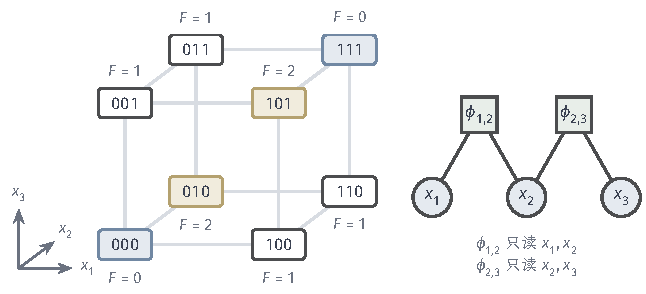
\includegraphics[width=109.269mm]{figures/01-basic-mathematics/04-graphs/tikz/c5-configuration-scopes/figure.pdf}
  \caption{配置空间与局部作用域。左：三个二值变量的$8$种配置排在立方体的顶点上，顶点旁的数是总成本$F=\phi_{1,2}+\phi_{2,3}$，其中相邻变量取值不同时成本为$1$；蓝色顶点成本为$0$，黄色顶点成本为$2$。右：圆点表示变量，方块表示局部函数，连线表示该函数读取的变量。每个局部函数只读取两个变量，但它们的和仍然对全部$8$种配置给出成本。}
  \label{fig:graph-dp-configuration-scopes}
\end{figure}

把这个例子一般化。设有一组局部项，用下标$a\in A$区分，每一项$\phi_a$只读取下标集合$S_a\subseteq V$中的变量，总成本为
\begin{equation}
F(\bm x)=\sum_{a\in A}\phi_a(\bm x_{S_a}),\qquad \bm x\in\mathcal X .
\label{eq:graph-dp-local-sum}
\end{equation}
这里的$\phi_a$称为\term{局部函数}（local function），也常称为\term{因子}（factor）；它读取的下标集合$S_a$称为$\phi_a$的\term{作用域}（scope）。

“局部”限定的是读取范围，不是精度：$\phi_a$精确地给出$\bm x_{S_a}$每种取值的成本，并不是对某个整体函数的近似。作用域也不限于两个变量，三元、四元的局部函数同样允许；一元项$\phi_i(x_i)$是作用域为$\{i\}$的特例，作用域为空集的项是一个常数。

局部函数的取值允许为$+\infty$，用来表示禁止的组合。例如设备$1,2$不能同时打开时，可以令$\phi_{1,2}(1,1)=+\infty$。本部分固定如下运算约定：$+\infty$加任何有限数或$+\infty$仍得$+\infty$；比较大小时$+\infty$大于每个实数，因而有限集合中只要有一个有限数，最小值就是有限的。这样，只要某一项禁止，整个配置的总成本就是$+\infty$。

总成本有限的配置称为\term{可行配置}。同一个式~\eqref{eq:graph-dp-local-sum}因此既表达偏好，也表达约束。若最小值为$+\infty$，说明每个配置都被某项禁止，所以求最小值同时回答了是否存在可行配置。

式~\eqref{eq:graph-dp-local-sum}的分解由问题给出，不是自动成立的性质。任意函数$F$都可以写成作用域为$V$的单个“局部”函数，但这时局部函数表就有$|\mathcal X|$项，与直接枚举没有区别。本部分始终假定分解已经给定，并且各作用域都较小；从一个任意给定的整体函数中寻找小作用域分解，是另一个问题。

\subsection{依赖图与因子图}
\label{sec:graph-dp-factor-graphs}

要利用“某一项不读某个变量”，首先要知道哪些变量出现在同一个局部函数里。这是一种纯粹的结构信息，可以用几种图来记录，它们保留和丢失的内容各不相同。

只有成对局部项时，可以以变量为顶点，两个变量出现在同一个成对项中就连一条边。三台设备的例子得到路径$1-2-3$。这样的图记录的是函数的依赖关系，不是变量的取值本身；称“依赖结构是一条链”或“是一棵树”，指的就是这个依赖图是路径或树。

三元及更高阶的局部项无法用一条边表示。这时把变量和局部函数分成两类节点：每个变量一个圆形节点，每个局部函数一个方形节点；变量属于某个局部函数的作用域时，在两者之间连边。这样得到的二部图称为\term{因子图}（factor graph）。因子图保留了每个局部函数的身份：两个不同的局部函数即使作用域相同，也是两个不同的方形节点。图~\ref{fig:graph-dp-configuration-scopes}右侧就是三台设备例子的因子图。

\paragraph{原始图与超图}
看一个含三元项的例子，后文称为\emph{三元作用域例子}：四个二值变量$x_1,\ldots,x_4$，两个局部函数$\phi_A(x_1,x_2,x_3)$与$\phi_B(x_2,x_3,x_4)$，作用域为$S_A=\{1,2,3\}$和$S_B=\{2,3,4\}$。它们的数值在下一小节给出，这里只看结构。

除因子图外，还有两种常用的结构表示。第一种不保留函数节点，把每个作用域内的变量两两连边，得到的图称为\term{原始关系图}（primal graph），简称原始图。这里原始图有边$\{1,2\},\allowbreak\{1,3\},\allowbreak\{2,3\},\allowbreak\{2,4\},\allowbreak\{3,4\}$，唯独缺少$\{1,4\}$，因为变量$1$和$4$从不出现在同一个局部函数中。每个作用域在原始图中都是两两相邻的顶点组。

第二种允许一条“边”包含任意多个顶点：每个作用域记为一条\term{超边}（hyperedge），由此得到\term{超图}（hypergraph）。这里超图有两条超边$\{1,2,3\}$和$\{2,3,4\}$。图~\ref{fig:graph-dp-three-representations}并排画出了三种表示。

\begin{figure}[!htb]
  \centering
  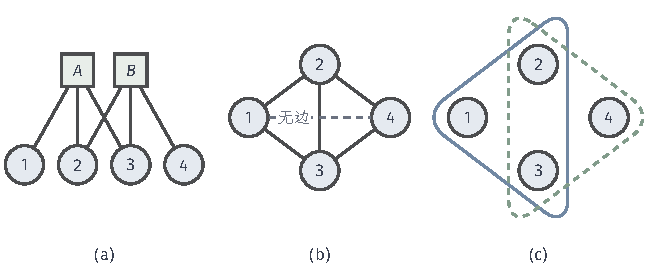
\includegraphics[width=111.936mm]{figures/01-basic-mathematics/04-graphs/tikz/c5-three-representations/figure.pdf}
  \caption{作用域$\{1,2,3\}$与$\{2,3,4\}$的三种结构表示。左：因子图，方块$A$、$B$是两个局部函数，连线表示读取关系。中：原始关系图，把每个作用域内的变量两两相连，只缺边$\{1,4\}$。右：超图，蓝色实线与绿色虚线围出的区域各是一条超边。若把两个三元函数换成五条边上的五个成对函数，原始图完全相同，而因子图和超图都会改变。}
  \label{fig:graph-dp-three-representations}
\end{figure}

\paragraph{原始图丢失的信息}
原始图丢失了作用域的分组：若把$\phi_A,\phi_B$换成定义在五条边上的五个成对局部函数，原始图不变，因子图和超图却不同。

更重要的是，相同的两两连接不能恢复函数表。设另有两个作用域同为$\{1,2,3\}$与$\{2,3,4\}$的局部函数：$\chi_A(x_1,x_2,x_3)$在$x_1+x_2+x_3$为偶数时取$0$、为奇数时取$+\infty$，$\chi_B$对$x_2+x_3+x_4$作同样的规定。$\chi_A$允许的取值恰为$(0,0,0),(0,1,1),(1,0,1),(1,1,0)$，其中任意两个变量的四种取值组合都出现过。

因此，若只保留“每对变量允许哪些取值”的成对规则，这些规则什么也不禁止，$16$种配置都会被放行。而原问题中$x_2,x_3$确定后，$x_1$和$x_4$都被奇偶条件唯一确定，只有$4$种可行配置。三元规则不是成对规则的叠加。

超图保住了作用域的分组，但和原始图一样不保存局部函数的数值；因子图保住了函数身份，也仍需另外存储每个函数的取值表。第~\ref{chap:general-graph-dp-construction}章构建计算结构时以原始图为依据，因为原始图上的边已经足以说明哪些变量必须同时出现，并且每个作用域都能整体放进构建出的某个计算单元（第~\ref{sec:graph-dp-clique-containment}小节）。计算时则始终使用完整的局部函数，不把它们拆成成对规则。

\subsection{计算任务与输出}
\label{sec:graph-dp-problem}

本部分的输入由两部分组成：每个变量的有限状态集合$\mathcal X_i$；一组局部函数$\phi_a$，每个以作用域$S_a$和一张取值表给出。取值表对$\bm x_{S_a}$的每种取值列出一个属于$\mathbb R\cup\{+\infty\}$的数，共$\prod_{i\in S_a}|\mathcal X_i|$项。在这同一份输入上，可以提出几种不同的计算任务。

最基本的任务是最小成本：
\begin{enumerate}
  \item 求最小成本$F^\star=\min_{\bm x\in\mathcal X}F(\bm x)$；
  \item 若$F^\star<+\infty$，给出一个最优配置$\bm x^\star$，即满足$F(\bm x^\star)=F^\star$的配置；若$F^\star=+\infty$，报告不存在可行配置。
\end{enumerate}

有时不想把全部变量都优化掉，而要保留一组变量$R\subseteq V$，对它们的每种取值给出其余变量取最优时的成本，即一张以$\bm x_R$为索引的表
\[
F_R(\bm x_R)=\min_{\bm x_{V\setminus R}}F(\bm x_R,\bm x_{V\setminus R}).
\]
这张表回答“若把这几个变量固定成某组值，最好能做到多少”。它的输出本身有$\prod_{i\in R}|\mathcal X_i|$项，$R=\varnothing$时退化为单个数$F^\star$。

另外两种任务不再挑选一个配置，而是对全部配置汇总。第一种是计数：可行配置有多少个。第二种是加权求和：给每个局部函数一张非负权重表，把配置的权重定义为各局部权重之积，求全部配置的权重总和。这两种任务的组合方式（相乘）和汇总方式（求和）都与最小成本不同，第~\ref{sec:graph-dp-semiring}节统一展开。

\paragraph{三元作用域例子的数值}
三元作用域例子的总成本为$F=\phi_A+\phi_B$，两张表由表~\ref{tab:graph-dp-ternary-tables}给出，其中$+\infty$表示禁止的组合。

\begin{table}[!htb]
  \centering
  \begin{tabular}{ccccccccc}
    \toprule
    取值 & $000$ & $001$ & $010$ & $011$ & $100$ & $101$ & $110$ & $111$\\
    \midrule
    $\phi_A(x_1,x_2,x_3)$ & $1$ & $0$ & $2$ & $+\infty$ & $0$ & $2$ & $1$ & $2$\\
    $\phi_B(x_2,x_3,x_4)$ & $2$ & $1$ & $0$ & $+\infty$ & $+\infty$ & $0$ & $1$ & $2$\\
    \bottomrule
  \end{tabular}
  \caption{三元作用域例子的两个局部函数。第一列的三位二进制串对$\phi_A$表示$(x_1,x_2,x_3)$，对$\phi_B$表示$(x_2,x_3,x_4)$。}
  \label{tab:graph-dp-ternary-tables}
\end{table}

最直接的做法是按字典序逐个检查全部配置，保留目前最小的成本$\hat F$（初始为$+\infty$）及其配置，遇到更小的成本就替换，全部检查完后停止。在这个例子上，枚举$16$个配置得$F^\star=0$，唯一的最优配置为$\bm x^\star=(0,0,1,0)$，可行配置共$10$个；后面用这一例子演示消元时，都用这一结果核对。

枚举总是正确，但要读$|\mathcal X|\cdot|A|$次表，各变量至多$q$个状态时可达$|A|\,q^n$。它把每个配置当作整体，没有利用“某一项不读某个变量”这一信息。下一节从链和树开始利用这一信息。

% 第11章第2节：链与树上的接口递推（固定接口后的子问题、链上的递推与回溯、树上的消息递推）。

\section{链与树上的接口递推}
\label{sec:graph-tree-dp}

依赖图没有环、局部项至多读取两个变量时，可以把变量分成只通过一个变量相连的两侧。本节先在小例子上看清“固定这个变量、分别处理两侧”为什么可行，以及要保留什么；再把这一动作在链上从一端推到另一端，在树上从叶推到根，每一步的接口都是单个变量。带环的情形留到下一节。

\subsection{固定接口后的子问题}
\label{sec:graph-dp-tree-idea}

\paragraph{接口变量}
回到第~\ref{sec:graph-dp-scopes}小节的三台设备。若先把$x_2$固定为某个值，$\phi_{1,2}$只剩$x_1$可变，$\phi_{2,3}$只剩$x_3$可变，两项不再共享任何变量，于是$x_1$和$x_3$可以分别选择：
\[
\min_{x_1,x_2,x_3}F=\min_{x_2}\Bigl[\min_{x_1}\phi_{1,2}(x_1,x_2)+\min_{x_3}\phi_{2,3}(x_2,x_3)\Bigr].
\]
对$x_2$的每个取值，两个内层最小值各只比较两个数。

这里$x_2$起着\term{接口}（interface）的作用：它把其余变量分成两侧，一侧的选择只通过$x_2$影响另一侧。好比两个房间之间只有一扇门，只要知道门开着还是关着，每个房间里怎样安排最好就可以各自决定。于是对接口的每种取值，先把一侧最好的成本算出来，记成一张以接口取值为索引的表，另一侧只需查表。

本部分反复使用的就是这个动作：固定一组接口变量，把只在一侧出现的变量汇总掉，留下一张以接口取值为索引的表。链和树上，接口可以沿依赖结构依次找到；一般依赖结构上接口要包含多个变量，怎样找到它们是第~\ref{chap:general-graph-dp-construction}章的问题。

\paragraph{成对成本的模型}
本节只考虑一元项和成对项，并假定成对项组成的依赖图没有环。这时总成本为
\begin{equation}
F(\bm x)=\sum_{i\in V}\phi_i(x_i)+\sum_{\{u,v\}\in E}\phi_{u,v}(x_u,x_v),
\label{eq:graph-dp-pairwise-cost}
\end{equation}
其中$\mathcal G=(V,E)$是依赖图，$\phi_{u,v}(x_u,x_v)$与$\phi_{v,u}(x_v,x_u)$指同一个局部函数。没有一元项的变量可以取$\phi_i\equiv0$。输入是各变量的状态集合、一元项表和每条边上的成对项表；输出是最小成本$F^\star$和一个最优配置，$F^\star=+\infty$时报告不可行。

\paragraph{三变量链}
先看三个变量的链$1-2-3$，每个变量取三档$\{0,1,2\}$，总成本$F=\phi_{1,2}(x_1,x_2)+\phi_{2,3}(x_2,x_3)$。两张局部函数表按行列给出：
\[
\bigl[\phi_{1,2}(x_1,x_2)\bigr]=\begin{bmatrix}4&1&3\\2&3&5\\3&4&2\end{bmatrix},\qquad
\bigl[\phi_{2,3}(x_2,x_3)\bigr]=\begin{bmatrix}1&3&2\\4&3&5\\2&2&4\end{bmatrix},
\]
左表的行对应$x_1=0,1,2$、列对应$x_2=0,1,2$，右表的行对应$x_2$、列对应$x_3$。直接枚举要计算$3^3=27$个配置的成本。

$x_1$只出现在$\phi_{1,2}$中。若先把$x_2$固定为某个值，$x_1$的选择就不再影响$\phi_{2,3}$，只需在左表的这一列中取最小。对$x_2=0,1,2$分别取列最小值，得到一张只依赖$x_2$的表
\[
m_{1\to2}(x_2)=\min_{x_1}\phi_{1,2}(x_1,x_2)=(2,\,1,\,2),
\]
达到最小值的$x_1$依次为$1,0,2$。这张表概括了链左端的全部信息：无论右侧怎样取值，只要$x_2$给定，左端最好的做法和它的成本都已确定。

剩下只需在$x_2,x_3$上求
\[
\min_{x_2,x_3}\bigl[m_{1\to2}(x_2)+\phi_{2,3}(x_2,x_3)\bigr].
\]
对$x_2=0,1,2$，括号内对$x_3$的最小值依次为
\[
2+1=3,\qquad 1+3=4,\qquad 2+2=4,
\]
所以最优成本为$3$，在$x_2=0,x_3=0$时达到，再查表得$x_1=1$。

整个过程计算了$9+9=18$个候选值，而不是$27$个配置；链越长，节省越多。

\paragraph{为什么要保留整张表}
左端交给右侧的必须是一张以接口取值为索引的表，而不只是左端的一个最优值。左表的最小值是$1$，在$(x_1,x_2)=(0,1)$处达到；若左端只报告“我最少付$1$，此时$x_2=1$”，右侧只能在$x_2=1$下选$x_3$，得到
\[
1+\min(4,3,5)=4.
\]
而整体最优配置$(1,0,0)$中左端付的是$\phi_{1,2}(1,0)=2$，比左端自己的最优值大，却让右端只付$1$。

左端事先无法知道右端偏好哪个$x_2$，所以要对接口的每个取值都给出条件最小成本，把选择$x_2$的决定留到两侧的成本都已知之后。

图~\ref{fig:graph-dp-interface-options}将左右两侧的条件最小值按$x_2$对齐。左侧最便宜的是中列，合并后最便宜的却是左列；保留整张表，才能把这一选择留给整体成本。

\begin{figure}[!htb]
  \centering
  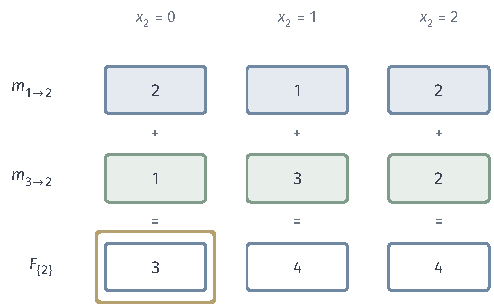
\includegraphics[width=83.608mm]{figures/03-graphs/04-local-functions-and-dynamic-programming/tikz/dp-interface-options/figure.pdf}
  \caption{接口表保留选择余地。沿用三档链的两张成本表，上排是对$x_1$取最小得到的$(2,1,2)$，中排是对$x_3$取最小得到的$(1,3,2)$，下排按同一$x_2$逐列相加。黄色边框标出整体最优值$3$所在的$x_2=0$，它并不对应上排的最小值。}
  \label{fig:graph-dp-interface-options}
\end{figure}

\paragraph{最小值的三条规则}
这样分步的依据是有限集合上最小值的三条规则。设$y,z$分别在有限集合中取值，$h$、$g$取值于$\mathbb R\cup\{+\infty\}$，$c$与$y$无关，则
\begin{equation}
\min_{y,z}h(y,z)=\min_{z}\min_{y}h(y,z),\qquad
\min_{y}\bigl[g(y)+c\bigr]=\min_{y}g(y)+c,
\label{eq:graph-dp-min-rules}
\end{equation}
并且对取值于互不相交变量组$y_1,\ldots,y_k$的函数，
\[
\min_{y_1,\ldots,y_k}\sum_{r}g_r(y_r)=\sum_r\min_{y_r}g_r(y_r).
\]

第一条成立，因为两边都是同一个有限数集中的最小元。第二条成立，因为加上同一个$c$不改变比较结果。第三条成立，因为各$y_r$可以分别取到各自的最小点，而任何选择都不会使某一项小于它的最小值。$c$或某项为$+\infty$时，按第~\ref{sec:graph-dp-scopes}小节的运算约定，三条规则依然成立。

在三变量链上，$\phi_{2,3}$对$x_1$而言是固定加项，由第一、二条，$\min_{x_1}$可以移到$\phi_{1,2}$上。

\subsection{链上的递推与回溯}
\label{sec:graph-dp-chain}

\subsubsection{问题与思路}

现在设链为$1-2-\cdots-n$，总成本含一元项$\phi_k(x_k)$和相邻成对项$\phi_{k-1,k}(x_{k-1},x_k)$。三变量链上的汇总可以从左端开始一步一步向右推进，每一步把接口右移一个变量。

推进到第$k$个变量时，左边的$x_1,\ldots,x_{k-1}$已经汇总掉，留下一张以$x_k$为索引的表$D_k(x_k)$：$x_k$取某个状态时，前$k$个变量的局部项
\[
\sum_{i=1}^{k}\phi_i(x_i)+\sum_{i=2}^{k}\phi_{i-1,i}(x_{i-1},x_i)
\]
对$x_1,\ldots,x_{k-1}$求最小值的结果，称为前$k$个变量的最小部分成本。这里$x_k$是已处理部分与其余部分之间的接口，$D_k$就是上一小节所说的条件最小成本表。

只有第一个变量时没有需要汇总的变量，$D_1(x_1)=\phi_1(x_1)$。从$D_{k-1}$得到$D_k$只需再汇总一个变量$x_{k-1}$：对$x_k$的每个状态，把前$k-1$个变量的最小部分成本加上连接两者的成对项，对$x_{k-1}$取最小值，再加上$x_k$自己的一元项，即
\begin{equation}
\begin{gathered}
D_1(x_1)=\phi_1(x_1),\\
D_k(x_k)=\phi_k(x_k)+\min_{x_{k-1}\in\mathcal X_{k-1}}\bigl[D_{k-1}(x_{k-1})+\phi_{k-1,k}(x_{k-1},x_k)\bigr],\quad k=2,\ldots,n.
\end{gathered}
\label{eq:graph-dp-chain-recursion}
\end{equation}
整条链的最小成本是
\[
F^\star=\min_{x_n}D_n(x_n).
\]
这种把问题按顺序拆开、为每个子问题保存最优值表并由前一张表算出后一张表的做法称为\term{动态规划}（dynamic programming）。

最小值只告诉我们最小成本是多少，不直接给出达到它的配置。取最小值时，“是哪一个$x_{k-1}$达到最小”被丢掉了；若只保存$D_k$，事后只能重新枚举。所以每算一个$D_k(x_k)$，都顺手记下达到最小值的$x_{k-1}$，组成\term{回溯表}$p_k(x_k)$。

算完以后从末端出发：$x_n$取使$D_n$最小的状态，再由$p_n(x_n)$读出$x_{k-1}$，逐个向左读到$x_1$。并列最优时需要事先固定选择规则，本节约定取编号最小的状态。

\subsubsection{算法实现}

链的次序、各变量的状态集合和局部函数表都由输入给定，运行中不变。算法维护三项状态：
\begin{itemize}
  \item 最小部分成本表$D_k$，$k=1,\ldots,n$：每张以$x_k$为索引，至多$q$项；初始只有$D_1=\phi_1$；
  \item 回溯表$p_k$，$k=2,\ldots,n$：$p_k(x_k)$是达到$D_k(x_k)$时$x_{k-1}$的取值；初始为空；
  \item 轮次$k$：已经算出的最后一张表的下标，初值为$1$。
\end{itemize}
此后每一轮令$k\gets k+1$，对$x_k$的每个状态$s$做两件事：
\begin{itemize}
  \item 列候选：对$x_{k-1}$的每个状态$r$，计算$D_{k-1}(r)+\phi_{k-1,k}(r,s)$，即式~\eqref{eq:graph-dp-chain-recursion}方括号中的值；
  \item 取最小：令$D_k(s)$等于一元项$\phi_k(s)$加上最小的候选值，$p_k(s)$为达到它的$r$，并列时取编号最小者。
\end{itemize}
第$n$轮之后递推停止。若$\min_{x_n}D_n(x_n)=+\infty$，报告不可行；否则按下面两步恢复配置：
\begin{itemize}
  \item 定末端：$x_n$取使$D_n$最小的状态，并列取编号最小者；
  \item 逆向读取：对$k=n,\ldots,2$，令$x_{k-1}=p_k(x_k)$。
\end{itemize}

\begin{algorithm}[链上的最小成本递推]
\label{alg:graph-dp-chain}
输入：链上各变量的有限状态集合、一元项表和相邻成对项表。输出：最小成本和一个最优配置。
\begin{enumerate}
  \item 令$D_1(x_1)=\phi_1(x_1)$。
  \item 对$k=2,\ldots,n$和每个$x_k$，计算式~\eqref{eq:graph-dp-chain-recursion}方括号中的全部候选值，取最小值记为$D_k(x_k)$，并把达到最小值的$x_{k-1}$（并列时取编号最小者）记为$p_k(x_k)$。
  \item 若$\min_{x_n}D_n(x_n)=+\infty$，报告不可行并停止。否则取使$D_n$最小的$x_n$（并列取编号最小者）；再对$k=n,\ldots,2$令$x_{k-1}=p_k(x_k)$。
\end{enumerate}
\end{algorithm}

\paragraph{执行过程}
取$n=4$的二值链，一元项为$\phi_1=(0,3)$、$\phi_2=(2,0)$、$\phi_3=(3,0)$、$\phi_4=(1,2)$，括号内依次是取$0$和取$1$的成本；相邻成对项在两端取值相同时为$0$，不同时为$2$。表~\ref{tab:graph-dp-chain-trace}列出各轮的候选与结果，逐轮看：
\begin{itemize}
  \item 第$1$轮：$D_1=\phi_1=(0,3)$。
  \item 第$2$轮：$x_2=0$的候选为$D_1(0)+0=0$与$D_1(1)+2=5$，加一元项$2$得$D_2(0)=2$；$x_2=1$的候选为$D_1(0)+2=2$与$D_1(1)+0=3$，加一元项$0$得$D_2(1)=2$。两处都由$x_1=0$达到，$p_2=(0,0)$。
  \item 第$3$轮：$x_3=0$的候选为$2,4$，加$3$得$5$；$x_3=1$的候选为$4,2$，加$0$得$2$。$D_3=(5,2)$，$p_3=(0,1)$。
  \item 第$4$轮：$x_4=0$的候选为$5,4$，加$1$得$5$；$x_4=1$的候选为$7,2$，加$2$得$4$。$D_4=(5,4)$，$p_4=(1,1)$。
\end{itemize}
第$4$轮后停止。$\min D_4=\min(5,4)=4$，在$x_4=1$处达到。沿回溯表逆向读取：
\[
x_3=p_4(1)=1,\qquad x_2=p_3(1)=1,\qquad x_1=p_2(1)=0,
\]
得到最优配置$(0,1,1,1)$。图~\ref{fig:graph-dp-chain-recursion}把同一过程画成每一轮的表和每个状态选中的前驱。

\begin{table}[!htb]
  \centering
  \small
  \begin{tabular}{@{}cccccccc@{}}
    \toprule
    & & \multicolumn{3}{c}{$x_k=0$} & \multicolumn{3}{c}{$x_k=1$}\\
    \cmidrule(lr){3-5}\cmidrule(lr){6-8}
    $k$ & $\phi_k$ & 候选 & $D_k(0)$ & $p_k(0)$ & 候选 & $D_k(1)$ & $p_k(1)$\\
    \midrule
    $1$ & $(0,3)$ & — & $0$ & — & — & $3$ & —\\
    $2$ & $(2,0)$ & $0,\ 5$ & $2$ & $0$ & $2,\ 3$ & $2$ & $0$\\
    $3$ & $(3,0)$ & $2,\ 4$ & $5$ & $0$ & $4,\ 2$ & $2$ & $1$\\
    $4$ & $(1,2)$ & $5,\ 4$ & $5$ & $1$ & $7,\ 2$ & $4$ & $1$\\
    \bottomrule
  \end{tabular}
  \caption{四变量二值链上的逐轮计算。“候选”一栏是式~\eqref{eq:graph-dp-chain-recursion}方括号中对$x_{k-1}=0,1$的两个值；$D_k$等于一元项加上候选中的较小者，$p_k$是达到较小者的$x_{k-1}$。}
  \label{tab:graph-dp-chain-trace}
\end{table}

\begin{figure}[!htb]
  \centering
  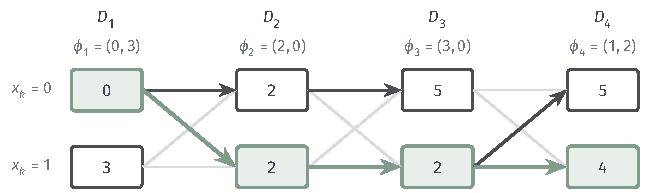
\includegraphics[width=109.587mm]{figures/01-basic-mathematics/04-graphs/tikz/c5-chain-recursion/figure.pdf}
  \caption{四变量二值链上的递推表。每列是一个变量，上下两格分别是$D_k(0)$与$D_k(1)$，列上方的小字为一元项。两列之间的灰色线表示全部候选，箭头从每个状态选中的前驱指向该状态，即回溯表$p_k$记录的选择。末列中$D_4(1)=4$最小，沿绿色箭头逆向读取得到最优配置$(0,1,1,1)$。逐点选取一元项最小的状态会得到$(0,1,1,0)$，成本为$5$。}
  \label{fig:graph-dp-chain-recursion}
\end{figure}

\subsubsection{算法分析}

\paragraph{正确性}
递推的正确性在于每张表$D_k$确实是前$k$个变量的最小部分成本。对$k$归纳。

$k=1$时没有被汇总的变量，结论就是定义。设结论对$k-1$成立。前$k$个变量的部分成本等于前$k-1$个变量的部分成本加上$\phi_{k-1,k}(x_{k-1},x_k)+\phi_k(x_k)$，后两项不含$x_1,\ldots,x_{k-2}$。按式~\eqref{eq:graph-dp-min-rules}的第一条，对$x_1,\ldots,x_{k-1}$求最小值可以先对$x_1,\ldots,x_{k-2}$、再对$x_{k-1}$进行；按第二条，先求的那一步可以越过后两项，只作用在前$k-1$个变量的部分成本上，由归纳假设得到$D_{k-1}(x_{k-1})$。

再对$x_{k-1}$求最小值，并把与$x_{k-1}$无关的$\phi_k(x_k)$移出，就得到式~\eqref{eq:graph-dp-chain-recursion}。取$k=n$，前$n$个变量的部分成本就是$F$，所以
\[
\min_{x_n}D_n(x_n)=F^\star.
\]

回溯得到的配置达到这个最小值。从末端起逐步向左，每一步选的$x_{k-1}=p_k(x_k)$都达到式~\eqref{eq:graph-dp-chain-recursion}中的最小值，于是读出的$x_1,\ldots,x_k$使前$k$个变量的部分成本恰好等于$D_k(x_k)$；读到$x_1$时，整个配置的成本等于$D_n(x_n)=F^\star$。这一论证要求$F^\star$有限；$F^\star=+\infty$时每个配置都“达到”最小值，所以算法报告不可行，而不输出配置。

\paragraph{与逐点选择的比较}
成对项正是逐点选择失效的原因。让每个变量只看自己的一元项、各自取最小，在上面的二值链中会选$(0,1,1,0)$：一元项合计为$1$，但两处取值变化要付$4$，总成本为$5$。递推得到的$(0,1,1,1)$在$x_4$上多付了$1$个单位的一元成本，却省掉了最后一处变化，总成本为$4$。$D_k$之所以能避免这种短视，是因为它对$x_k$的每个状态都保留了“左侧最好能做到多少”，等后面的变量看过成对项以后再决定$x_k$取哪个状态。

\paragraph{复杂度}
设每个变量至多有$q$个状态。每一轮为$x_k$的每个状态比较至多$q$个候选，共至多$q^2$次候选计算，整条链约$nq^2$次；$D_k$与$p_k$各至多$q$项，共约$2nq$项。若只要最优值而不恢复配置，任一时刻只需保留上一轮的表。与$q^n$个配置的枚举相比，开销从指数降为线性于$n$。

\subsection{树上的消息递推}
\label{sec:graph-dp-tree-messages}

\subsubsection{问题与思路}

树没有链那样的天然顺序，但选定一个根$\rho$以后，每个非根顶点都有唯一的父点（第~\ref{sec:graph-trees-forests}节）。链上的$D_{k-1}$概括了$x_k$左侧的全部变量；树上一个顶点可能有多个子点，每个子点下面挂着一棵子树，需要分别概括后再合并。

对树的一条边$\{u,v\}$，删去它以后树分成两部分，记含$u$的那部分顶点集为$V_{u|v}$，称为$u$一侧。$u$一侧的变量只通过这条边与其余部分发生联系，$x_v$就是这一侧与其余部分之间的接口：只要$x_v$给定，$u$一侧的变量最好怎样取值、最少要付多少成本就确定了。

把这个“最少要付多少”对$x_v$的每个状态列出来，就得到一张报价单：“你取$0$，我这边最少付多少；你取$1$，最少付多少”。$v$拿到报价单，不必知道$u$一侧有哪些变量、怎样取值，就能在决定自己的状态时把那一侧的成本算进去。

以图~\ref{fig:graph-dp-message-side}的五顶点树为例，删去边$\{3,4\}$后，$4$一侧是$\{4,5\}$。$x_3=0$时，这一侧最便宜的取法是$(x_4,x_5)=(0,1)$：一元项$\phi_4(0)+\phi_5(1)=0$，边$\{3,4\}$两端相同不付费，边$\{4,5\}$两端不同付$1$，合计$1$。

$x_3=1$时最便宜的是$(1,1)$，只付一元项$\phi_4(1)=1$。于是$4$向$3$报出的价目是$(1,1)$。

\begin{figure}[!htb]
  \centering
  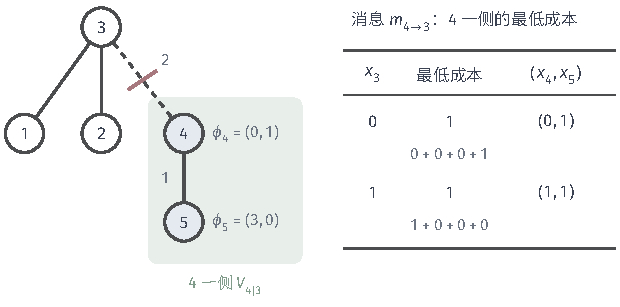
\includegraphics[width=104.902mm]{figures/01-basic-mathematics/04-graphs/tikz/c5-message-side/figure.pdf}
  \caption{消息是一侧的报价单。左：删去边$\{3,4\}$（虚线，旁边的$2$是两端取值不同时的成本），绿色区域是$4$一侧$V_{4|3}=\{4,5\}$，边$\{4,5\}$两端不同时成本为$1$。右：$x_3$取各状态时，$4$一侧的最低成本及达到它的取值；小字依次是$\phi_4$、$\phi_5$、边$\{3,4\}$、边$\{4,5\}$的成本。回溯表$b_{4\to3}$只记录其中$x_4$的取值$(0,1)$，$x_5$由$b_{5\to4}$给出。}
  \label{fig:graph-dp-message-side}
\end{figure}

这张报价单称为从$u$发往$v$的\term{消息}（message）。它可以逐层算出：$u$一侧除$u$本身以外，按$u$的其他邻居$r$分成几块，每块的最低成本已由消息$m_{r\to u}$报给$u$；$u$把自己的一元项、各块报来的价目和边$\{u,v\}$上的成对项相加，再替自己选最好的状态，即
\begin{equation}
\begin{aligned}
m_{u\to v}(x_v)=\min_{x_u\in\mathcal X_u}\Bigl[&\phi_u(x_u)+\phi_{u,v}(x_u,x_v)\\
&+\sum_{r\in N(u)\setminus\{v\}}m_{r\to u}(x_u)\Bigr],
\end{aligned}
\label{eq:graph-dp-tree-message}
\end{equation}
其中$N(u)$是$u$在依赖图中的邻居集合。消息等于$u$一侧在$x_v$固定时的最低成本，这一含义在第~\ref{sec:graph-dp-tree-analysis}小节证明。叶顶点只有一个邻居，求和为空，消息只由它自己的一元项和边上的成对项算出。链上的$D_k(x_k)$正是$\phi_k(x_k)+m_{k-1\to k}(x_k)$。

式~\eqref{eq:graph-dp-tree-message}右端用到$u$的其他邻居发来的消息，所以要从叶开始算，每个顶点等全部子点报完价再向父点报价；全部报到根以后，根把一元项与各条入消息相加，就得到整棵树在根取各状态时的最低成本。

与链上一样，取最小值丢掉了达到者，所以算每条消息时同时为接收端的每个状态$x_v$记下达到最小值的$x_u$，组成回溯表$b_{u\to v}(x_v)$。根选定状态以后，每个子点只需按父点的取值查自己的回溯表，就能沿树向外恢复整个配置。

\subsubsection{算法实现}

计算开始前任选根$\rho$，求出每个顶点的父点$p(u)$和一个后序，即先列出全部子点、再列出父点的顶点序列，可由一次深度优先遍历的完成次序得到。根、父点和后序只规定计算次序，运行中不变，与局部函数表一样不算状态。算法维护四项状态：
\begin{itemize}
  \item 消息表$m_{u\to p(u)}$，每个非根顶点$u$一张，以父点的取值$x_{p(u)}$为索引；初始均未计算；
  \item 回溯表$b_{u\to p(u)}$，与消息表一一对应，记录达到最小值的$x_u$；初始为空；
  \item 根处的合并值$g_\rho(x_\rho)$：根取各状态时整棵树的最低成本；向上一遍结束后才算出；
  \item 配置$\bm x$：初始各变量均未赋值，回溯时逐个写入。
\end{itemize}
向上一遍按后序依次处理非根顶点$u$，记$v=p(u)$。此时$u$的全部子点都已处理，消息$m_{r\to u}$都已算出。每处理一个顶点做三件事：
\begin{itemize}
  \item 汇总入消息：对$x_u$的每个状态，计算$\phi_u(x_u)+\sum_{r\in N(u)\setminus\{v\}}m_{r\to u}(x_u)$，即$u$及其子树在$x_u$固定时的最低成本；
  \item 列候选：对$x_v$的每个状态和$x_u$的每个状态，在上一步的值上加$\phi_{u,v}(x_u,x_v)$，得到式~\eqref{eq:graph-dp-tree-message}方括号中的值；
  \item 取最小：对$x_v$的每个状态，把最小的候选值记为$m_{u\to v}(x_v)$，达到它的$x_u$（并列取编号最小者）记为$b_{u\to v}(x_v)$。
\end{itemize}
全部非根顶点处理完后，在根处合并：
\[
g_\rho(x_\rho)=\phi_\rho(x_\rho)+\sum_{r\in N(\rho)}m_{r\to\rho}(x_\rho),
\]
最小成本为$\min_{x_\rho}g_\rho(x_\rho)$。若它为$+\infty$，报告不可行并停止；否则向外一遍恢复配置：
\begin{itemize}
  \item 定根：$x_\rho$取使$g_\rho$最小的状态，并列取编号最小者；
  \item 查表：按前序（后序的逆序，父点总在子点之前）处理非根顶点$u$，令$x_u=b_{u\to p(u)}(x_{p(u)})$。轮到$u$时父点已经赋值，所以查表总能进行。
\end{itemize}
每个非根顶点恰好赋值一次，全部变量赋值后停止。

\begin{algorithm}[树上的消息递推]
\label{alg:graph-dp-tree-messages}
输入：依赖树上各变量的有限状态集合、一元项表和各边的成对项表。输出：最小成本和一个最优配置，或不可行报告。
\begin{enumerate}
  \item 任选根$\rho$，求出父点$p(u)$与一个后序。
  \item 按后序处理每个非根顶点$u$，记$v=p(u)$：对$x_v$的每个状态，枚举$x_u$的全部状态，按式~\eqref{eq:graph-dp-tree-message}计算候选值，取最小者记为$m_{u\to v}(x_v)$，达到它的$x_u$（并列取编号最小者）记为$b_{u\to v}(x_v)$。
  \item 计算$g_\rho(x_\rho)=\phi_\rho(x_\rho)+\sum_{r\in N(\rho)}m_{r\to\rho}(x_\rho)$。若$\min_{x_\rho}g_\rho(x_\rho)=+\infty$，报告不可行并停止。
  \item 取使$g_\rho$最小的$x_\rho$（并列取编号最小者）；按前序对每个非根顶点$u$令$x_u=b_{u\to p(u)}(x_{p(u)})$。
\end{enumerate}
\end{algorithm}

\paragraph{执行过程}
沿用图~\ref{fig:graph-dp-message-side}的树：边为$\{1,3\},\allowbreak\{2,3\},\allowbreak\{3,4\},\allowbreak\{4,5\}$，以$3$为根；二值一元项为$\phi_1=(0,2)$、$\phi_2=(2,0)$、$\phi_3=(1,0)$、$\phi_4=(0,1)$、$\phi_5=(3,0)$；成对项在两端相同时为$0$，不同时分别为$1,1,2,1$（按上面边的顺序）。父点为$p(1)=p(2)=p(4)=3$、$p(5)=4$，取后序$1,2,5,4,3$。向上一遍依次处理四个非根顶点，表~\ref{tab:graph-dp-tree-trace}列出每条消息的候选：
\begin{itemize}
  \item 处理$1$：叶顶点，汇总值就是$\phi_1=(0,2)$。$x_3=0$的候选为$0+0$与$2+1$，$x_3=1$的候选为$0+1$与$2+0$，得$m_{1\to3}=(0,1)$，两处都由$x_1=0$达到，$b_{1\to3}=(0,0)$。
  \item 处理$2$：汇总值为$\phi_2=(2,0)$，得$m_{2\to3}=(1,0)$，$b_{2\to3}=(1,1)$：无论$x_3$取什么，$x_2$都取$1$更便宜。
  \item 处理$5$：汇总值为$\phi_5=(3,0)$，得$m_{5\to4}=(1,0)$，$b_{5\to4}=(1,1)$。
  \item 处理$4$：子点$5$的消息已经算出，汇总值为$\phi_4+m_{5\to4}=(0+1,\ 1+0)=(1,1)$。$x_3=0$的候选为$1+0$与$1+2$，$x_3=1$的候选为$1+2$与$1+0$，得$m_{4\to3}=(1,1)$，$b_{4\to3}=(0,1)$，与图~\ref{fig:graph-dp-message-side}右侧的报价一致。
  \item 根处合并：$g_3(0)=1+0+1+1=3$，$g_3(1)=0+1+0+1=2$。最小成本为$2$。
\end{itemize}
向外一遍从根开始，查表~\ref{tab:graph-dp-tree-trace}中接收端取$1$的回溯列：
\begin{itemize}
  \item 定根：$g_3=(3,2)$，取$x_3=1$；
  \item 按前序$3,4,5,2,1$查表：
  \[
  \begin{gathered}
  x_4=b_{4\to3}(1)=1,\qquad x_5=b_{5\to4}(1)=1,\\
  x_2=b_{2\to3}(1)=1,\qquad x_1=b_{1\to3}(1)=0.
  \end{gathered}
  \]
\end{itemize}
恢复的配置为$(x_1,\ldots,x_5)=(0,1,1,1,1)$。整个计算只算了$4$条消息，每条比较$4$个候选，而枚举需要$2^5=32$个配置。图~\ref{fig:graph-dp-tree-messages}画出了两遍的方向与次序。

\begin{table}[!htb]
  \centering
  \small
  \begin{tabular}{@{}ccccccc@{}}
    \toprule
    & \multicolumn{3}{c}{接收端取$0$} & \multicolumn{3}{c}{接收端取$1$}\\
    \cmidrule(lr){2-4}\cmidrule(lr){5-7}
    消息 & 候选 & 值 & 回溯 & 候选 & 值 & 回溯\\
    \midrule
    $m_{1\to3}$ & $0+0,\ 2+1$ & $0$ & $0$ & $0+1,\ 2+0$ & $1$ & $0$\\
    $m_{2\to3}$ & $2+0,\ 0+1$ & $1$ & $1$ & $2+1,\ 0+0$ & $0$ & $1$\\
    $m_{5\to4}$ & $3+0,\ 0+1$ & $1$ & $1$ & $3+1,\ 0+0$ & $0$ & $1$\\
    $m_{4\to3}$ & $0+0+1,\ 1+2+0$ & $1$ & $0$ & $0+2+1,\ 1+0+0$ & $1$ & $1$\\
    \bottomrule
  \end{tabular}
  \caption{分叉树上按后序计算的消息。“候选”一栏是式~\eqref{eq:graph-dp-tree-message}方括号中对$x_u=0,1$的两个值，每个值依次由一元项、边上成对项和子点消息相加；消息值取较小者，回溯表记录达到较小者的$x_u$。}
  \label{tab:graph-dp-tree-trace}
\end{table}

\begin{figure}[!htb]
  \centering
  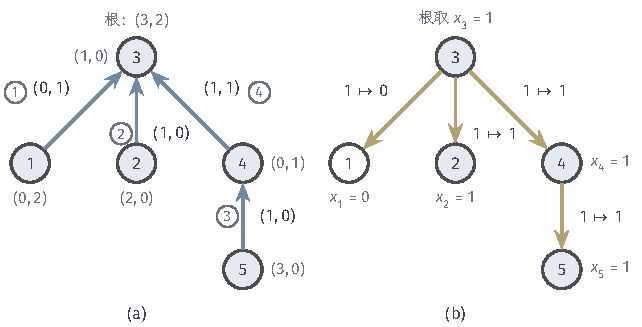
\includegraphics[width=108.514mm]{figures/01-basic-mathematics/04-graphs/tikz/c5-tree-messages/figure.pdf}
  \caption{分叉树上的消息与回溯。左：以$3$为根，按后序$1,2,5,4$发送消息；顶点旁的灰色二元组是一元项，箭头旁的二元组是消息表在接收端取$0$、$1$时的值，小圆圈中的序号是发送顺序；根合并后得到$(3,2)$。右：根取$x_3=1$后沿树向外查回溯表，黄色箭头旁的“$1\mapsto0$”表示父点取$1$时子点的最优选择为$0$；蓝色顶点取$1$，白色顶点取$0$，恢复的配置$(0,1,1,1,1)$成本为$2$。}
  \label{fig:graph-dp-tree-messages}
\end{figure}

把恢复的配置代回全部原始局部项，可以不依赖消息计算而独立核对结果。一元项依次为$0,0,0,1,0$，合计$1$；成对项中只有边$\{1,3\}$两端不同，贡献$1$；总成本为$2$，与根处的值一致，而且每个局部项只计了一次。

\subsubsection{算法分析}
\label{sec:graph-dp-tree-analysis}

\paragraph{正确性}
树上递推的正确性归结为一件事：每条消息确实是发送侧在接收端取值固定时的最低成本，即前面所说的报价单。

\begin{theorem}[树上消息的含义]
\label{thm:graph-dp-tree-message}
设依赖图$\mathcal G=(V,E)$是有限树，总成本由式~\eqref{eq:graph-dp-pairwise-cost}给出。对任意边$\{u,v\}$，记$F_{u|v}$为$u$一侧的部分成本：$V_{u|v}$中各顶点的一元项、两端都在$V_{u|v}$中的成对项，再加上边$\{u,v\}$上的$\phi_{u,v}$。则对每个$x_v$，
\[
m_{u\to v}(x_v)=\min_{\bm x_{V_{u|v}}}F_{u|v}(\bm x_{V_{u|v}},x_v).
\]
进一步，对任意根$\rho$，
\[
\min_{\bm x}F(\bm x)=\min_{x_\rho}\Bigl[\phi_\rho(x_\rho)+\sum_{r\in N(\rho)}m_{r\to\rho}(x_\rho)\Bigr].
\]
\end{theorem}

\begin{proof}
对$|V_{u|v}|$归纳。删去$u$以后，$V_{u|v}\setminus\{u\}$按$u$的其他邻居$r\in N(u)\setminus\{v\}$分成互不相交的部分$V_{r|u}$。由树中路径的唯一性，不同部分之间没有边，否则会与$u$形成环。因此$F_{u|v}$可以拆成
\[
F_{u|v}=\phi_u(x_u)+\phi_{u,v}(x_u,x_v)+\sum_{r\in N(u)\setminus\{v\}}F_{r|u},
\]
其中每个$F_{r|u}$只依赖$x_u$与$\bm x_{V_{r|u}}$，并且每个局部项恰好出现在其中一处。

固定$x_u$后，各$\bm x_{V_{r|u}}$是互不相交的变量组，由式~\eqref{eq:graph-dp-min-rules}后的第三条规则，对它们求最小值得到$\sum_r\min F_{r|u}$；由归纳假设，这个和等于$\sum_r m_{r\to u}(x_u)$。最后对$x_u$求最小值，就得到式~\eqref{eq:graph-dp-tree-message}。

叶顶点是归纳的起点，此时求和为空，结论直接由定义得出。根处的等式用同样的拆分得到：$V\setminus\{\rho\}$按$\rho$的邻居分成互不相交的部分，每部分的最小成本是一条入消息。
\end{proof}

链是树的特例：以$n$为根时$D_k(x_k)=\phi_k(x_k)+m_{k-1\to k}(x_k)$，定理再次给出$D_k$的含义。

回溯得到的配置也确实达到最优值。对子树大小归纳可知：若$x_v$已经确定，按回溯表给$u$一侧赋值后，$u$一侧的部分成本$F_{u|v}$恰好等于$m_{u\to v}(x_v)$，因为每一步选的$x_u$都达到式~\eqref{eq:graph-dp-tree-message}中的最小值，而子树内部又由归纳假设达到各条入消息的值。在根处合并后，总成本就等于根处的最小合并值。

这一论证要求根处最小值有限；为$+\infty$时任何配置都“达到”它，所以算法在这种情况下报告不可行，而不把回溯结果当作最优解输出。

回溯表只恢复一个最优配置。若要列出全部并列最优的配置，需要在每个状态记录全部最优选择，而这类配置的数目本身可能随$n$指数增长。

\paragraph{复杂度}
设每个变量至多有$q$个状态。处理非根顶点$u$时，汇总入消息需要对$x_u$的至多$q$个状态各加$|N(u)|-1$项，列候选与取最小共需至多$q^2$次加法和比较；对全部顶点求和，利用树中$\sum_u|N(u)|=2(n-1)$，向上一遍共需
\[
O\Bigl(\sum_u|N(u)|\,q+nq^2\Bigr)=O(nq^2)
\]
次运算。根处合并需要$O(|N(\rho)|q)$次，回溯只查$n-1$次表。存储为$n-1$张消息表和同样多的回溯表，每张至多$q$项。与$q^n$个配置的枚举相比，开销从指数降为线性于$n$，代价是要为每条边保存一张表。

\paragraph{适用范围}
本节的递推依赖两个条件。一是依赖图无环：定理的证明用到“删去$u$后各部分之间没有边”。二是局部项至多读取两个变量，使接口总是单个变量。依赖图含环时，删去一条边不再把变量分成两侧，单个变量不足以充当接口；下一节在四环上具体看这一点。

\subsubsection{各顶点的最小成本表}
\label{sec:graph-dp-tree-two-pass}

有时需要的不只是一个最优配置，而是每个顶点$v$取各状态$s$时整体能达到的最小成本$\min_{\bm x:\,x_v=s}F(\bm x)$，例如要知道某个变量换一个状态会多付多少。对根而言，这正是合并值$g_\rho$；对其他顶点，向上一遍只收集了来自子树一侧的消息，还缺父点一侧的报价。

所以再按前序从根向叶发送一遍消息，同样使用式~\eqref{eq:graph-dp-tree-message}：父点$v$向子点$u$发出的$m_{v\to u}$，汇总的是$v$的一元项、$v$的父点发来的消息和$v$的其他子点发来的消息。到达$u$时，$u$的全部邻居都已向它发过消息，把一元项与全部入消息相加，由定理~\ref{thm:graph-dp-tree-message}（以$u$为根）就得到$u$的最小成本表。两遍共发送$2(n-1)$条消息，开销仍为$O(nq^2)$。

图~\ref{fig:graph-tree-two-pass}只保留两遍发送的方向。第二遍仍然传递整张条件成本表；它与前面的回溯不同，回溯是在父点取值已经确定后读取一个达到者。

\begin{figure}[!htb]
  \centering
  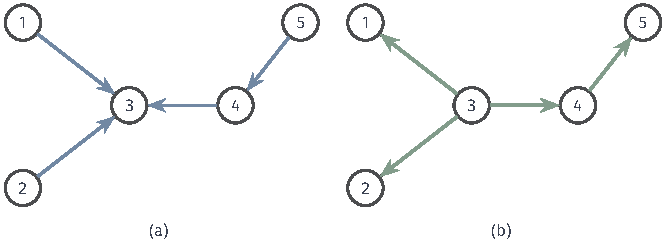
\includegraphics[width=107.500mm]{figures/03-graphs/04-local-functions-and-dynamic-programming/tikz/tree-two-pass/figure.pdf}
  \caption{两遍消息为每个顶点收齐各侧的信息。(a)以$3$为根，从叶向根传递蓝色消息；(b)按前序从根向外传递绿色消息，$3\to4$先于$4\to5$。两遍结束后每条无向边的两个方向都各发送一条表，共$2(n-1)$条；消息的索引是接收端的取值。}
  \label{fig:graph-tree-two-pass}
\end{figure}

在上例中，
\[
\begin{aligned}
m_{3\to1}(x_1)&=\min_{x_3}\bigl[\phi_3(x_3)+\phi_{1,3}(x_1,x_3)+m_{2\to3}(x_3)+m_{4\to3}(x_3)\bigr]\\
&=(2,1),
\end{aligned}
\]
其中$x_3=0,1$时一元项与两条入消息之和分别为$1+1+1=3$与$0+0+1=1$，再加上边$\{1,3\}$的成本取最小即得。于是$x_1$取$0$、$1$时的最小总成本为
\[
\phi_1+m_{3\to1}=(2,3).
\]

同样可得其余顶点的表：$x_2$为$(4,2)$，$x_3$为$(3,2)$，$x_4$为$(3,2)$，$x_5$为$(5,2)$。每张表的最小值都等于整体最优值$2$，并且都在最优配置$(0,1,1,1,1)$的相应分量处达到。

% 第11章第3节：从树到一般图（环带来的接口变化、四环算例、一般图动态规划的构建目标）。

\section{从树到一般图}
\label{sec:graph-dp-tree-to-general}

上一节的每一步都依赖一个事实：删去依赖树的一条边，变量就分成两侧，两侧只通过一个变量相连。依赖图含环时，这个事实不再成立。本节先说明环怎样改变接口，再用一个四环算例把变化落到具体数值上，最后说明一般图上的动态规划要事先构建什么。

\subsection{环带来的接口变化}
\label{sec:graph-dp-cycle-interface}

考虑四个变量排成的环$1-2-3-4-1$，每条边上有一个成对成本。删去边$\{1,2\}$后，剩下的是路径$2-3-4-1$，仍然连通：$x_1$不直接与$x_2$相连，却可以经由$x_4$和$x_3$影响$x_2$的最优选择。因此，沿一条边传递一张只以$x_2$为索引的报价单，无法概括$x_1$一侧，因为根本不存在只经过$x_2$与其余部分相连的“$x_1$一侧”。

链和树上的做法可以换一种说法，使它不依赖“一侧”。叶顶点$u$只出现在$\phi_u$和$\phi_{u,p(u)}$两项中；计算消息$m_{u\to p(u)}$，就是把这两项相加后对$x_u$取最小，然后用得到的表替换这两项。这个动作对任意局部函数集合都有意义。

设当前有一组函数，要汇总变量$x_i$。先找出当前全部作用域含$i$的函数，记为$\mathcal F_i$；它们的作用域之并去掉$i$，记为$S_i$。不含$i$的函数与$x_i$无关，可以留在最小化之外；含$i$的函数则必须一起处理。于是对$\bm x_{S_i}$的每种取值，把$\mathcal F_i$中的函数相加，再对$x_i$取最小，得到一个新函数
\begin{equation}
\psi_i(\bm x_{S_i})=\min_{x_i\in\mathcal X_i}\sum_{f\in\mathcal F_i}f .
\label{eq:graph-dp-elimination-step}
\end{equation}
然后从当前函数集合中删去$\mathcal F_i$，加入$\psi_i$；不含$i$的函数保持原样。这一操作称为消去$x_i$，按某个次序逐个消去变量的方法称为\term{变量消元}（variable elimination）。

消去$x_i$可以理解为替$x_i$提前做好决定。$x_i$的好坏只取决于$S_i$中那些与它同在某个函数里的变量；对这些变量的每一种取值，先算出$x_i$最好取什么、最少付多少，写成一张以$\bm x_{S_i}$为索引的表，此后其余变量只需查这张表，不必再关心$x_i$。由式~\eqref{eq:graph-dp-min-rules}的前两条，不含$i$的函数可以移出对$x_i$的最小化，所以替换前后，剩余变量每种取值下的最小成本不变；第~\ref{sec:graph-dp-min-cost-correctness}小节给出完整证明。

在树上消去叶顶点$u$时，$S_u=\{p(u)\}$，新函数就是消息$m_{u\to p(u)}$，接口仍是单个变量。在四环上消去$x_1$，情况不同：含$1$的函数是$\phi_{1,2}$与$\phi_{1,4}$，所以$S_1=\{2,4\}$，新函数$\psi_1(x_2,x_4)$同时读取$x_2$和$x_4$。在原来的环上，$2$与$4$并不相邻；消去$x_1$以后，它们通过$\psi_1$直接耦合在一起。

能否不要这张二元表，而给$2$和$4$各发一张单变量表？分别计算
\[
g(x_2)=\min_{x_1}\phi_{1,2}(x_1,x_2),\qquad h(x_4)=\min_{x_1}\phi_{1,4}(x_1,x_4)
\]
相当于允许两项各自为$x_1$挑选取值。由于每个$x_1$都满足$\phi_{1,2}+\phi_{1,4}\geq g(x_2)+h(x_4)$，对$x_1$取最小后总有
\[
g(x_2)+h(x_4)\leq\psi_1(x_2,x_4),
\]
但两边一般不相等：$x_1$只有一个，它在两项中必须取同一个值。下一小节的数值会说明，这个差异不仅是这一种拆法的缺陷，而且任何单变量表之和都无法代替$\psi_1$。

还有一种看似自然的做法，是在含环的依赖图上照搬式~\eqref{eq:graph-dp-tree-message}，让各顶点反复交换消息。这时同一部分成本会沿环被重复计入，上一节的正确性证明不再适用。这样的迭代是否收敛、收敛到什么，都需要另外分析；本部分只讨论精确计算。

\subsection{四环算例}
\label{sec:graph-dp-four-cycle}

本小节固定一个具体问题，后两章沿用它，分别演示两种结构构建和统一求值，避免更换例子掩盖它们之间的对应关系。四个二值变量$x_1,\ldots,x_4$排成环$1-2-3-4-1$，四条边上各有一个成对成本，没有一元项：
\begin{equation}
F(\bm x)=\phi_{1,2}(x_1,x_2)+\phi_{2,3}(x_2,x_3)+\phi_{3,4}(x_3,x_4)+\phi_{1,4}(x_1,x_4).
\label{eq:graph-dp-four-cycle}
\end{equation}
四张表由表~\ref{tab:graph-dp-four-cycle-costs}给出，每张表的行对应作用域中编号较小的变量。其中两个$+\infty$表示禁止的组合：$\phi_{3,4}(1,1)=+\infty$禁止$x_3,x_4$同时取$1$，$\phi_{1,4}(0,1)=+\infty$禁止$x_1=0$而$x_4=1$。

\begin{table}[!htb]
  \centering
  \begin{tabular}{cccc}
    \toprule
    $\phi_{1,2}(x_1,x_2)$ & $\phi_{2,3}(x_2,x_3)$ & $\phi_{3,4}(x_3,x_4)$ & $\phi_{1,4}(x_1,x_4)$\\
    \midrule
    $\begin{bmatrix}3&0\\1&2\end{bmatrix}$ &
    $\begin{bmatrix}1&3\\1&1\end{bmatrix}$ &
    $\begin{bmatrix}0&1\\0&+\infty\end{bmatrix}$ &
    $\begin{bmatrix}3&+\infty\\3&0\end{bmatrix}$\\
    \bottomrule
  \end{tabular}
  \caption{四环算例的局部成本。每张表的行对应作用域中编号较小的变量取$0,1$，列对应编号较大的变量取$0,1$；例如$\phi_{1,4}(0,1)=+\infty$。}
  \label{tab:graph-dp-four-cycle-costs}
\end{table}

\paragraph{枚举基准}
先用枚举给出核验基准。表~\ref{tab:graph-dp-four-cycle-enumeration}按字典序列出全部$16$个配置的总成本。其中$6$个配置被禁止：$x_4=1$而$x_1=0$的四个，以及$x_3=x_4=1$、$x_1=1$的两个。其余$10$个可行。

最小成本为$F^\star=3$，唯一的最优配置是$\bm x^\star=(1,0,0,1)$，此时四项依次为
\[
\phi_{1,2}(1,0)=1,\quad \phi_{2,3}(0,0)=1,\quad \phi_{3,4}(0,1)=1,\quad \phi_{1,4}(1,1)=0.
\]

\begin{table}[!htb]
  \centering
  \small
  \begin{tabular}{@{}cccccccc@{}}
    \toprule
    $0000$ & $0001$ & $0010$ & $0011$ & $0100$ & $0101$ & $0110$ & $0111$\\
    $7$ & $+\infty$ & $9$ & $+\infty$ & $4$ & $+\infty$ & $4$ & $+\infty$\\
    \midrule
    $1000$ & $1001$ & $1010$ & $1011$ & $1100$ & $1101$ & $1110$ & $1111$\\
    $5$ & $3$ & $7$ & $+\infty$ & $6$ & $4$ & $6$ & $+\infty$\\
    \bottomrule
  \end{tabular}
  \caption{四环算例全部配置的总成本。配置按$(x_1,x_2,x_3,x_4)$的字典序排列，前两行是$x_1=0$的八个配置，后两行是$x_1=1$的八个配置。}
  \label{tab:graph-dp-four-cycle-enumeration}
\end{table}

\paragraph{消去$x_1$}
按式~\eqref{eq:graph-dp-elimination-step}消去$x_1$。对$(x_2,x_4)$的每种取值，比较$x_1=0,1$两个候选$\phi_{1,2}(x_1,x_2)+\phi_{1,4}(x_1,x_4)$：
\[
\begin{aligned}
\psi_1(0,0)&=\min(3+3,\ 1+3)=4,&\qquad \psi_1(0,1)&=\min(3+\infty,\ 1+0)=1,\\
\psi_1(1,0)&=\min(0+3,\ 2+3)=3,&\qquad \psi_1(1,1)&=\min(0+\infty,\ 2+0)=2,
\end{aligned}
\]
达到最小值的$x_1$依次为$1,1,0,1$。

与之比较，分别取最小的单变量表是
\[
\begin{aligned}
g(x_2)&=\min_{x_1}\phi_{1,2}(x_1,x_2)=(1,0),\\
h(x_4)&=\min_{x_1}\phi_{1,4}(x_1,x_4)=(3,0).
\end{aligned}
\]
它们的和在$(x_2,x_4)=(1,1)$处为$0$，而$\psi_1(1,1)=2$：$g(1)=0$要求$x_1=0$，$h(1)=0$要求$x_1=1$，两项选的$x_1$互相矛盾。

更进一步，任何形如$g'(x_2)+h'(x_4)$的有限函数都满足
\[
\bigl[g'(0)+h'(0)\bigr]+\bigl[g'(1)+h'(1)\bigr]=\bigl[g'(0)+h'(1)\bigr]+\bigl[g'(1)+h'(0)\bigr],
\]
而$\psi_1$不满足这一等式：
\[
\psi_1(0,0)+\psi_1(1,1)=6\neq4=\psi_1(0,1)+\psi_1(1,0).
\]
所以$\psi_1$不能拆成两张单变量表之和，消去$x_1$以后的接口必须是$\{2,4\}$这两个变量的联合取值。

\paragraph{完成求值}
消去$x_1$后，剩下的函数是$\psi_1(x_2,x_4)$、$\phi_{2,3}(x_2,x_3)$与$\phi_{3,4}(x_3,x_4)$，只涉及$x_2,x_3,x_4$三个变量。把三项相加，按$(x_2,x_3,x_4)$的字典序得到
\[
(5,\ 3,\ 7,\ +\infty,\ 4,\ 4,\ 4,\ +\infty),
\]
最小值$3$在$(x_2,x_3,x_4)=(0,0,1)$处唯一达到。

再查$x_1$的选择：$(x_2,x_4)=(0,1)$时$x_1=1$。恢复的配置$(1,0,0,1)$与枚举结果一致。

这里同时处理的变量最多是三个：消去$x_1$时要看$\{1,2,4\}$的全部$8$种取值，最后又要看$\{2,3,4\}$的$8$种取值。第~\ref{chap:general-graph-dp-computation}章会把这一计算写成统一的递推，并用同一组数据检验最小成本、保留变量的成本表、计数和加权求和。

\subsection{一般图动态规划的构建目标}
\label{sec:graph-dp-construction-goal}

四环算例中的计算可以看成两个局部子问题。第一个子问题负责变量组$\{1,2,4\}$，固定接口$(x_2,x_4)$后汇总内部变量$x_1$，输出表$\psi_1$；第二个子问题负责$\{2,3,4\}$，读入$\psi_1$和其余两项，汇总全部剩余变量。链和树上的递推也是这样一族子问题，只是每个接口恰好是单个变量。

一般图上的动态规划要先构建这样一族子问题，它必须满足三项要求：
\begin{enumerate}
  \item 每个局部项都放进某个子问题，该子问题处理的变量包含它的整个作用域，并且每项只计一次；
  \item 摘要足够：一个子问题的内部变量与尚未处理部分的全部耦合都经过接口，所以以接口为索引的表不会丢失信息；
  \item 依赖可以排序：每个子问题只使用此前已完成的子问题的输出，最后汇总成整体结果。
\end{enumerate}
这三项都只涉及作用域和变量组，不涉及函数的具体数值，所以构建可以在求值之前单独完成。

树上递推正是满足这些要求的特例。把依赖树的一元项和成对项作为局部函数，按后序消去非根顶点：轮到$u$时，它的子点都已消去，子点留下的新函数与$\phi_u$、$\phi_{u,p(u)}$是仅有的含$u$的函数，所以$S_u=\{p(u)\}$，新函数$\psi_u$就是消息$m_{u\to p(u)}$，达到最小值的$x_u$就是回溯表$b_{u\to p(u)}$。

构建这族子问题有两种描述方式。变量消元用一个处理次序生成它们：每一步处理的变量组是当前变量及其$S_i$，新函数交给后面第一个用到它的步骤。树分解则把变量组（称为袋）和它们之间的接口显式组织成一棵树。第~\ref{chap:general-graph-dp-construction}章说明这两种构建怎样互相转换、怎样衡量其规模、怎样构造；第~\ref{chap:general-graph-dp-computation}章在构建好的结构上完成数值计算。四环算例已经显示，构建的质量体现为最多同时处理多少个变量，这里是三个。

\FloatBarrier
\section{本章小结}
\label{sec:tree-dp-chapter-summary}

本章的问题由局部函数组成：每个变量取有限个状态，整体成本是若干局部项之和，每一项只读取作用域中的少数变量，取值$+\infty$表示禁止的组合。同一份输入可以提出不同的输出要求：最小成本与一个最优配置、保留一组变量后的条件最小成本表、可行配置的个数，以及按局部权重之积定义的加权总和。枚举总能回答这些问题，但开销随变量数指数增长。

记录结构的几种图各有分工。原始图记录哪些变量共同出现，超图保留作用域的分组，因子图保留每个局部函数的身份；三者都不保存数值，原始图也不能恢复高阶规则，奇偶约束的例子说明三元规则不是成对规则的叠加。计算时始终使用完整的局部函数表。

链和树上之所以能精确递推，是因为删去依赖树的一条边就把变量分成两侧，两侧只通过一个接口变量相连。固定接口取值后，一侧的内部变量可以单独优化，结果写成以接口取值为索引的条件最小成本表；必须保留整张表，而不是一侧自己的最优值，因为接口最终取什么要等另一侧的成本也已知后才能决定。链上的递推、树上的消息和回溯表都是这一动作的具体形式，正确性来自有限集合上最小值的分步、移项和分离规则，开销对变量数是线性的。

依赖图含环时，单个变量不再能分隔两侧。消去一个变量会把它的邻居通过新函数耦合起来；四环算例中，消去$x_1$得到的$\psi_1(x_2,x_4)$不能拆成两张单变量表之和，接口必须同时保留两个变量。因此，一般图上的动态规划要先构建一族局部子问题，使每个局部项有处可放、接口足以概括内部变量、子问题的依赖可以排序；变量消元与树分解是描述这一构建的两种方式，分别在下一章建立并证明等价，数值计算统一放在第~\ref{chap:general-graph-dp-computation}章。


\chapter{一般图上动态规划的构建}
\label{chap:general-graph-dp-construction}

上一章的四环算例说明，依赖图含环时，消去一个变量会把它的邻居耦合起来，接口必须同时保留多个变量。于是在计算任何数值之前，要先回答：应当把哪些变量放在一起处理，每个子问题以哪些变量为接口，子问题之间按什么次序传递结果，才能保证每个局部项有处可放、每张摘要表不丢失信息？

本章只处理这个结构问题，输入是各局部函数的作用域，输出是一个可以核验的计算结构；具体数值表的计算留给下一章。第~\ref{sec:graph-dp-construction-problem}节写清输出要求，引入袋、接口和树分解，并说明保留变量的查询对结构提出什么额外要求。

随后两节从两个方向构建同一种结构。第~\ref{sec:graph-variable-elimination}节按一个消元次序模拟消元，用填充边记录新产生的耦合，把每一步同时处理的变量连成一棵树；第~\ref{sec:graph-dp-from-decomposition}节从一个给定的树分解出发，证明每个局部项都能放进某个袋、接口确实分隔两侧，并从叶袋读出一个相容的消元次序。

第~\ref{sec:graph-dp-construction-equivalence}节把两个方向合起来：消元得到的中间函数对应袋之间的接口消息，最小诱导宽度等于树宽，并在四环上把双向转换逐步做一遍。第~\ref{sec:graph-tree-decomposition-construction}节讨论怎样实际得到好的结构：贪心选择消元次序、利用弦图的完美消元序、借第~\ref{chap:minimum-spanning-tree}章的最大权生成树构造团树，以及怎样检验构建结果。

本章依赖上一章的消元操作式~\eqref{eq:graph-dp-elimination-step}与四环算例，以及第~\ref{sec:graph-trees-forests}节关于树的基本事实：树中两点之间的路径唯一，选根后每个非根节点有唯一的父节点。

% 第12章第1节：构建问题与输出要求（作用域与依赖图、袋与接口、树分解与树宽、接口与内部变量、保留变量的结构要求）。

\section{构建问题与输出要求}
\label{sec:graph-dp-construction-problem}

第~\ref{sec:graph-dp-construction-goal}小节提出了一般图上动态规划的三项要求：每个局部项有处可放，接口足以概括内部变量，子问题的依赖可以排序。本节把这些要求写成可以核验的定义。先固定构建的输入，再引入袋与接口，用树分解刻画合法的袋树，并说明每个子问题的接口与内部变量；最后说明保留变量的查询对结构提出什么额外要求。

\subsection{作用域与依赖图}
\label{sec:graph-dp-scope-graph}

构建的输入只是变量集合$V$和各局部函数的作用域$S_a$，$a\in A$，不含任何函数值。由它们得到第~\ref{sec:graph-dp-factor-graphs}小节的原始图$\mathcal G=(V,E)$：以全部变量为顶点，两个变量同属某个作用域时连一条边。每个作用域$S_a$在$\mathcal G$中两两相邻。

顶点集取全部变量，包括不出现在任何局部函数中的孤立变量。这样的变量不带来成本，但最优配置仍要给它赋值，计数时也要累计它的全部状态，所以它仍须出现在结构中。四环算例的作用域就是四条边，原始图就是环$1-2-3-4-1$本身；三元作用域例子的原始图有五条边，只缺$\{1,4\}$。

构建只使用作用域，所得结构对作用域相同而数值任意的全部问题都适用。某组特定数值可能恰好使一张中间表还能进一步分解（第~\ref{sec:graph-dp-fill-in}小节给出一例），但构建不利用这种巧合：一般数值下必须保留的耦合，构建时一律保留。数值上的进一步化简要回到函数表本身判断，不属于本章的结构问题。

\subsection{袋与接口}
\label{sec:graph-dp-bags}

回到四环算例。第~\ref{sec:graph-dp-four-cycle}小节的计算先同时看$\{1,2,4\}$，产生以$\{2,4\}$为索引的表$\psi_1$；再同时看$\{2,3,4\}$，读入$\psi_1$完成计算。三元作用域例子也一样：若按次序$(1,4,2,3)$消元，消去$x_1$时要同时处理$\{1\}\cup S_1=\{1,2,3\}$，消去$x_4$时处理$\{2,3,4\}$，随后依次处理$\{2,3\}$和$\{3\}$。

每一步产生的新函数会在后面某一步被用到：$\psi_1$与$\psi_4$都在消去$x_2$时被合并，消去$x_2$得到的新函数在消去$x_3$时被使用。

把每一步同时处理的变量集合看成一个节点，按“新函数交给哪一步使用”连接这些节点，就得到图~\ref{fig:graph-dp-bags-interface}中间的一棵树。这棵树只记录了哪些变量要一起处理、表交给谁，与$\phi_A,\phi_B$的具体数值无关，换一组作用域相同的函数，它照样适用。

准备放进同一张表里同时索引的变量集合称为\term{袋}（bag），可以把它想成计算时一次摆上桌面的变量：对它们的每一种联合取值各记一个数。袋组成的树称为袋树。袋树的节点是计算单元，袋树的边表示两个计算单元之间传递一张表；它与原始图中连接两个变量的边含义不同。不同的袋可以有公共变量，例如$\{1,2,3\}$与$\{2,3,4\}$都含$2,3$。

\begin{figure}[!htb]
  \centering
  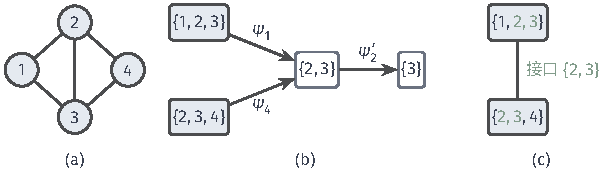
\includegraphics[width=103.283mm]{figures/01-basic-mathematics/04-graphs/tikz/c5-elimination-to-bags/figure.pdf}
  \caption{从消元步骤得到袋。左：三元作用域例子的原始图。中：按次序$(1,4,2,3)$消元时，每一步同时处理的变量集合构成一个袋，箭头表示新函数交给哪一步使用。右：$\{2,3\}$和$\{3\}$已包含在相邻的大袋中，并入后只剩两个袋，它们的交集$\{2,3\}$（绿色）就是接口。}
  \label{fig:graph-dp-bags-interface}
\end{figure}

袋与原始图中的团有关，但不必是团。原始图中两两相邻的顶点集合称为\term{团}（clique）。三元作用域例子中$\{1,2,3\}$是团，$\{1,2,4\}$不是，因为缺边$\{1,4\}$。四环算例中第一个袋$\{1,2,4\}$也不是原始图的团：$2$与$4$在环上不相邻，消去$x_1$后才通过$\psi_1$耦合。所以袋可以重叠，也可以含有原图中不相邻的变量。

\paragraph{接口与一致性}
在三元作用域例子中，袋$\{2,3\}$和$\{3\}$都已包含在相邻的大袋中，可以并入，最后只剩两个袋$\{1,2,3\}$与$\{2,3,4\}$，如图~\ref{fig:graph-dp-bags-interface}右侧。相邻两袋的交集称为它们的接口，这里是$\{2,3\}$；四环算例中两个袋的接口是$\{2,4\}$。这与第~\ref{sec:graph-dp-tree-idea}小节的接口变量含义相同，只是现在接口可以含多个变量。

接口上的变量在两个袋里是同一个变量，不是两个副本。左袋在汇总$x_1$时必须对$(x_2,x_3)$的每种取值分别给出结果，右袋使用这些结果时也必须按同样的$(x_2,x_3)$取值来读。左袋交出的正是一张以接口为索引的表。

两个袋之间只交换这样一张表，所以一个变量的取值也只能经接口从一个袋传到另一个袋，这就限制了袋的连接方式。若某个变量出现在两个不相邻的袋中，而连接它们的袋树路径上有某个袋不含这个变量，那么那个袋发出和收到的表都不以这个变量为索引，两侧便无法约定它取同一个值。另外，袋还必须能容纳所有局部函数，否则有的成本项无处计算。这两项要求合起来，就是下面的定义。

\subsection{树分解与树宽}
\label{sec:graph-tree-decomposition}
\label{sec:graph-dp-decomposition-definition}

在结构上，容纳局部函数的要求落实为每个变量和原始图的每条边都被某个袋包含；保持一致的要求就是上面的连接要求。

\begin{definition}[树分解]
\label{def:graph-dp-tree-decomposition}
设$\mathcal G=(V,E)$是有限无向图。$\mathcal G$的一个\term{树分解}（tree decomposition）由一棵有限树$\mathcal T$（节点集记为$T$）和每个节点$t\in T$上的子集$B_t\subseteq V$组成，满足：
\begin{enumerate}
  \item 顶点覆盖：每个顶点$v\in V$至少属于一个袋；
  \item 边覆盖：对每条边$\{u,v\}\in E$，存在某个袋同时含有$u$与$v$；
  \item 运行交集：对每个顶点$v\in V$，含$v$的节点集合$T_v=\{t\in T:v\in B_t\}$在$\mathcal T$中连通。
\end{enumerate}
第三个条件称为\term{运行交集性质}（running intersection property）。
\end{definition}

运行交集等价于：若$v$同时属于$B_s$和$B_t$，则$\mathcal T$中从$s$到$t$的路径上每个袋都含$v$。因为树中两点之间只有一条路径，$T_v$连通恰好意味着这条路径留在$T_v$中。直观地说，每个变量在袋树上占据一块连成一片的地盘；沿袋树行走，一个变量一旦离开就不会再出现。

\paragraph{梯子形图的分解}
图~\ref{fig:graph-dp-ladder-decomposition}中的梯子形图有两排顶点$1,2,3$与$4,5,6$，每排相邻顶点之间和同一列的两个顶点之间各有一条边。四个袋$\{1,2,4\},\allowbreak\{2,4,5\},\allowbreak\{2,3,5\},\allowbreak\{3,5,6\}$连成一条路径。

可以逐条核对定义。每个顶点都在某个袋中；七条边中，$\{1,2\},\{1,4\}$在第一个袋，$\{4,5\},\{2,5\}$在第二个袋，$\{2,3\}$在第三个袋，$\{5,6\},\{3,6\}$在第四个袋。

再看运行交集：含$2$的袋是前三个，含$5$的是后三个，含$4$的是前两个，含$3$的是后两个，都连成一段。

这个分解像一个窄窗口从左向右扫过梯子：每个袋是窗口某一时刻看到的顶点，相邻两袋的接口是窗口移动时必须记住的顶点。从第一个袋移到第二个袋时，$1$已经处理完毕，可以忘掉，只需记住$\{2,4\}$；之后$4$也处理完毕，只需记住$\{2,5\}$。运行交集保证被忘掉的顶点不会在后面的袋里再次出现，否则它的取值早已无从查找。梯子再长，窗口也只需同时看三个顶点；第~\ref{sec:graph-dp-chain}小节的链上递推是同样的扫描，只是每次只需记住一个变量。

\begin{figure}[!htb]
  \centering
  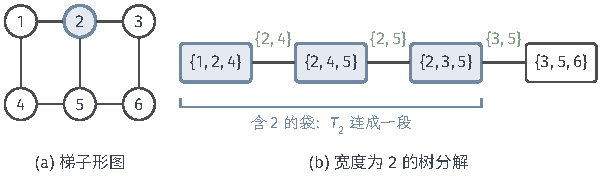
\includegraphics[width=101.85mm]{figures/01-basic-mathematics/04-graphs/tikz/c5-ladder-decomposition/figure.pdf}
  \caption{梯子形图的树分解。(a)两排顶点由三条横档相连。(b)四个袋连成一条路径，像窗口自左向右扫过梯子；边上的绿色集合是相邻两袋的接口，即窗口移动时要记住的顶点。蓝色的袋都含顶点$2$，它们连成一段，满足运行交集。}
  \label{fig:graph-dp-ladder-decomposition}
\end{figure}

\paragraph{运行交集的作用}
只覆盖顶点和边还不够。图~\ref{fig:graph-dp-running-intersection}比较路径$1-2-3-4$上的两种袋连接。两种连接使用同样的三个袋$\{1,2\},\allowbreak\{2,3\},\allowbreak\{3,4\}$，都覆盖了全部顶点和边。

上面一种按$\{1,2\}-\{2,3\}-\{3,4\}$连接，含$2$的两个袋相邻，含$3$的两个袋也相邻，是树分解。下面一种按$\{1,2\}-\{3,4\}-\{2,3\}$连接，含$2$的两个袋被不含$2$的袋$\{3,4\}$隔开。若沿这棵树计算，左端的袋可以选$x_2=0$，右端的袋可以选$x_2=1$，中间的袋不记录$x_2$，无从发现矛盾；拼起来的结果不对应任何一个配置。

\begin{figure}[!htb]
  \centering
  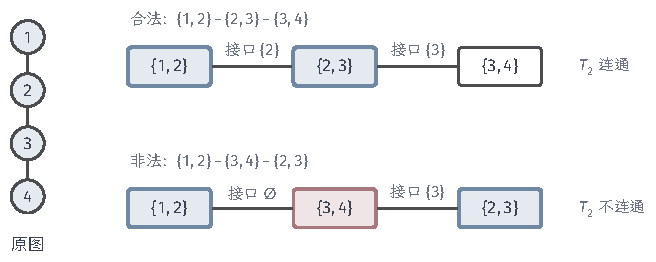
\includegraphics[width=111.016mm]{figures/01-basic-mathematics/04-graphs/tikz/c5-running-intersection/figure.pdf}
  \caption{路径$1-2-3-4$上的合法与非法袋连接。两种连接使用相同的三个袋，都覆盖全部顶点和边。上：含$2$的袋（蓝色）彼此相邻，含$3$的袋也相邻，满足运行交集。下：含$2$的两个袋之间隔着不含$2$的袋$\{3,4\}$（红色），$T_2$不连通，不是树分解。}
  \label{fig:graph-dp-running-intersection}
\end{figure}

\paragraph{宽度与树宽}
\label{sec:graph-dp-treewidth}
袋越大，袋表越大。为了用一个数概括一次分解的规模，定义树分解的宽度为
\[
\max_{t\in T}|B_t|-1,
\]
即最大袋的大小减一；图$\mathcal G$的\term{树宽}（treewidth）是它的全部树分解宽度的最小值，记为$\operatorname{tw}(\mathcal G)$。减一是一种约定，使得至少含一条边的树宽度恰为一。

把整个图放进一个袋总是合法的树分解，宽度为$|V|-1$，所以树宽总有定义，问题在于能否用更小的袋。直观地说，树宽回答的是：把这个图压成一棵树的形状时，每个树节点至少要装下多少个顶点。图越像树，需要的袋越小。

确定一个图的树宽需要两步：构造一个分解给出上界，再证明不存在更小宽度的分解给出下界。下面先给出几个小图的上界构造，图~\ref{fig:graph-dp-treewidth-examples}画出了相应的分解；下界的证明要用到第~\ref{sec:graph-dp-clique-containment}小节的团容纳引理，在那里补上。

单个顶点的图只需一个袋$\{1\}$，宽度为$0$，任何没有边的图都如此。至少含一条边的树有宽度为$1$的分解：任选根$\rho$，为每个非根顶点$u$建袋$\{u,p(u)\}$，其中$p(u)$是父点；若$p(u)$不是根，就把这个袋连到$p(u)$自己的袋上，根的各子点的袋则依次连成一条链。这样，非根顶点$v$出现在自己的袋和各子点的袋中，后者都与前者相邻；根只出现在各子点的袋中，它们连成链，所以运行交集成立。

四个顶点的环$1-2-3-4-1$有宽度为$2$的分解：两个袋$\{1,2,3\}$与$\{1,3,4\}$以一条边相连，接口为$\{1,3\}$；四环算例使用的$\{1,2,4\}$与$\{2,3,4\}$也是一个宽度为$2$的分解，接口为$\{2,4\}$。图~\ref{fig:graph-dp-ladder-decomposition}的梯子有宽度为$2$的分解。四个顶点两两相邻的完全图只用一个袋$\{1,2,3,4\}$，宽度为$3$。

\begin{figure}[!htb]
  \centering
  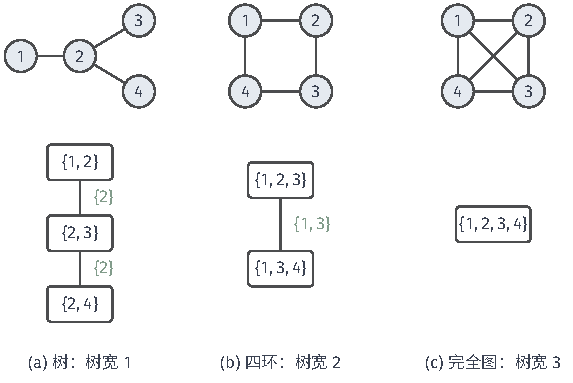
\includegraphics[width=96.95mm]{figures/01-basic-mathematics/04-graphs/tikz/c5-treewidth-examples/figure.pdf}
  \caption{三个四顶点图及其宽度最小的树分解，绿色集合是接口。(a)树：每条边一个袋，宽度为$1$。(b)四环：任何分解都有一个袋含三个顶点，宽度为$2$。(c)完全图：全部顶点必须同在一个袋中，宽度为$3$。}
  \label{fig:graph-dp-treewidth-examples}
\end{figure}

某一次构造得到宽度$k$，只说明$\operatorname{tw}(\mathcal G)\leq k$；要断言树宽恰为$k$，还需要证明不存在更小宽度的分解。

若每个变量至多有$q$个状态，宽度为$k$的分解中，每个袋至多有$k+1$个变量，稠密存储的袋表至多$q^{k+1}$项。这是第~\ref{chap:general-graph-dp-computation}章中主要的枚举规模。实际的总开销还包括袋的个数、接口的大小和每次读取局部函数的成本，宽度只控制其中随状态数指数增长的那一部分，第~\ref{sec:graph-dp-computation-cost}节再作完整分析。

寻找树宽最小的分解与使用一个已经给定的分解是两项不同的任务。前者在一般图上是困难的组合问题；后者只需按定义核验三个条件，再沿树计算。第~\ref{sec:graph-tree-decomposition-construction}节给出的构造方法都只保证得到合法的分解和宽度上界。

\subsection{接口与内部变量}
\label{sec:graph-dp-interface-internal}

一个树分解还要选定根，才能确定子问题的依赖次序。设已给袋树选根$r$，每个非根节点$u$有父节点$p(u)$。称
\[
S_u=B_u\cap B_{p(u)}
\]
为$u$的接口，$I_u=B_u\setminus S_u$为$u$的\term{内部变量}（internal variable）。根没有父节点，约定$S_r=\varnothing$、$I_r=B_r$。

节点$u$对应的子问题是：固定接口取值$\bm x_{S_u}$，汇总内部变量$\bm x_{I_u}$以及$u$下方各子问题已经汇总的内容，输出一张以$\bm x_{S_u}$为索引的表，交给父节点。接口为空时，这张表只有一项，是一个数。四环算例以$\{2,3,4\}$为根时，子节点$\{1,2,4\}$的接口为$\{2,4\}$，内部变量为$\{1\}$；根的内部变量为$\{2,3,4\}$。

为了让每个变量恰好被汇总一次，每个变量应当恰好是一个节点的内部变量。下面的引理说明运行交集保证了这一点，并指出是哪个节点。

\begin{lemma}[每个变量恰在一个袋中作内部变量]
\label{lem:graph-dp-unique-internal}
设$(\mathcal T,\{B_t\}_{t\in T})$是$\mathcal G$的树分解，袋树以$r$为根。对每个$v\in V$，$T_v$中有唯一一个离根最近的节点，记为$\operatorname{top}(v)$，$T_v$的每个节点都是它的后代（含它本身）；并且$v\in I_u$当且仅当$u=\operatorname{top}(v)$。
\end{lemma}

\begin{proof}
由顶点覆盖，$T_v$非空。取$T_v$中深度最小的一个节点$t$。若$y\in T_v$不是$t$的后代，从$y$到$t$的树上路径要先向上经过$y$与$t$的最近公共祖先$z$，而$z$比$t$更靠近根；由$T_v$连通，这条路径留在$T_v$中，于是$z\in T_v$，与$t$的选取矛盾。所以$T_v$的节点都是$t$的后代，深度最小的节点也只有$t$一个，记$\operatorname{top}(v)=t$。

若$u=\operatorname{top}(v)$是根，则$v\in B_r=I_r$。若它不是根，其父节点不是它的后代，因而不在$T_v$中，即$v\notin B_{p(u)}$，所以$v\in I_u$。反过来，若$u\in T_v$而$u\neq\operatorname{top}(v)$，则$u$是$\operatorname{top}(v)$的真后代，从$u$到$\operatorname{top}(v)$的路径第一步就到达$p(u)$；由运行交集，$p(u)\in T_v$，所以$v\in S_u$，不是$u$的内部变量。
\end{proof}

由此，构建的结果应当记录每个节点的袋$B_u$、父节点$p(u)$、接口$S_u$和内部变量$I_u$。这些都是结构信息；节点上要汇总哪些局部函数、汇总出的表取什么值，在第~\ref{chap:general-graph-dp-computation}章求值时确定。

\subsection{保留变量的结构要求}
\label{sec:graph-dp-query-structure}

第~\ref{sec:graph-dp-problem}小节的另一种输出是保留集$R\subseteq V$上的条件最小成本表$F_R(\bm x_R)$。这张表以$\bm x_R$的联合取值为索引，所以必须有某个计算单元同时看到$R$中的全部变量，并且在那之前不能把$R$中的任何变量汇总掉。

结构上采用两条要求。第一，在原始图中把$R$补成团，即在$R$的任意两个不相邻的变量之间加边，得到图$\mathcal G_R$，再为$\mathcal G_R$构建结构。第二，选取的根袋包含$R$。由第~\ref{sec:graph-dp-clique-containment}小节的团容纳引理，$\mathcal G_R$的任一树分解都有某个袋包含$R$，可以选它作根。

根袋包含$R$以后，$R$中每个变量$v$的$\operatorname{top}(v)$都是根，由引理~\ref{lem:graph-dp-unique-internal}，它们不会成为任何非根节点的内部变量，因而不会提前被汇总。根处只汇总$B_r\setminus R$，留下以$\bm x_R$为索引的表。用变量消元描述时，这相当于只消去$V\setminus R$中的变量，最后保留$R$（第~\ref{sec:graph-dp-order-to-decomposition}小节）。

补边可能增大宽度。路径$1-2-3$的树宽为$1$，若$R=\{1,3\}$，补边后得到三角形，树宽变为$2$。所以带保留变量的任务，其宽度要按$\mathcal G_R$计算，不能直接沿用不带查询时的最小树宽；输出表本身还有$\prod_{i\in R}|\mathcal X_i|$项。

在四环算例中取$R=\{1,3\}$。$1$与$3$在环上不相邻，补边$\{1,3\}$后，$\{1,2,3\},\{1,3,4\}$构成宽度为$2$的分解，两个袋都含$R$，任选一个作根即可。原来使用的分解$\{1,2,4\}-\{2,3,4\}$则没有袋同时含$1$和$3$，不能直接回答这个查询。

两个边界情形是：$R=\varnothing$时不加任何要求；$R=V$时$\mathcal G_R$是完全图，任何分解都有一个袋含全部变量，宽度为$n-1$，这与输出表本身就要列出全部配置一致。

% 第12章第2节：由变量消元构建动态规划（消元次序与填充图、消元簇与中间作用域、消元森林的构造、从消元簇得到树分解）。

\section{由变量消元构建动态规划}
\label{sec:graph-variable-elimination}

第~\ref{sec:graph-dp-cycle-interface}小节的消元操作每一步都产生一个新函数，它的作用域由当前所有含该变量的函数共同决定。本节说明，这些作用域可以只在原始图上模拟消元就预先算出，不需要任何函数值。按一个次序模拟一遍，就得到每一步同时处理的变量组和新函数交给哪一步使用，把它们连起来就是一个树分解。

\subsection{消元次序与填充图}
\label{sec:graph-dp-fill-in}

变量消元需要事先给定一个\term{消元次序}（elimination order）$\pi$，即全部要消去的变量的一个排列。消去一个变量时，新函数$\psi_i$的作用域$S_i$由所有含$i$的函数共同决定。在原始图上看，$S_i$恰好是$i$在当前原始图中的邻居集合，因为两个变量相邻当且仅当它们同在某个当前函数的作用域中。新函数读取这些邻居的联合取值，所以消元后的原始图中，这些邻居两两相邻。

\paragraph{一次消元的图操作}
在三元作用域例子中先消去$x_2$，就能看到这一点。$\phi_A$与$\phi_B$都含$2$，$S_2=\{1,3\}\cup\{3,4\}=\{1,3,4\}$，新函数
\[
\psi_2(x_1,x_3,x_4)=\min_{x_2}\bigl[\phi_A(x_1,x_2,x_3)+\phi_B(x_2,x_3,x_4)\bigr]
\]
同时读取$x_1,x_3,x_4$。按$(x_1,x_3,x_4)$的字典序，它的八个值为
\[
\psi_2=(3,\,2,\,0,\,+\infty,\,2,\,1,\,2,\,4),
\]
例如$(x_1,x_3,x_4)=(0,0,0)$处的两个候选为
\[
\phi_A(000)+\phi_B(000)=3,\qquad \phi_A(010)+\phi_B(100)=+\infty.
\]

原始图中原来没有边$\{1,4\}$，消元后必须补上，如图~\ref{fig:graph-dp-elimination-step}所示。这样为记录新函数的联合依赖而补入的边称为\term{填充边}（fill-in edge）。

填充边不表示原问题增加了约束，而是把原来经过$x_2$的间接联系直接记下来。看$x_3=1$的情形：$x_1=0$时，$\phi_A(0,1,1)=+\infty$迫使$x_2=0$，而$\phi_B(0,1,1)=+\infty$又禁止$x_4=1$；$x_1=1$时$x_2$可以取$1$，$x_4=1$仍然可行。原问题中$x_1$通过$x_2$牵制$x_4$。

消去$x_2$以后，这种牵制只能由$\psi_2$自己记录：上面的值中$\psi_2(0,1,1)=+\infty$，而$\psi_2(0,1,0)=0$、$\psi_2(1,1,1)=4$都有限。

若$\psi_2$能拆成一个$(x_1,x_3)$的函数与一个$(x_3,x_4)$的函数之和，固定$x_3=1$后就有
\[
\psi_2(x_1,1,x_4)=g(x_1)+h(x_4).
\]
由$g(0)+h(1)=+\infty$知$g(0)$或$h(1)$为$+\infty$，与$g(0)+h(0)$、$g(1)+h(1)$都有限矛盾。所以这张表必须同时以$x_1$和$x_4$为索引，填充边$\{1,4\}$反映的正是这一点。四环算例中消去$x_1$补入的边$\{2,4\}$也是如此（第~\ref{sec:graph-dp-four-cycle}小节）。

\begin{figure}[!htb]
  \centering
  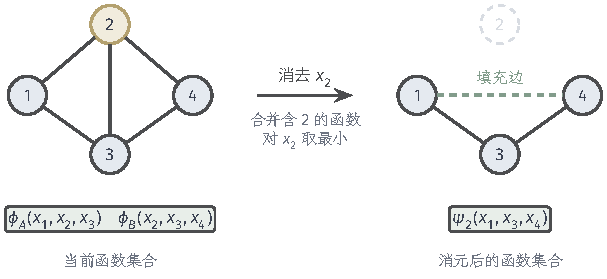
\includegraphics[width=102.687mm]{figures/01-basic-mathematics/04-graphs/tikz/c5-elimination-step/figure.pdf}
  \caption{消去$x_2$时的函数更新与图更新。左：消元前，黄色的$x_2$同时属于$\phi_A$与$\phi_B$的作用域，它的邻居是$1,3,4$。右：消元后，两个函数被新函数$\psi_2(x_1,x_3,x_4)$取代，$x_2$及其关联边被删除，邻居$1,3,4$两两相邻，其中绿色虚线$\{1,4\}$是填充边。}
  \label{fig:graph-dp-elimination-step}
\end{figure}

一般地，消元在原始图上对应一个纯粹的结构操作：把$i$的当前邻居两两连边，然后删去$i$及其关联边。不含$i$的函数提供的边保持不变；含$i$的函数在剩余变量之间提供的边都落在$S_i$内，已被补成的团覆盖；新函数$\psi_i$提供的边恰是$S_i$内的全部点对。因此，消元后函数集合的原始图恰好是对原始图执行这一操作的结果。对消元步数归纳，每一步的当前图都是当前函数集合的原始图，于是只看这个图操作，就能在不计算任何数值的情况下预先知道每一步的$S_i$。

\paragraph{填充图}
按次序$\pi$执行全部消元步骤，把途中补入的所有填充边加入原始图，得到的图称为$\pi$的\term{填充图}（filled graph），记为$\mathcal G^+_\pi$。它记录了这次消元中出现过的全部耦合：原始边来自局部函数，填充边来自中间函数。四环算例按次序$(1,2,3,4)$消元时只补入$\{2,4\}$，填充图是环加上弦$\{2,4\}$。第~\ref{sec:graph-dp-chordal}小节会说明填充图总是弦图。

\paragraph{作用域的结构上界}
图操作只预测新函数可能同时读取哪些变量，不计算新函数的取值，而对特殊的局部函数，新函数可能仍能进一步分解。例如，若$\phi_A(x_1,x_2,x_3)=g(x_1)+h(x_2,x_3)$，则
\[
\psi_2(x_1,x_3,x_4)=g(x_1)+\min_{x_2}\bigl[h(x_2,x_3)+\phi_B(x_2,x_3,x_4)\bigr],
\]
它是一个$x_1$的函数与一个$(x_3,x_4)$的函数之和，实际上并不需要同时索引$x_1$与$x_4$。但这时$\phi_A$本可以作为两个作用域更小的局部函数输入；只给作用域$\{1,2,3\}$时，填充边不知道这种数值巧合。所以补边图给出的是作用域给定、数值任意时新函数作用域的上界；第~\ref{sec:graph-dp-scope-graph}小节说过，构建只依据作用域，不利用这类数值上的巧合。

\subsection{消元簇与中间作用域}
\label{sec:graph-dp-elimination-clusters}

设消元次序为$\pi=(v_1,\ldots,v_n)$。消去$v_i$时，记它在当前图中的邻居集合为$S_i$，也记作$N^+_\pi(v_i)$；上标$+$表示这些邻居都排在$v_i$之后，因为排在前面的顶点已从当前图中删去。称
\[
B_i=\{v_i\}\cup S_i
\]
为第$i$步的\term{消元簇}（elimination cluster）；以顶点本身作下标时，也写作$B_{v_i}$、$S_{v_i}$。它是这一步同时处理的全部变量：计算新函数$\psi_i$要枚举$\bm x_{B_i}$的全部取值，而$\psi_i$的作用域是$S_i$。

消元簇有两条结构性质。第一，$B_i$在填充图中是团：$S_i$在第$i$步被补成团，$v_i$与$S_i$中每个顶点相邻。第二，原始图中排在$v_i$之后的邻居都在$S_i$中，因为在处理$v_i$之前只删去过已处理的顶点及其关联边。

消元次序$\pi$下的最大剩余邻居数$\max_i|S_i|$称为$\pi$的\term{诱导宽度}（induced width），它等于最大消元簇的大小减一。诱导宽度决定了这次消元中最多同时处理多少个变量。

在四环算例中按$(1,2,3,4)$消元：消去$1$时$S_1=\{2,4\}$，补入$\{2,4\}$，消元簇为$\{1,2,4\}$；消去$2$时当前邻居为$\{3,4\}$，其中$4$来自刚补入的填充边，消元簇为$\{2,3,4\}$；随后依次得到$\{3,4\}$和$\{4\}$。诱导宽度为$2$。

三元作用域例子按$(1,4,2,3)$消元，消元簇依次为
\[
 \{1,2,3\},\qquad \{2,3,4\},\qquad \{2,3\},\qquad \{3\},
\]
诱导宽度也是$2$。

\subsection{消元森林的构造}
\label{sec:graph-dp-order-to-decomposition}

\subsubsection{问题与思路}

输入是非空有限无向图$\mathcal G=(V,E)$（通常是局部函数的原始图）和一个消元次序；若有保留集$R$，图取补边后的$\mathcal G_R$，次序只排列$V\setminus R$。要求输出一个树分解，其袋是各步的消元簇，宽度等于诱导宽度。

第~\ref{sec:graph-dp-bags}小节已经从消元步骤读出过袋，这里把那个做法变成算法。消去$v_i$时同时处理的变量构成袋$B_i$。新函数$\psi_i$的作用域是$S_i$，它要等到$S_i$中第一个被消去的变量才会被用到，所以$B_i$应当连到那个变量的袋上。这正是图~\ref{fig:graph-dp-bags-interface}中按“新函数交给哪一步使用”连接袋的做法。

\paragraph{父袋容纳剩余作用域}
这种连接之所以合适，是因为父袋装得下整个$S_i$。设$v_j$是$S_i$中最早被消去的变量。第$i$步把$S_i$补成团；此后直到处理$v_j$之前，$S_i$中没有顶点被删去，因为它们都不早于$v_j$。所以处理$v_j$时，$S_i\setminus\{v_j\}$中的顶点都是$v_j$的当前邻居，即$S_i\setminus\{v_j\}\subseteq S_j$，从而
\[
S_i\subseteq B_j .
\]
也就是说，$\psi_i$交给的那一步恰好会枚举$\psi_i$所需的全部变量。

\paragraph{保留变量与分量}
有保留集$R$时，$R$中的变量不被消去，所有袋最后汇到一个根袋$B_R=R$。若$S_i$含待消去的变量，父袋仍取其中最早被消去者的袋，上面的论证不变，因为$R$中的变量从不删除。若$S_i$非空且全在$R$内，$\psi_i$只读取保留变量，就把$B_i$连到根袋$B_R$。

若$S_i=\varnothing$，$\psi_i$是一个常数，$B_i$没有父袋，成为一个分量的根。原图不连通时会出现多个这样的根；再用任意边把这些根（以及根袋$B_R$，若有）连成一棵树，这些边的接口为空，只用来把各分量的常数汇总起来。

\subsubsection{算法实现}

原图和次序在运行中不变；事先为每个顶点记下它在次序中的位置，以便比较先后。算法维护三项状态：
\begin{itemize}
  \item 当前图$\mathcal H$：用邻接集合存储，初值为$\mathcal G$（有保留集时为$\mathcal G_R$）的副本；
  \item 袋表：为每个已处理的顶点$v$记录袋$B_v$，初值为空；
  \item 父袋表：为每个袋记录它在袋树中的父袋，初值为空。
\end{itemize}
按次序逐个处理顶点，处理$v$时依次做四件事：
\begin{itemize}
  \item 读邻居：读出$v$在当前图$\mathcal H$中的邻居集合$N^+_\pi(v)$；
  \item 记袋：记录$B_v=\{v\}\cup N^+_\pi(v)$；
  \item 补团：把$N^+_\pi(v)$中尚不相邻的顶点两两连边，这些边就是填充边；
  \item 删点：从$\mathcal H$中删去$v$及其关联边。
\end{itemize}
这正是第~\ref{sec:graph-dp-fill-in}小节中消元在原始图上的结构操作。关键在于每一轮都要从更新后的图读取邻居，而不是从原图读取。全部待消去的顶点处理完后，再连接袋：
\begin{itemize}
  \item 对每个$N^+_\pi(v)$含待消去顶点的$v$，令$p(v)$为其中在次序里最早的顶点，把$B_{p(v)}$记为$B_v$的父袋；
  \item 对每个$N^+_\pi(v)$非空且包含于$R$的$v$，把根袋$B_R$记为父袋；
  \item $N^+_\pi(v)$为空的袋没有父袋，作为分量的根；若有多个根（连同$B_R$），用任意边把它们连成一棵树，这些边的接口为空。
\end{itemize}
不加空接口边时，这些袋和父袋连接按分量组成一片森林，称为$\pi$的\term{消元森林}（elimination forest）；加上空接口边后，它成为一棵袋树。

\begin{algorithm}[由消元次序构造树分解]
\label{alg:graph-dp-order-to-decomposition}
输入：非空有限无向图$\mathcal G$，可选的保留集$R$，以及$V\setminus R$的一个消元次序$\pi$。输出：$\mathcal G_R$的树分解，有保留集时根袋为$R$。
\begin{enumerate}
  \item 令$\mathcal H$为$\mathcal G_R$的副本（$R=\varnothing$时即$\mathcal G$），记下每个顶点在$\pi$中的位置。
  \item 按$\pi$依次取顶点$v$：读出$v$在$\mathcal H$中的邻居集合$N^+_\pi(v)$，记录$B_v=\{v\}\cup N^+_\pi(v)$；把$N^+_\pi(v)$中不相邻的顶点两两连边；从$\mathcal H$中删去$v$。
  \item 若$R\neq\varnothing$，建立根袋$B_R=R$。
  \item 对每个$v$：若$N^+_\pi(v)$含待消去的顶点，取其中位置最早的$p(v)$，连接$B_v$与$B_{p(v)}$；若$N^+_\pi(v)$非空且包含于$R$，连接$B_v$与$B_R$；若$N^+_\pi(v)=\varnothing$，$B_v$作为一个根。
  \item 若有多个根（连同$B_R$），用任意边把它们连成一棵树。
\end{enumerate}
\end{algorithm}

\paragraph{执行过程}
图~\ref{fig:graph-dp-elimination-to-decomposition}的例子有边$\{1,2\},\allowbreak\{1,4\},\allowbreak\{2,3\},\allowbreak\{3,4\},\allowbreak\{3,5\},\allowbreak\{4,5\}$，不保留变量，次序为$(1,2,5,3,4)$，表~\ref{tab:graph-dp-decomposition-trace}逐轮列出状态的变化。
\begin{itemize}
  \item 处理$1$：邻居为$\{2,4\}$，二者不相邻，补入填充边$\{2,4\}$，袋为$\{1,2,4\}$。
  \item 处理$2$：当前邻居$\{3,4\}$中的$4$来自上一轮补入的填充边，袋为$\{2,3,4\}$。若误从原图读取，袋就成了$\{2,3\}$，漏掉了消去$x_1$后新函数同时读取的$x_2,x_4$。
  \item 处理$5$：邻居$\{3,4\}$已经相邻，不补边，袋为$\{3,4,5\}$。
  \item 处理$3$与$4$：分别得到袋$\{3,4\}$与$\{4\}$，不再补边。
\end{itemize}
连接时，$B_1$的后续邻居中最早的是$2$，连到$B_2$；$B_2$与$B_5$的后续邻居都是$\{3,4\}$，连到$B_3$；$B_3$连到$B_4$；$B_4$没有后续邻居，作为根。得到以$B_4=\{4\}$为根的袋树，最大袋含$3$个顶点，宽度为$2$。

\begin{table}[!htb]
  \centering
  \caption{按次序$(1,2,5,3,4)$构造树分解时每一轮的状态。“当前邻居”从上一轮更新后的图读取；父袋在全部轮次结束后按“后续邻居中次序最早者”确定，最后一列是与父袋的接口。}
  \label{tab:graph-dp-decomposition-trace}
  \small
  \begin{tabular}{@{}ccccccc@{}}
    \toprule
    轮 & 处理 & 当前邻居 & 填充边 & 袋 & 父袋 & 接口\\
    \midrule
    $1$ & $1$ & $\{2,4\}$ & $\{2,4\}$ & $\{1,2,4\}$ & $B_2$ & $\{2,4\}$\\
    $2$ & $2$ & $\{3,4\}$ & 无 & $\{2,3,4\}$ & $B_3$ & $\{3,4\}$\\
    $3$ & $5$ & $\{3,4\}$ & 无 & $\{3,4,5\}$ & $B_3$ & $\{3,4\}$\\
    $4$ & $3$ & $\{4\}$ & 无 & $\{3,4\}$ & $B_4$ & $\{4\}$\\
    $5$ & $4$ & $\varnothing$ & 无 & $\{4\}$ & 根 & —\\
    \bottomrule
  \end{tabular}
\end{table}

\begin{figure}[!htb]
  \centering
  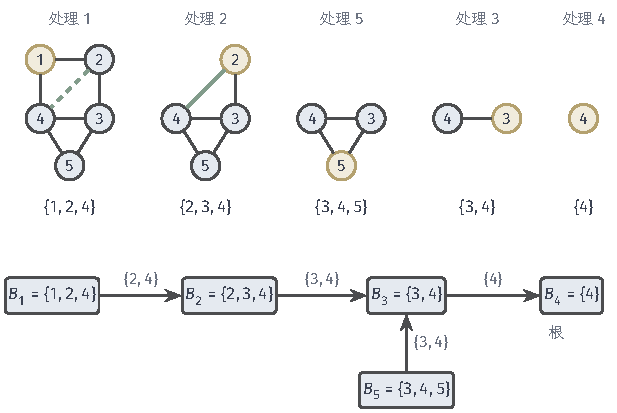
\includegraphics[width=104.369mm]{figures/01-basic-mathematics/04-graphs/tikz/c5-elimination-to-decomposition/figure.pdf}
  \caption{由消元次序$(1,2,5,3,4)$构造树分解。上行：每一轮的当前图，黄色为正在处理的顶点，绿色虚线为本轮补入的填充边，下一轮中它以绿色实线留在当前图里；图下标出记录的袋。下：按“连到最早被处理的后续邻居”连接父袋得到的袋树，箭头指向父袋，边旁标出接口。}
  \label{fig:graph-dp-elimination-to-decomposition}
\end{figure}

表中每个非根袋与父袋的接口恰好等于它的后续邻居集合。这不是巧合：父袋容纳$S_v$，而$v$本身比父袋的顶点都早被处理，不在父袋中，所以$B_v\cap B_{p(v)}=S_v$。第~\ref{sec:graph-dp-function-message-correspondence}小节会利用这一点把中间函数与袋之间的消息对应起来。

\subsection{从消元簇得到树分解}
\label{sec:graph-dp-clusters-to-decomposition}

下面的定理说明上述构造总是给出树分解，从而把消元过程中生成的依赖正式转成树分解，而不是另设一套独立的构建方法。

\begin{theorem}[消元次序产生树分解]
\label{thm:graph-dp-elimination-decomposition}
设$\mathcal G$是非空有限无向图，$R\subseteq V$，$\pi$是$V\setminus R$的消元次序。按算法~\ref{alg:graph-dp-order-to-decomposition}得到的袋树是$\mathcal G_R$的树分解，有保留集时根袋$B_R=R$；其宽度为$\pi$的诱导宽度与$|R|-1$中的较大者，无保留集时就是诱导宽度。特别地，$\mathcal G$的树宽不超过任何完整消元次序的诱导宽度。
\end{theorem}

\begin{proof}
先说明袋树是树。每个非根袋恰有一条通向父袋的边。父袋若为$B_{p(v)}$，则$p(v)$在次序中排在$v$之后，沿父边前进时次序位置严格增大；父袋若为$B_R$，则到达根袋。所以沿父边前进不会回到出发点，不形成环，每条父链都在有限步后到达一个根。各根之间再用树边连接，整体连通且无环。

顶点覆盖：待消去的$v$属于$B_v$，$R$中的顶点属于$B_R$。边覆盖：设$\{u,v\}$是$\mathcal G_R$的边。若两端都在$R$中，它被$B_R$覆盖。否则设$u$是两端中先被处理的待消去顶点；在处理$u$之前，图中只删去过已处理的顶点及其关联边，所以边$\{u,v\}$仍在，$v\in N^+_\pi(u)$，于是$B_u$同时含$u,v$。

运行交集：设$z\in B_v$且$z\neq v$，只需证明从$B_v$沿父链向上的每个袋都含$z$，直到到达$B_z$（$z$待消去时）或$B_R$（$z\in R$时）。这样含$z$的每个袋都与$B_z$或$B_R$由一条全部含$z$的路径相连，$T_z$连通。由$z\in N^+_\pi(v)=S_v$和上一小节的“父袋容纳剩余作用域”，父袋包含$S_v$，所以含$z$；若父袋是$B_{p(v)}$且$p(v)\neq z$，就对$p(v)$重复同样的论证。次序位置严格增大，最终到达$B_z$或$B_R$。

宽度：待消去顶点的袋大小为$|S_v|+1$，根袋大小为$|R|$，所以宽度如定理所述。最后，无保留集时树宽是全部树分解宽度的最小值，所以不超过诱导宽度。
\end{proof}

证明中的边覆盖论证同样适用于填充边，因此所得袋树也是填充图$\mathcal G^+_\pi$的树分解。

另一个直接推论是：每个局部函数的作用域$S_a$都整体落在某个袋中。取$S_a$中最先被处理的待消去变量$v$，$S_a$的其余变量在原始图中都与$v$相邻且排在$v$之后（或属于$R$），所以都在$S_v$中，$S_a\subseteq B_v$；若$S_a\subseteq R$，则$S_a\subseteq B_R$。第~\ref{sec:graph-dp-term-assignment}小节据此为局部项指定归属。

\paragraph{结构操作的代价}
设处理第$t$个顶点时它有$d_t$个当前邻居，补边要检查$\sum_t d_t(d_t-1)/2$对顶点，记录的袋共含$\sum_t(d_t+1)$个顶点。用支持常数时间查边和加边的邻接集合实现时，时间为
\[
O\Bigl(n+m+\sum_t d_t^2\Bigr),
\]
其中$m$是原始图的边数。这只是结构操作的开销；在袋上计算数值表时，开销随袋大小指数增长，第~\ref{sec:graph-dp-computation-cost}节另行计算。

% 第12章第3节：由树分解构建动态规划（包含局部作用域的袋、接口的分隔性质、从叶袋得到消元序）。

\section{由树分解构建动态规划}
\label{sec:graph-dp-from-decomposition}

上一节从消元次序出发得到树分解。本节反过来，从一个给定的树分解出发，直接规定局部子问题。需要证明的有两件事：每个局部项都能整体放进某个袋，这样它才有处可放；相邻两袋的接口确实把两侧的变量隔开，这样以接口为索引的摘要才足够。最后从叶袋向内处理变量，读出一个与分解相容的消元次序，说明树分解既能作为构建的输入，也能作为消元结果的显式表示。

\subsection{包含局部作用域的袋}
\label{sec:graph-dp-clique-containment}

计算时每个局部函数要整个放进一个袋，因为袋表需要同时索引它的全部变量。一个作用域$S_a$在原始图上是团：其中任意两个变量同在$\phi_a$中，因而相邻。但树分解的定义只要求每条边被某个袋覆盖，三个变量两两成边时，三条边似乎可能分别落在三个不同的袋中。下面先证明一个关于子树的一般事实，再由它推出这种情况不会发生。

把每个顶点$v$的出现位置$T_v$看成袋树中的一棵连通子树。若$u,v$相邻，边覆盖给出一个同时含$u,v$的袋，于是$T_u$与$T_v$相交。对一个团$C$，各$T_v$（$v\in C$）两两相交；要证明的是它们有一个公共节点。

\begin{lemma}[两两相交的子树有公共节点]
\label{lem:graph-dp-subtree-helly}
设$\mathcal T$是有限树，$T_1,\ldots,T_k$（$k\geq1$）是它的非空连通子树，并且两两相交。则存在节点同时属于全部$T_j$。
\end{lemma}

\begin{proof}
任取$\mathcal T$的一个节点作为根。与引理~\ref{lem:graph-dp-unique-internal}的证明相同，每个$T_j$有唯一一个离根最近的节点，记为$r_j$，并且$T_j$的每个节点都是$r_j$的后代（含$r_j$本身）。取$j^\ast$使$r_{j^\ast}$的深度在$r_1,\ldots,r_k$中最大，下面证明$r_{j^\ast}$属于每个$T_l$。

$l=j^\ast$时结论由定义成立。$l\neq j^\ast$时，$T_l\cap T_{j^\ast}$中有某个节点$x$；$x\in T_{j^\ast}$，因而$x$是$r_{j^\ast}$的后代。

考察$T_l$中从$x$到$r_l$的路径，它留在$T_l$中。若$r_l$不是$r_{j^\ast}$的后代，这条路径从$r_{j^\ast}$下方的子树走到外部，必须经过$r_{j^\ast}$，因为这棵子树与外部只通过$r_{j^\ast}$与其父节点之间的边相连；于是$r_{j^\ast}\in T_l$。若$r_l$是$r_{j^\ast}$的后代，则$r_l$的深度不小于$r_{j^\ast}$的深度；而按$j^\ast$的选取，$r_l$的深度又不大于$r_{j^\ast}$的深度，所以$r_l=r_{j^\ast}$，同样有$r_{j^\ast}\in T_l$。
\end{proof}

\begin{lemma}[团被某个袋容纳]
\label{lem:graph-dp-clique-in-bag}
设$(\mathcal T,\{B_t\}_{t\in T})$是$\mathcal G$的树分解，$C\subseteq V$是$\mathcal G$中的非空团，则存在节点$t\in T$使$C\subseteq B_t$。
\end{lemma}

\begin{proof}
由顶点覆盖与运行交集，每个$T_v$（$v\in C$）是非空连通子树。$C$中任意两个顶点$u,v$相邻，由边覆盖，$T_u\cap T_v\neq\varnothing$。由引理~\ref{lem:graph-dp-subtree-helly}，存在节点$t$属于全部$T_v$，即$C\subseteq B_t$。
\end{proof}

图~\ref{fig:graph-dp-clique-in-bag}画出了证明中的几棵子树：每个变量的出现位置向上延伸到自己的最高节点，最高节点最深的那个变量，它的最高节点被其余各子树“经过”，因而就是要找的袋。

\begin{figure}[!htb]
  \centering
  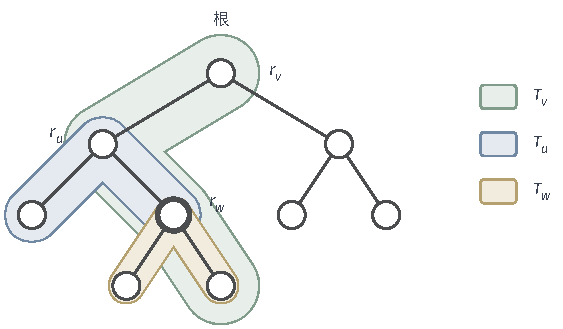
\includegraphics[width=102.648mm]{figures/01-basic-mathematics/04-graphs/tikz/c5-clique-in-bag/figure.pdf}
  \caption{团$\{u,v,w\}$被某个袋容纳的论证。袋树以顶部节点为根，三种颜色的区域分别是$T_u$、$T_v$、$T_w$，标签$r_u,r_v,r_w$标出各自离根最近的节点。$r_w$最深；$T_u$、$T_v$都要与$T_w$相交，而它们的最高节点不比$r_w$深，所以必须经过$r_w$。粗圈节点$r_w$的袋同时含$u,v,w$。}
  \label{fig:graph-dp-clique-in-bag}
\end{figure}

由引理~\ref{lem:graph-dp-clique-in-bag}，原始图的任一树分解中，每个局部函数的完整作用域都被某个袋整体容纳。因此在原始图上构造树分解就足够了，不需要额外记录高阶作用域；第~\ref{sec:graph-local-functions}节所说的“结构以原始图为依据、计算保留完整函数”在这里得到保证。

要找出容纳$S_a$的袋，只需在$T_v$（$v\in S_a$）中最小的一个里逐个检查袋是否包含$S_a$。同样，第~\ref{sec:graph-dp-query-structure}小节补成团的保留集$R$也一定被某个袋容纳。

\paragraph{树宽的下界}
引理~\ref{lem:graph-dp-subtree-helly}也给出第~\ref{sec:graph-tree-decomposition}小节几个例子的下界。一条边要求某个袋含两个顶点，所以含边的图宽度不能小于$1$；至少含一条边的树因而树宽恰为$1$。

四个顶点的环$1-2-3-4-1$没有宽度为$1$的树分解。给任一树分解选根，取环上的顶点$w$使$T_w$的最高节点最深。$w$在环上的两个邻居$u,v$各自与$w$相邻，于是$T_u$、$T_v$都与$T_w$相交；引理证明中的论证表明，$T_w$的最高节点同时属于$T_u$与$T_v$。这个袋含$u,v,w$三个顶点，所以宽度至少为$2$，四环的树宽恰为$2$。

这一论证对任何环都适用：含环的图树宽至少为$2$。因此树宽为$1$的图恰好是至少含一条边的森林。森林的各个分量分别按树的方法分解，再用任意的边把各分量的袋树连成一棵树；不同分量没有公共顶点，这些连接不影响运行交集。图~\ref{fig:graph-dp-ladder-decomposition}的梯子含环，又有宽度为$2$的分解，所以树宽恰为$2$；按同样的方式扫描，任意长的梯子树宽都是$2$。

四个顶点两两相邻的完全图恰好相反。整个顶点集是一个团，由引理~\ref{lem:graph-dp-clique-in-bag}，任何树分解都有一个袋装下全部四个顶点，宽度至少为$3$，所以树宽为$3$。同样，$n$个顶点的完全图树宽为$n-1$，树分解对它没有任何节省。

可见树宽衡量的是图与树的接近程度：一条边需要两个变量同时出现，一个环迫使某处至少三个变量同时出现，而一个大团迫使它的全部变量同时出现。

\subsection{接口的分隔性质}
\label{sec:graph-dp-interface-separation}

树上消息的正确性依赖于一件事：删去一条边后，两侧除了接收变量以外没有共同的变量。袋树上，这件事由运行交集保证。删去袋树边$\{s,t\}$后，袋树分成两部分；记$s$一侧全部袋中出现的变量为$V_{s|t}$，$t$一侧为$V_{t|s}$，接口为$B_s\cap B_t$。

若某个变量$v$在两侧都出现，从它在$s$侧的某个出现位置到$t$侧的某个出现位置，袋树路径必须经过边$\{s,t\}$；由运行交集，$B_s$与$B_t$都含$v$。所以
\begin{equation}
V_{s|t}\cap V_{t|s}\subseteq B_s\cap B_t,
\label{eq:graph-dp-interface-separation}
\end{equation}
即接口把两侧的变量隔开：固定接口取值后，两侧的其余变量互不重叠。

只有变量不重叠还不够，还要确认两侧没有被某个局部项直接连在一起，否则两侧的其余变量仍不能分别优化。下面的引理说明，每个局部项都整体落在某一侧。

\begin{lemma}[接口分隔两侧]
\label{lem:graph-dp-interface-separation}
设$(\mathcal T,\{B_t\}_{t\in T})$是原始图的树分解，$\{s,t\}$是袋树的边。则式~\eqref{eq:graph-dp-interface-separation}成立；并且对每个局部函数$\phi_a$，$S_a\subseteq V_{s|t}$或$S_a\subseteq V_{t|s}$。因此，任何局部项都不同时读取$V_{s|t}\setminus B_t$中的变量与$V_{t|s}\setminus B_s$中的变量。
\end{lemma}

\begin{proof}
式~\eqref{eq:graph-dp-interface-separation}已在上面证明。由引理~\ref{lem:graph-dp-clique-in-bag}，$S_a$被某个袋$B_x$容纳，$x$在$s$一侧或$t$一侧，于是$S_a\subseteq V_{s|t}$或$S_a\subseteq V_{t|s}$。若某个$\phi_a$同时读取$y\in V_{s|t}\setminus B_t$与$z\in V_{t|s}\setminus B_s$，不妨设$S_a\subseteq V_{s|t}$，则$z\in V_{s|t}\cap V_{t|s}\subseteq B_s$，与$z\notin B_s$矛盾；另一种情形同理。
\end{proof}

在选了根的袋树中，取$t=p(u)$。$u$下方各袋（含$u$本身）中出现而不在接口$S_u$中的变量，由式~\eqref{eq:graph-dp-interface-separation}不会出现在其余袋中，它们正是$u$下方各节点的内部变量之并。引理~\ref{lem:graph-dp-interface-separation}说明，固定$\bm x_{S_u}$后，这些变量与其余变量之间没有遗漏的直接耦合，所以$u$下方可以单独摘要成一张以$\bm x_{S_u}$为索引的表。这正是第~\ref{sec:graph-dp-construction-goal}小节的第二项要求；第~\ref{sec:graph-dp-min-cost-correctness}小节用它证明数值递推的正确性。

\subsection{从叶袋得到消元序}
\label{sec:graph-dp-decomposition-to-order}

给定一个宽度为$w$的树分解，可以反过来读出一个诱导宽度不超过$w$的消元次序。思路是从叶袋开始：叶袋中不在父袋里的变量只出现在这个叶袋中，消去它们时，它们的邻居都在叶袋里，产生的填充边也都落在叶袋里。

\paragraph{算法}
输入是图$\mathcal G$的一个树分解，选定一个根；输出是全部顶点的一个消元次序。维护当前图（初值为$\mathcal G$）、当前袋树（初值为输入分解）和已输出的次序（初值为空）。当前袋树不只一个节点时，反复处理一个非根叶节点$\ell$，记其父节点为$p$：
\begin{itemize}
  \item 若$B_\ell\subseteq B_p$，直接从袋树中删去$\ell$；
  \item 否则按任意次序依次消去$B_\ell\setminus B_p$中的变量：把每个变量追加到次序末尾，在当前图中把它的邻居补成团并删去它，同时把它从$B_\ell$中删去；此时$B_\ell\subseteq B_p$，再删去$\ell$。
\end{itemize}
最后只剩根袋，按任意次序消去其中剩余的变量。

\begin{algorithm}[由树分解读出消元次序]
\label{alg:graph-dp-decomposition-to-order}
输入：有限无向图$\mathcal G$的树分解，以及选定的根。输出：$\mathcal G$的一个消元次序。
\begin{enumerate}
  \item 令当前图为$\mathcal G$的副本，当前袋树为输入的分解，次序为空。
  \item 若当前袋树只剩根，转第4步。否则取一个非根叶节点$\ell$及其父节点$p$。
  \item 依次消去$B_\ell\setminus B_p$中的变量（追加到次序、补团、从当前图和$B_\ell$中删去），然后删去节点$\ell$，回到第2步。
  \item 按任意次序消去根袋中剩余的变量，输出次序。
\end{enumerate}
\end{algorithm}

\paragraph{正确性}
算法维持一个不变量：当前袋树（各袋只保留尚未消去的变量）是当前图的树分解。开始时它就是输入分解。

设叶节点$\ell$中有变量$v\notin B_p$。由运行交集，$T_v$连通，而$\ell$在袋树中只与$p$相邻、$p\notin T_v$，所以$T_v=\{\ell\}$：$v$只出现在$B_\ell$中。由边覆盖，$v$在当前图中的每条边都被某个含$v$的袋覆盖，只能是$B_\ell$，所以$v$的当前邻居全在$B_\ell$中，个数至多$|B_\ell|-1\leq w$。消去$v$补入的填充边两端都在$B_\ell$中，被$B_\ell$覆盖；从$B_\ell$中删去$v$后，三个条件对新的当前图仍然成立。

$B_\ell\subseteq B_p$时删去$\ell$也保持不变量：$\ell$覆盖的顶点和边都被$B_p$覆盖；含某个变量的节点集合去掉一个叶节点后仍然连通。最后剩下根袋时，当前图的全部顶点都在根袋中，每个顶点的当前邻居至多$|B_r|-1\leq w$个。

所以每个顶点被消去时，剩余邻居数都不超过$w$，得到的消元次序诱导宽度不超过分解的宽度。

\paragraph{执行过程}
以图~\ref{fig:graph-dp-ladder-decomposition}的梯子为例，以$\{3,5,6\}$为根，逐步处理叶袋：
\begin{itemize}
  \item 叶袋$\{1,2,4\}$的父袋是$\{2,4,5\}$，消去$1$：它的当前邻居为$\{2,4\}$，补入$\{2,4\}$；剩余的$\{2,4\}$包含于父袋，删去该叶。
  \item 接着$\{2,4,5\}$成为叶，消去$4$：当前邻居为$\{2,5\}$，已相邻。
  \item 再处理$\{2,3,5\}$，消去$2$：当前邻居为$\{3,5\}$，补入$\{3,5\}$。
  \item 最后在根袋中依次消去$3,5,6$。
\end{itemize}

得到的次序为$(1,4,2,3,5,6)$，各步剩余邻居数依次为$2,2,2,2,1,0$，诱导宽度为$2$，等于分解的宽度。每一步补入的填充边都落在当时的叶袋里，正如正确性论证所说。

% 第12章第4节：两种构建的等价关系（中间函数与接口消息的对应、树宽与最小诱导宽度、四环上的双向构建）。

\section{两种构建的等价关系}
\label{sec:graph-dp-construction-equivalence}

前两节分别从消元次序和树分解出发，构建出同一类结构。本节把两种表示逐项对照：消元簇对应袋，剩余作用域对应接口，中间函数对应向父袋传递的消息。比较规模时，要区分某一个构建的宽度与全部构建中的最优值；后者在两种表示下相等。最后在四环上把双向转换逐步做一遍。

\subsection{中间函数与接口消息的对应}
\label{sec:graph-dp-function-message-correspondence}

在算法~\ref{alg:graph-dp-order-to-decomposition}得到的袋树中，取消元森林的根为根。每个非根袋$B_i=\{v_i\}\cup S_i$与父袋的接口恰为$S_i$：第~\ref{sec:graph-dp-order-to-decomposition}小节已说明父袋包含$S_i$；另一方面，父袋若是$B_j=\{v_j\}\cup S_j$，其中的变量在处理$v_j$时都还在当前图中，而$v_i$此前已被删去，所以$v_i\notin B_j$，父袋若是根袋$B_R$，也因$v_i\notin R$而不含$v_i$。所以$B_i$的内部变量只有$v_i$一个，这与引理~\ref{lem:graph-dp-unique-internal}一致：$v_i$所在的最高节点就是$B_i$。

于是两种表示中的对象逐项对应：
\begin{itemize}
  \item 第$i$步的消元簇$B_i$对应袋树的一个节点；
  \item 中间函数$\psi_i$的作用域$S_i$对应该节点与父节点的接口；
  \item 消去$v_i$对应汇总该节点的内部变量；
  \item “$\psi_i$在消去$S_i$中最早的变量时被使用”对应“消息从子节点发往父节点”。
\end{itemize}
第~\ref{sec:graph-dp-elimination-message-correspondence}小节在相同的局部项归属下证明，按消元次序算出的$\psi_i$与沿袋树算出的消息逐项相等。

反过来，算法~\ref{alg:graph-dp-decomposition-to-order}从树分解读出消元次序时，处理叶袋$\ell$就是一次消息传递：消去$B_\ell\setminus B_p$中的变量，留下以$B_\ell\cap B_p$为作用域的结果交给父袋。一个袋可以有多个内部变量，相当于把连续的几步消元合并在一个计算单元里完成。

对应关系不要求逐表相同。把相邻的袋合并、把一个局部项从一个容纳它的袋移到另一个，都会改变中间表；只要结果仍是合法的树分解、每个局部项的作用域被所归的袋容纳、每项恰好归入一处，最终的最小成本、条件最小成本表、计数和加权总和都不变。这一点在第~\ref{chap:general-graph-dp-computation}章随各任务的正确性一起证明。

\paragraph{两种表示的组织差别}
两种做法的差别在于组织方式。变量消元边走边决定新函数交给谁，结构与数值交织在一起；树分解先把结构确定下来并核验，同一个分解可以用于作用域相同而数值不同的多组局部函数，也便于在不同的根下重复使用，例如第~\ref{sec:graph-dp-tree-two-pass}小节那样再发一遍反向消息，得到每个袋上的表。

\subsection{树宽与最小诱导宽度}
\label{sec:graph-dp-treewidth-induced-width}

定理~\ref{thm:graph-dp-elimination-decomposition}给出一个方向：每个消元次序都产生宽度等于其诱导宽度的树分解。第~\ref{sec:graph-dp-decomposition-to-order}小节给出另一个方向：每个宽度为$w$的树分解都读出诱导宽度不超过$w$的消元次序。两个方向合起来，得到下面的等式。

\begin{theorem}[树宽等于最小诱导宽度]
\label{thm:graph-dp-treewidth-induced-width}
设$\mathcal G$是非空有限无向图。则
\[
\operatorname{tw}(\mathcal G)=\min_{\pi}\ \max_{v}\ |N^+_\pi(v)|,
\]
其中$\pi$取遍全部顶点的消元次序，$N^+_\pi(v)$是按$\pi$消元时$v$的剩余邻居集合。
\end{theorem}

\begin{proof}
记右端为$w^\ast$，它是有限个次序上的最小值，因而可以达到。由定理~\ref{thm:graph-dp-elimination-decomposition}，诱导宽度为$w^\ast$的次序给出宽度为$w^\ast$的树分解，所以$\operatorname{tw}(\mathcal G)\leq w^\ast$。反过来，取宽度为$\operatorname{tw}(\mathcal G)$的树分解，由算法~\ref{alg:graph-dp-decomposition-to-order}及其正确性论证，得到诱导宽度不超过$\operatorname{tw}(\mathcal G)$的次序，所以$w^\ast\leq\operatorname{tw}(\mathcal G)$。
\end{proof}

这个等式说的是两种表示的最优值相等，不是两种对象一一对应。同一个树分解按不同的根、不同的叶袋处理次序可以读出许多消元次序；不同的消元次序也可能给出合并后相同的袋树。等式的用途是：寻找好的结构时，可以在消元次序上搜索，也可以在树分解上搜索，二者的最优规模相同。对某一个具体次序或分解，它的宽度只是树宽的上界。

\subsection{四环上的双向构建}
\label{sec:graph-dp-four-cycle-construction}

现在在四环算例上把两个方向逐步做一遍。原始图是环$1-2-3-4-1$。

\paragraph{由消元次序到袋树}
按次序$(1,2,3,4)$执行算法~\ref{alg:graph-dp-order-to-decomposition}，表~\ref{tab:graph-dp-four-cycle-construction}列出每一轮的状态。消去$1$时补入填充边$\{2,4\}$；消去$2$时当前邻居为$\{3,4\}$，已经相邻；之后不再补边。

\begin{table}[!htb]
  \centering
  \caption{四环上按次序$(1,2,3,4)$构建袋树。“当前邻居”从上一轮更新后的图读取；父袋按“后续邻居中次序最早者”确定，最后一列是与父袋的接口，它恰好等于当前邻居集合。}
  \label{tab:graph-dp-four-cycle-construction}
  \small
  \begin{tabular}{@{}ccccccc@{}}
    \toprule
    轮 & 消去 & 当前邻居$S_i$ & 填充边 & 消元簇$B_i$ & 父袋 & 接口\\
    \midrule
    $1$ & $1$ & $\{2,4\}$ & $\{2,4\}$ & $\{1,2,4\}$ & $B_2$ & $\{2,4\}$\\
    $2$ & $2$ & $\{3,4\}$ & 无 & $\{2,3,4\}$ & $B_3$ & $\{3,4\}$\\
    $3$ & $3$ & $\{4\}$ & 无 & $\{3,4\}$ & $B_4$ & $\{4\}$\\
    $4$ & $4$ & $\varnothing$ & 无 & $\{4\}$ & 根 & —\\
    \bottomrule
  \end{tabular}
\end{table}

得到的袋树是一条路径$\{1,2,4\}-\{2,3,4\}-\{3,4\}-\{4\}$，宽度为$2$。后两个袋包含于$\{2,3,4\}$，把它们并入后只剩$\{1,2,4\}-\{2,3,4\}$，接口为$\{2,4\}$，这就是第~\ref{sec:graph-dp-four-cycle}小节计算时使用的两个子问题。可以逐条核对定义：四条环边$\{1,2\},\{1,4\}$在第一个袋，$\{2,3\},\{3,4\}$在第二个袋；含$2$或$4$的袋相邻，含$1$或$3$的袋只有一个。

\paragraph{由袋树到消元次序}
反过来，从分解$\{1,2,4\}-\{2,3,4\}$出发执行算法~\ref{alg:graph-dp-decomposition-to-order}。以$\{2,3,4\}$为根时，叶袋$\{1,2,4\}$中不在父袋里的变量是$1$，先消去$1$，再在根袋中按$2,3,4$消去，读回次序$(1,2,3,4)$。

以$\{1,2,4\}$为根时，叶袋变成$\{2,3,4\}$，不在父袋里的变量是$3$。消去$3$时它在环上的当前邻居是$\{2,4\}$，补入$\{2,4\}$，这条填充边落在叶袋里；随后在根袋中按$1,2,4$消去，得到次序$(3,1,2,4)$，各步剩余邻居数为$2,2,1,0$。两个次序补入的是同一条填充边，诱导宽度都是$2$。

\paragraph{两种表示的对照}
两种表示中，最多同时处理的变量都是三个：消元簇$\{1,2,4\}$、$\{2,3,4\}$就是两个袋。由定理~\ref{thm:graph-dp-treewidth-induced-width}和第~\ref{sec:graph-dp-clique-containment}小节的下界，四环的树宽为$2$，所以四环上任何消元次序的诱导宽度都至少是$2$，这里的两个次序已经最优。

另一种同样宽度的分解是$\{1,2,3\}-\{1,3,4\}$，接口为$\{1,3\}$，它对应先消去$2$或$4$、补入$\{1,3\}$的次序。第~\ref{sec:graph-dp-query-structure}小节的保留集$R=\{1,3\}$要求的正是这种结构：在补边$\{1,3\}$后的图上只消去$V\setminus R$，按次序$(2,4)$执行算法~\ref{alg:graph-dp-order-to-decomposition}，消去$2$时$S_2=\{1,3\}\subseteq R$，消去$4$时$S_4=\{1,3\}\subseteq R$，两个消元簇$\{1,2,3\}$与$\{1,3,4\}$都连到根袋$B_R=\{1,3\}$。第~\ref{sec:graph-dp-retained-check}小节在这个结构上计算条件最小成本表。

% 第12章第5节：构造策略（消元次序的选择、弦图与完美消元序、完美消元序的构造与核验、团树的构造、构建结果的检验）。

\section{构造策略}
\label{sec:graph-tree-decomposition-construction}

前几节说明了消元次序与树分解怎样互相转换，但没有说明怎样得到规模小的结构。本节在已经建立的等价关系上讨论实际构造：用局部规则选择消元次序；在弦图上利用不需补边的完美消元序；把弦图的极大团借第~\ref{chap:minimum-spanning-tree}章的最大权生成树连成团树；最后逐项检验构建结果。本节的算法只做结构操作，输出袋和袋之间的连接，不计算数值表；输出中实际的袋大小是第~\ref{sec:graph-dp-computation-cost}节代价分析的输入。

\subsection{消元次序的选择}
\label{sec:graph-dp-order-heuristics}
\label{sec:graph-dp-elimination-orders}

\subsubsection{次序对消元簇的影响}

由定理~\ref{thm:graph-dp-elimination-decomposition}，任何消元次序都给出合法的结构，但不同次序产生的消元簇可以相差很多。在三元作用域例子上比较两种次序：$(1,4,2,3)$与先消$x_2$的$(2,1,3,4)$。前者每一步被消去的顶点的邻居都已两两相邻，不产生填充边，消元簇依次为$\{1,2,3\},\{2,3,4\},\{2,3\},\{3\}$。后者第一步要处理$\{1,2,3,4\}$并补入$\{1,4\}$，此后的消元簇为$\{1,3,4\},\{3,4\},\{4\}$。表~\ref{tab:graph-dp-elimination-orders}列出了两种次序每一步的作用域和规模，图~\ref{fig:graph-dp-elimination-orders}画出了对应的图变化。

\begin{table}[!htb]
  \centering
  \caption{三元作用域例子上两种消元次序的逐步规模。“枚举”指计算新函数时要比较的候选组合数，即消元簇上的配置数；“输出”指新函数表的项数，回溯表的项数与之相同。}
  \label{tab:graph-dp-elimination-orders}
  \begin{tabular}{cccccccc}
    \toprule
    \multicolumn{4}{c}{次序$(1,4,2,3)$} & \multicolumn{4}{c}{次序$(2,1,3,4)$}\\
    \cmidrule(lr){1-4}\cmidrule(lr){5-8}
    消去 & 新作用域 & 枚举 & 输出 & 消去 & 新作用域 & 枚举 & 输出\\
    \midrule
    $x_1$ & $\{2,3\}$ & $8$ & $4$ & $x_2$ & $\{1,3,4\}$ & $16$ & $8$\\
    $x_4$ & $\{2,3\}$ & $8$ & $4$ & $x_1$ & $\{3,4\}$ & $8$ & $4$\\
    $x_2$ & $\{3\}$ & $4$ & $2$ & $x_3$ & $\{4\}$ & $4$ & $2$\\
    $x_3$ & $\varnothing$ & $2$ & $1$ & $x_4$ & $\varnothing$ & $2$ & $1$\\
    \midrule
    合计 & & $22$ & $11$ & 合计 & & $30$ & $15$\\
    \bottomrule
  \end{tabular}
\end{table}

\begin{figure}[!htb]
  \centering
  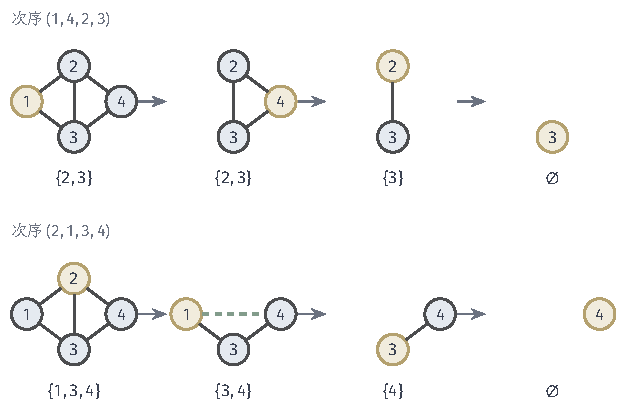
\includegraphics[width=105.004mm]{figures/01-basic-mathematics/04-graphs/tikz/c5-elimination-orders/figure.pdf}
  \caption{两种消元次序下原始图的变化。上行按$(1,4,2,3)$消元，每一步被消去的黄色顶点的邻居都已两两相邻，不产生填充边，新函数至多读取两个变量。下行按$(2,1,3,4)$消元，消去$2$时要补入填充边$\{1,4\}$（第二个图中的绿色虚线），新函数读取三个变量。每个图下方标出消去黄色顶点后新函数的作用域。}
  \label{fig:graph-dp-elimination-orders}
\end{figure}

第一种次序的最大中间表只有$4$项，第二种有$8$项。在这个小例子里差别不大；但若每个变量有$q$个状态，读取$r$个变量的表就有$q^r$项，多读取一个变量意味着表扩大$q$倍。

次序选得不好时，即使在树上也会产生大表：在第~\ref{sec:graph-dp-tree-messages}小节的分叉树上先消去中心$3$，它的邻居$1,2,4$两两补边，新函数要读取三个变量；而按后序消元时不产生任何填充边。两种次序算出的最小值相同（第~\ref{sec:graph-dp-min-cost-correctness}小节），差别只在中间表的规模。

\subsubsection{贪心规则}

定理~\ref{thm:graph-dp-treewidth-induced-width}把找好的树分解归结为找诱导宽度小的消元次序。在一般图上找诱导宽度最小的次序是困难的组合问题，实践中常用局部规则逐轮挑选顶点，得到一个可用但不保证最优的次序。

消去一个顶点，就是把它的全部当前邻居拉进同一个袋，并让它们两两相邻。代价因此体现在两处：它的当前邻居越多，这一步的袋越大；邻居之间缺的边越多，要补的填充边越多，剩下的图越稠密，以后的袋也可能越大。据此有两条常见规则：\term{最小度启发式}（min-degree），选当前邻居最少的顶点；\term{最小填充启发式}（min-fill），选消去时需要补边最少的顶点，即当前邻域中缺少的边数最少者。两条规则都只看当前这一步。

\paragraph{算法实现}

原图和评分规则在运行中不变。算法维护三项状态：
\begin{itemize}
  \item 当前图：初值为原图的副本；
  \item 已输出的次序：初值为空；
  \item 各轮的袋和填充边：初值为空。
\end{itemize}
每一轮依次做三件事：
\begin{itemize}
  \item 评分：在当前图上为每个剩余顶点计算评分，即当前度数或当前缺边数；
  \item 选择：取评分最小者，评分相同时取编号最小者，记为$v$；
  \item 消去：记录袋$\{v\}\cup N(v)$，其中$N(v)$是$v$的当前邻居，把$N(v)$补成团并记录填充边，删去$v$，把$v$追加到次序末尾。
\end{itemize}
当前图为空时停止。

\begin{algorithm}[贪心选择消元次序]
\label{alg:graph-dp-greedy-order}
输入：非空有限无向图和一条评分规则（当前度数或当前缺边数）。输出：消元次序、各轮的袋和填充边。
\begin{enumerate}
  \item 对当前图中的每个顶点按规则计算评分，取评分最小者，评分相同时取编号最小者，记为$v$。
  \item 记录袋$\{v\}\cup N(v)$，把$N(v)$补成团，删去$v$，并把$v$追加到次序末尾。
  \item 若图非空，回到第1步，并在更新后的图上重新计算评分。
\end{enumerate}
\end{algorithm}

评分必须在每轮更新后的图上重算。若只按初始度数排一次序，或用原图的缺边数代替当前缺边数，得到的就不是这两条规则，因为补边会改变其他顶点的度数和邻域。

\paragraph{执行过程}
图~\ref{fig:graph-dp-min-degree-min-fill}的图有六个顶点和边$\{1,3\},\allowbreak\{1,4\},\allowbreak\{1,5\},\allowbreak\{1,6\},\allowbreak\{2,3\},\allowbreak\{2,4\},\allowbreak\{2,6\},\allowbreak\{3,5\},\allowbreak\{4,5\},\allowbreak\{5,6\}$。初始度数依次为$4,3,3,3,4,3$；缺边数依次为$3,3,2,2,3,2$，例如顶点$2$的邻居$3,4,6$两两不相邻，缺$3$条边，而顶点$3$的邻居$1,2,5$中只缺$\{1,2\}$与$\{2,5\}$。表~\ref{tab:graph-dp-greedy-order-trace}并列两条规则的各轮结果。

最小度规则的执行如下：
\begin{itemize}
  \item 第$1$轮：度数为$3$的有$2,3,4,6$，按编号选$2$，袋为$\{2,3,4,6\}$，补入$\{3,4\},\allowbreak\{3,6\},\allowbreak\{4,6\}$。
  \item 第$2$轮：剩下的五个顶点因此两两相邻，度数都是$4$，按编号选$1$，袋为$\{1,3,4,5,6\}$，宽度升到$4$。
  \item 第$3$至$6$轮：剩余图始终是完全图，依次选$3,4,5,6$，不再补边。
\end{itemize}
最小填充规则的执行如下：
\begin{itemize}
  \item 第$1$轮：缺边数为$2$的有$3,4,6$，按编号选$3$，袋为$\{1,2,3,5\}$，补入$\{1,2\}$与$\{2,5\}$。
  \item 第$2$轮：$4$的邻居$1,2,5$已两两相邻，缺边数为$0$；$6$的缺边数也是$0$，按编号选$4$，袋为$\{1,2,4,5\}$。
  \item 第$3$至$6$轮：剩下的四个顶点两两相邻，依次选$1,2,5,6$，不再补边。
\end{itemize}
最大袋含$4$个顶点，宽度为$3$，比最小度规则少$1$。

\begin{table}[!htb]
  \centering
  \caption{两条贪心规则在图~\ref{fig:graph-dp-min-degree-min-fill}的六顶点图上的各轮结果。“选中”列括号内是该顶点当轮的评分（最小度规则为当前度数，最小填充规则为当前缺边数），“补边”列是该轮补入的填充边条数。}
  \label{tab:graph-dp-greedy-order-trace}
  \small
  \begin{tabular}{@{}ccccccc@{}}
    \toprule
    & \multicolumn{3}{c}{最小度} & \multicolumn{3}{c}{最小填充}\\
    \cmidrule(lr){2-4}\cmidrule(lr){5-7}
    轮 & 选中 & 袋 & 补边 & 选中 & 袋 & 补边\\
    \midrule
    $1$ & $2$（$3$） & $\{2,3,4,6\}$ & $3$ & $3$（$2$） & $\{1,2,3,5\}$ & $2$\\
    $2$ & $1$（$4$） & $\{1,3,4,5,6\}$ & $0$ & $4$（$0$） & $\{1,2,4,5\}$ & $0$\\
    $3$ & $3$（$3$） & $\{3,4,5,6\}$ & $0$ & $1$（$0$） & $\{1,2,5,6\}$ & $0$\\
    $4$ & $4$（$2$） & $\{4,5,6\}$ & $0$ & $2$（$0$） & $\{2,5,6\}$ & $0$\\
    $5$ & $5$（$1$） & $\{5,6\}$ & $0$ & $5$（$0$） & $\{5,6\}$ & $0$\\
    $6$ & $6$（$0$） & $\{6\}$ & $0$ & $6$（$0$） & $\{6\}$ & $0$\\
    \midrule
    宽度 & \multicolumn{3}{c}{$4$} & \multicolumn{3}{c}{$3$}\\
    \bottomrule
  \end{tabular}
\end{table}

\begin{figure}[!htb]
  \centering
  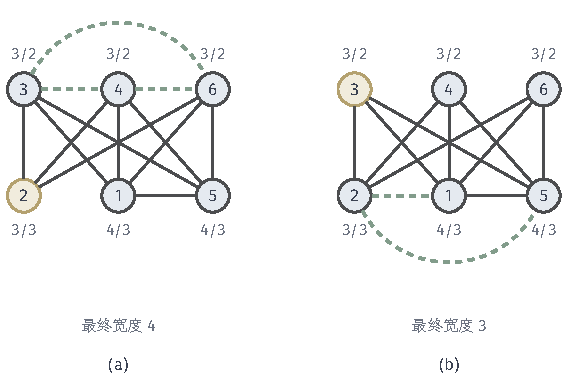
\includegraphics[width=96.778mm]{figures/01-basic-mathematics/04-graphs/tikz/c5-min-degree-min-fill/figure.pdf}
  \caption{最小度规则与最小填充规则的第一步。每个顶点旁的“$d/f$”是当前度数与当前缺边数。左：最小度规则在度数为$3$的顶点中按编号选$2$（黄色），要补三条绿色虚线，最终宽度为$4$。右：最小填充规则选缺边最少的$3$（黄色），只补两条边，最终宽度为$3$。}
  \label{fig:graph-dp-min-degree-min-fill}
\end{figure}

\subsubsection{贪心规则的分析}

\paragraph{启发式的局限}
两种规则都只看一步：度数小不代表补边少，补边少也不保证以后的袋小。上例中最小度规则受平局规则影响，第一步补的三条边把剩余图变成了完全图，得到的宽度比最小填充多$1$。穷举全部$720$个消元次序可以核对，这个图上任何次序的诱导宽度都不小于$3$，所以最小填充在这里恰好达到了最好的次序。换一个图，最小填充同样可能不是最优。因此报告结果时应分开写出构造的宽度、填充边数和结构操作次数，并把宽度理解为树宽的上界，而不是树宽本身。

宽度按变量个数计，而表的项数按状态数之积计。各变量状态数不同时，诱导宽度相同的两个次序，其最大消元簇的配置数可以相差很多；这时可以把评分换成消元簇上的状态数之积，或者构造后直接比较各簇的实际配置数。第~\ref{sec:graph-dp-table-size}小节按实际乘积比较候选结构。

\paragraph{复杂度}
直接实现时每轮要为全部剩余顶点重算评分。最小度规则的评分只需读出度数；最小填充规则要检查每个顶点的每对邻居是否相邻，一轮的检查量可达$\sum_v|N(v)|^2$。用缓存时只重算受影响的顶点：加入边$\{a,b\}$只改变$a$、$b$及其公共邻居的评分，删去$v$只改变$v$的邻居的评分。

\subsection{弦图与完美消元序}
\label{sec:graph-dp-chordal}

填充边会使袋变大，最理想的情形是全程不需要补边。处理顶点$v$时不需要补边，当且仅当$v$的当前邻居已经两两相邻。当前邻居构成团的顶点称为\term{单纯顶点}（simplicial vertex）；没有邻居或只有一个邻居的顶点也算单纯顶点。若一个消元次序使每个顶点在被处理时都是当前图中的单纯顶点，就称它为\term{完美消元序}（perfect elimination ordering）。沿完美消元序消元不产生任何填充边，当前图始终是原图在剩余顶点上的诱导子图。

\paragraph{弦图}
不是每个图都有完美消元序。四个顶点的环$1-2-3-4-1$中，每个顶点的两个邻居都不相邻：$1$与$3$的邻居都是$\{2,4\}$，缺边$\{2,4\}$；$2$与$4$的邻居都是$\{1,3\}$，缺边$\{1,3\}$。所以第一步就找不到单纯顶点。补入边$\{1,3\}$后，顶点$2$的邻居$\{1,3\}$相邻，可以先消去；剩下的三角形$1,3,4$中每个顶点都单纯，于是$(2,1,3,4)$是完美消元序。图~\ref{fig:graph-dp-chordal-four-cycle}画出了这一对比。

\begin{figure}[!htb]
  \centering
  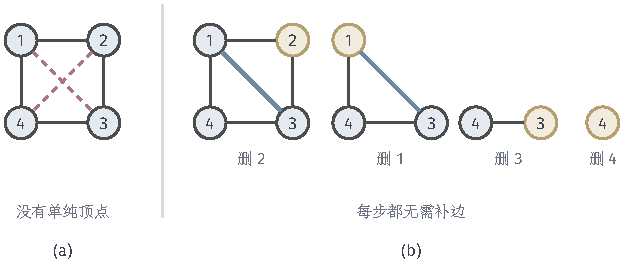
\includegraphics[width=106.306mm]{figures/01-basic-mathematics/04-graphs/tikz/c5-chordal-four-cycle/figure.pdf}
  \caption{无弦四环与补弦后的图。左：四环中每个顶点的两个邻居都不相邻（红色虚线为所缺的边），没有单纯顶点。右：补入弦$\{1,3\}$（蓝色）后，按$(2,1,3,4)$逐个删除，每一步被删除的黄色顶点的剩余邻居都已相邻，全程无填充。}
  \label{fig:graph-dp-chordal-four-cycle}
\end{figure}

四环的问题出在“长度至少为四而没有捷径的环”。消去这种环上的任何一个顶点，它在环上的两个邻居都不相邻，必须补一条边把它们直接连起来；三角形则没有这个问题，因为两个邻居本来就相邻。在长度至少为$4$的环上，连接两个在环上不相邻的顶点的边称为该环的\term{弦}（chord），也就是一条捷径。每个长度至少为$4$的环都有弦的有限无向图称为\term{弦图}（chordal graph）。

树没有环，是弦图；补入$\{1,3\}$后的四环是弦图；无弦四环不是。给一般图补边使之成为弦图称为\term{弦化}（chordal completion）。

\begin{theorem}[弦图与完美消元序]
\label{thm:graph-dp-chordal-peo}
有限无向图是弦图，当且仅当它有完美消元序。
\end{theorem}

\begin{proof}
先证有完美消元序的图是弦图。设图中有长度至少为$4$且无弦的环，考察环上最先被处理的顶点$v$。$v$在环上的两个邻居$u,w$此时都还在图中，并且与$v$相邻。$v$是单纯顶点，所以$u,w$相邻；而沿完美消元序处理时从不补边，$\{u,w\}$必是原图的边。环长至少为$4$，$u,w$在环上不相邻，于是$\{u,w\}$是这个环的弦，矛盾。

反方向的论证路线如下。第一步是一个引理：每个非空有限弦图都有单纯顶点，若它不是完全图，还有两个不相邻的单纯顶点。这一步需要分析极小分隔集，证明极小分隔集在弦图中都是团，本书不展开。第二步，弦图的诱导子图仍是弦图，因为诱导子图中的无弦环在原图中也无弦。于是可以反复删去一个单纯顶点，余下的图仍是弦图、仍有单纯顶点，直到删完，删除的次序就是完美消元序。
\end{proof}

\paragraph{填充图与弦化}
一般图经一次完整消元得到的填充图$\mathcal G^+_\pi$（第~\ref{sec:graph-dp-fill-in}小节）总是弦图，并且$\pi$就是它的完美消元序。要验证这一点，只需说明在$\mathcal G^+_\pi$中，$v$排在它之后的邻居恰是消元时的剩余邻居$N^+_\pi(v)$：$\mathcal G^+_\pi$中连接$v$与某个较晚顶点$w$的边，若是原始边，处理$v$时仍在；若是填充边，它在处理某个更早的顶点时补入，那时$v$还没有被删去，所以处理$v$时这条边也在。于是这些后续邻居在处理$v$时已被补成团，$v$在$\mathcal G^+_\pi$中按$\pi$处理时总是单纯顶点。由定理~\ref{thm:graph-dp-chordal-peo}，$\mathcal G^+_\pi$是弦图，第~\ref{sec:graph-dp-order-to-decomposition}小节的构造实际上隐含了一次弦化。

反过来，设$\mathcal H$是包含$\mathcal G$的弦图（顶点相同、边更多），$\sigma$是$\mathcal H$的完美消元序。按$\sigma$对$\mathcal G$消元，对步数归纳可知当前图始终是$\mathcal H$在剩余顶点上的诱导子图的子图：处理$v$时，它的当前邻居包含在$\mathcal H$中$v$的后续邻居里，后者在$\mathcal H$中成团，所以补入的填充边都是$\mathcal H$的边。因此$\mathcal G^+_\sigma\subseteq\mathcal H$，每个消元簇都含于$\mathcal H$的某个团，诱导宽度不超过$\mathcal H$的最大团大小减一。

这样，消元次序与弦化相互对应：选一个次序就选定了一个弦化，选一个弦化及其完美消元序也就得到一个宽度不更大的次序。四环算例按$(1,2,3,4)$消元，填充图是环加上弦$\{2,4\}$，$(1,2,3,4)$正是它的完美消元序；按$(2,1,3,4)$消元则对应图~\ref{fig:graph-dp-chordal-four-cycle}中补弦$\{1,3\}$的弦化。

\subsection{完美消元序的构造与核验}
\label{sec:graph-dp-peo-construction}

\subsubsection{问题与思路}

定理~\ref{thm:graph-dp-chordal-peo}只说明弦图有完美消元序，没有给出求法。输入是一个有限无向图，输出是它的一个完美消元序，或者“不是弦图”的报告及证据。定理证明的反方向已经提示了做法：反复找一个单纯顶点删去。弦图的每个诱导子图仍有单纯顶点，所以对弦图这一过程不会卡住；非弦图没有完美消元序，过程必然在某一轮找不到单纯顶点，这时剩下的图本身就是证据。

\subsubsection{算法实现}

输入图在运行中不变。算法维护两项状态：
\begin{itemize}
  \item 当前图：初值为输入图的副本；
  \item 已输出的次序：初值为空。
\end{itemize}
每一轮依次做两件事：
\begin{itemize}
  \item 检查：按编号逐个检查当前图中的顶点，枚举它的每对邻居看是否相邻，遇到第一个单纯顶点就停下；
  \item 删除：把找到的单纯顶点从当前图中删去，追加到次序末尾。
\end{itemize}
当前图为空时停止，输出的次序就是完美消元序。若非空的当前图中找不到单纯顶点，就停止并报告输入不是弦图，返回这个当前图作为证据，而不暗中补边。

\begin{algorithm}[逐次删除单纯顶点]
\label{alg:graph-dp-peo-construction}
输入：有限无向图。输出：完美消元序，或“不是弦图”的报告及当前图。
\begin{enumerate}
  \item 令当前图为输入图的副本，次序为空。
  \item 若当前图为空，输出次序并停止。
  \item 按编号检查当前图的顶点，找出第一个邻居两两相邻的顶点$v$；若不存在，报告输入不是弦图，返回当前图并停止。
  \item 从当前图中删去$v$，把$v$追加到次序末尾，回到第2步。
\end{enumerate}
\end{algorithm}

\paragraph{执行过程}
在补弦后的四环上（边$\{1,2\},\allowbreak\{2,3\},\allowbreak\{3,4\},\allowbreak\{1,4\},\allowbreak\{1,3\}$）：
\begin{itemize}
  \item 第$1$轮：顶点$1$的邻居$\{2,3,4\}$缺边$\{2,4\}$，跳过；顶点$2$的邻居$\{1,3\}$相邻，选中并删去。
  \item 第$2$轮：剩下三角形$1,3,4$，顶点$1$的邻居$\{3,4\}$相邻，选中。
  \item 第$3$、$4$轮：依次选中$3$与$4$。
\end{itemize}
输出$(2,1,3,4)$。在无弦四环上，第$1$轮四个顶点都不单纯，过程失败并返回整个四环。

\subsubsection{算法分析}

\paragraph{正确性}
成功时，每个顶点在被删去时都是当前图的单纯顶点，而删点不补边，当前图始终是输入图的诱导子图，所以输出的次序是完美消元序。对弦图，由定理~\ref{thm:graph-dp-chordal-peo}证明中的引理与诱导子图的封闭性，每一轮的当前图都有单纯顶点，过程不会中途失败；对非弦图，若过程成功就得到一个完美消元序，与定理矛盾，所以必然在某一轮失败。

\paragraph{复杂度}
直接实现每轮最多检查$n$个顶点，检查顶点$v$需要$O(|N(v)|^2)$次查边，总检查量最坏可达$O(n^4)$。存在线性时间的专门算法，这里不展开。

\subsubsection{完美消元序的核验}

构造得到的次序应当独立核验，来自别处的次序更应如此。给定原图和一个次序，按下面的步骤检查：
\begin{itemize}
  \item 确认次序恰好包含每个顶点一次，并为每个顶点记下次序位置；
  \item 对每个$v$取出原图中排在它之后的邻居，检查它们是否两两相邻。
\end{itemize}
全部通过时次序是完美消元序，因为在不补边的前提下，处理$v$时的当前邻居恰好就是这些后续邻居；发现缺边时，就把$v$和那对不相邻的邻居作为失败证据返回。例如把$(2,1,3,4)$用于无弦四环，第一个顶点$2$的后续邻居$\{1,3\}$不相邻，立即被拒绝；用于补弦后的图则通过。

核验只需$O(n+m)$再加$\sum_v|N^+_\pi(v)|^2$次查边，比构造便宜得多，所以即使次序来自别处，也值得先核验再使用。

\subsection{团树的构造}
\label{sec:graph-dp-clique-tree}

\subsubsection{问题与思路}

弦图上可以直接用团作袋，这需要区分两种“最大”。不能再加入任何其他顶点而保持两两相邻的团称为\term{极大团}（maximal clique），这是按集合包含判断的；在所有团中顶点数最多的称为\term{最大团}（maximum clique）。例如三角形$1,2,3$外加一条边$\{3,4\}$，极大团是$\{1,2,3\}$和$\{3,4\}$；后者不能再扩大，但只有两个顶点，不是最大团。以弦图的全部极大团为袋、并满足运行交集的树分解称为\term{团树}（junction tree，也称clique tree）。团树中每个袋都是团，没有因填充而多出的变量，相邻两袋的交集就是它们共享的变量。

给定一个弦图，构造团树要做两件事：得到全部极大团，再把它们连成满足运行交集的树。极大团可以从完美消元序中读出。设$\pi$是完美消元序，候选集合$K_v=\{v\}\cup N^+_\pi(v)$就是第~\ref{sec:graph-dp-order-to-decomposition}小节构造中的袋；$v$被处理时是单纯顶点，所以$K_v$是团，极大团就藏在这些候选中。

连接时要选一棵树，使每个变量所在的团连成一片。可以按变量数边：一个变量属于$r$个团时，树中两端都含它的边至多有$r-1$条，再多就会在这$r$个团之间成环；恰有$r-1$条时，这$r$个团才连成一片。反过来看一条树边$\{C,D\}$，它为$C\cap D$中的每个变量各计一条，所以它的贡献是$|C\cap D|$。以交集大小为边权，一棵生成树的总权就等于各变量的这种边数之和，不超过各变量的$r-1$之和；达到这个上限，恰好意味着每个变量的团都连成了一片。这样，连接团的问题变成了最大权生成树问题。把每条边的权取负，就可以直接调用第~\ref{chap:minimum-spanning-tree}章的最小生成树算法，那里的割性质保证Kruskal与Prim方法给出最优树。

\subsubsection{算法实现}

输入是弦图$\mathcal H$，先用第~\ref{sec:graph-dp-peo-construction}小节的方法求出并核验它的完美消元序$\pi$；此后$\mathcal H$与$\pi$都不再改变。算法维护三项状态：
\begin{itemize}
  \item 团表：初值为全部候选$K_v$，处理后只剩极大团；
  \item 候选边表：团两两之间的边及其权$w(C,D)=|C\cap D|$，按权从大到小排列；
  \item 并查集与已选树边：并查集初值为每个团各成一组，已选树边初值为空。
\end{itemize}
计算分三步：
\begin{itemize}
  \item 求极大团：对每个顶点生成候选$K_v$，删去重复的集合和被其他候选严格包含的集合，剩下的就是全部极大团。
  \item 连接：在以极大团为顶点的完全图上，按权从大到小考察候选边，两端不在同一组时加入树边并合并两组，否则跳过；这正是把权取负后调用Kruskal方法：负权的最小生成树就是原权的最大权生成树。也可以改用Prim方法。
  \item 核验：对输出的树逐个顶点检查运行交集。
\end{itemize}
已选树边达到团数减一时，连接停止。

\begin{algorithm}[由弦图构造团树]
\label{alg:graph-dp-clique-tree}
输入：有限弦图$\mathcal H$。输出：$\mathcal H$的团树。
\begin{enumerate}
  \item 求完美消元序$\pi$并核验；对每个顶点$v$生成候选$K_v=\{v\}\cup N^+_\pi(v)$。
  \item 删去重复的候选和被其他候选严格包含的候选，得到极大团$\mathcal C$。
  \item 对$\mathcal C$中每对团计算$w(C,D)=|C\cap D|$，按权从大到小考察，用并查集判断是否成环，不成环时加入树边，直到树边数为$|\mathcal C|-1$。
  \item 对每个顶点检查含它的团在树中是否连通。
\end{enumerate}
\end{algorithm}

\paragraph{执行过程}
图~\ref{fig:graph-dp-clique-tree-mst}的弦图有边$\{1,2\},\allowbreak\{1,3\},\allowbreak\{2,3\},\allowbreak\{2,4\},\allowbreak\{3,4\},\allowbreak\{3,5\},\allowbreak\{4,5\}$。
\begin{itemize}
  \item 完美消元序：取$(1,2,5,3,4)$并核验，各顶点在次序中靠后的邻居分别为$\{2,3\}$、$\{3,4\}$、$\{3,4\}$、$\{4\}$、$\varnothing$，都两两相邻。
  \item 求极大团：候选为$K_1=\{1,2,3\}$、$K_2=\{2,3,4\}$、$K_5=\{3,4,5\}$、$K_3=\{3,4\}$、$K_4=\{4\}$；$K_3$被$K_2$包含，$K_4$被$K_3$包含，删去后得到三个极大团$A=\{1,2,3\}$、$B=\{2,3,4\}$、$C=\{3,4,5\}$。
  \item 计算权：$w(A,B)=|\{2,3\}|=2$、$w(B,C)=|\{3,4\}|=2$、$w(A,C)=|\{3\}|=1$。
  \item 连接：先加入$A-B$，再加入$B-C$，此时三个团已连通，$A-C$会成环而被跳过。得到的最大权生成树是$A-B-C$，总权为$4$。
  \item 核验：含$3$的团$A,B,C$沿$A-B-C$连通，含$2$的团$A,B$相邻，含$4$的团$B,C$相邻，运行交集成立。
\end{itemize}
若改选$A-B$与$A-C$，总权为$3$，此时含$4$的两个团$B,C$之间隔着不含$4$的$A$，运行交集被破坏，如图~\ref{fig:graph-dp-clique-tree-mst}右侧所示。

\begin{figure}[!htb]
  \centering
  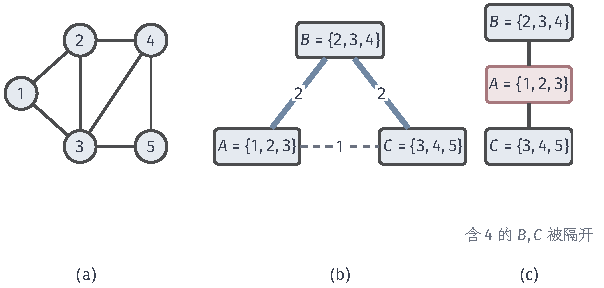
\includegraphics[width=102.306mm]{figures/01-basic-mathematics/04-graphs/tikz/c5-clique-tree-mst/figure.pdf}
  \caption{用交集权重的最大权生成树连接极大团。左：弦图。中：三个极大团组成的候选完全图，边上的数是交集大小，蓝色粗线是总权为$4$的最大权生成树$A-B-C$，虚线是未被选中的候选边。右：总权为$3$的另一棵生成树$B-A-C$，含$4$的团$B,C$被不含$4$的$A$（红色）隔开，不满足运行交集。}
  \label{fig:graph-dp-clique-tree-mst}
\end{figure}

\subsubsection{算法分析}

\paragraph{正确性}
先说明候选集合给出全部极大团。每个$K_v$都是团。反过来，任一团$C$都包含在某个$K_v$中：取$C$中最先被处理的顶点$v$，$C$的其余顶点都在$v$之后且与$v$相邻；沿完美消元序消元不补边也不删去尚未处理的顶点之间的边，它们在处理$v$时仍是$v$的当前邻居，所以都属于$N^+_\pi(v)$。因此每个极大团都等于某个$K_v$（它包含于某个团$K_v$，又是极大的），而不被其他候选严格包含的候选都是极大团。这也说明弦图的极大团数不超过顶点数$n$。

上面的例子中，满足运行交集的树恰好是总权最大的树。下面的定理把思路中的计数写成证明，说明这一对应是一般的。

\begin{theorem}[团树与最大权生成树]
\label{thm:graph-dp-clique-tree-mst}
设$\mathcal H$是非空有限弦图，$\mathcal C$是它的全部极大团。在以$\mathcal C$为顶点的完全图上令$w(C,D)=|C\cap D|$。则一棵生成树满足运行交集，当且仅当它的总权最大。
\end{theorem}

\begin{proof}
先给出任意生成树的总权上界。对生成树$\mathcal T'$，把每条边的权按共享变量拆开计数：
\[
\sum_{\{C,D\}\in\mathcal T'}|C\cap D|=\sum_{v}e_v,
\]
其中$e_v$是两端都含$v$的树边条数。设$v$属于$r_v$个极大团，两端都含$v$的树边正是$\mathcal T'$在这$r_v$个节点上的诱导子图的边；树的诱导子图没有环，是$r_v$个节点上的森林，所以$e_v\leq r_v-1$，且等号成立当且仅当这个诱导子图连通，即含$v$的团在$\mathcal T'$中连通。于是总权不超过$\sum_v(r_v-1)$，等号成立当且仅当对每个$v$都满足运行交集。

剩下要证明确实存在满足运行交集的生成树，即团树存在；那时最大总权恰为$\sum_v(r_v-1)$，最大权生成树就是满足运行交集的生成树。取一个完美消元序，按定理~\ref{thm:graph-dp-elimination-decomposition}的方法以$K_v$为袋得到树分解。若某个袋包含于相邻的袋，就把这条袋树边收缩，只保留较大的袋：顶点覆盖和边覆盖不受影响；对运行交集，被收缩的较小袋中的变量都在较大袋中，收缩一条两端都含$v$的边不破坏$T_v$的连通性，而不含$v$的较小袋本来不在$T_v$中，收缩后$T_v$也不变。

反复收缩，直到没有相邻两袋有包含关系。这时任何两个袋都没有包含关系：若$B_s\subseteq B_t$而$s,t$不相邻，取路径上与$s$相邻的节点$s'$，由运行交集$B_s$的每个变量都在$B_{s'}$中，与“相邻袋无包含关系”矛盾。各袋都是团且互不包含；每个极大团都被某个袋容纳（引理~\ref{lem:graph-dp-clique-in-bag}），而袋本身是团，所以二者相等；每个袋也都是某个极大团，否则它会被那个极大团所在的另一个袋严格包含。于是剩下的袋恰好是全部极大团，各出现一次，团树存在。
\end{proof}

在上例中，$r_1=1$、$r_2=2$、$r_3=3$、$r_4=2$、$r_5=1$，上界$\sum_v(r_v-1)=4$，正好等于$A-B-C$的总权。不连通的弦图中，不同分量的团之间交集为空，零权边只用于把各分量的团树连成一棵树，不影响上界。上面的计数也给出了最后一步核验的做法：检查每个$e_v$是否等于$r_v-1$。

\paragraph{复杂度}
设极大团有$p\leq n$个，候选完全图有$p(p-1)/2$条边，每条边的权需要一次集合求交，排序与并查集的开销按第~\ref{chap:minimum-spanning-tree}章的分析计算。求完美消元序和候选集合的开销见第~\ref{sec:graph-dp-peo-construction}小节与第~\ref{sec:graph-dp-order-to-decomposition}小节。

\paragraph{适用范围}
定理要求输入是弦图，并且使用全部极大团。对无弦四环，极大团是四条边$\{1,2\},\allowbreak\{2,3\},\allowbreak\{3,4\},\allowbreak\{1,4\}$，每个顶点属于两个团；要让每个顶点的两个团相邻，需要四条树边，而四个节点的树只有三条边，所以任何生成树都不满足运行交集。一般图应先弦化，例如用某个消元次序补边，再在弦化后的图上构造团树；在原图的极大团上任选一棵树并不能保证得到树分解。选哪一种弦化决定了袋的大小，而团树构造只负责连接给定弦图的团，不负责找最好的弦化。输出后逐个顶点检查运行交集，也是对输入是否为弦图、团列表是否完整的独立核对。

\subsection{构建结果的检验}
\label{sec:graph-dp-construction-check}

无论结构来自消元次序、贪心规则还是团树构造，交给下一章计算之前都应独立检验。检验只读输出的袋树，不依赖它是怎样构造出来的，所以同样适用于来自别处的分解。检验的对象是原始图$\mathcal G$（有保留集时是$\mathcal G_R$）、局部函数的作用域、袋树及选定的根。

\paragraph{树分解的三个条件}
核验按定义逐条进行：确认袋树是树，即节点数减一等于边数且连通；扫描各袋得到每个顶点的$T_v$，检查顶点覆盖与边覆盖；对每个顶点$v$数出两端袋都含$v$的袋树边条数$e_v$。这些边恰是树在$T_v$上的诱导子图的边，而树的诱导子图是森林，所以$e_v\leq|T_v|-1$，等号成立当且仅当$T_v$连通。

图~\ref{fig:graph-dp-running-intersection}下面的连接中$|T_2|=2$而$e_2=0$，核验失败，$2$就是失败的证据；梯子的分解中$|T_2|=3$、$e_2=2$，通过。团树构造中的最后一步核验（检查每个$e_v$是否等于$r_v-1$）也是这一检查。

\paragraph{作用域、接口与查询}
树分解的条件只涉及原始图的边。计算还需要每个局部函数有处可放，所以对每个作用域$S_a$找出一个包含它的袋并记录下来；引理~\ref{lem:graph-dp-clique-in-bag}保证合法的分解总能通过这项检查，找不到时说明分解本身有误或作用域与原始图不符。

选定根以后，为每个非根节点算出接口$S_u=B_u\cap B_{p(u)}$与内部变量$I_u$，并核对每个变量恰在一个节点作内部变量（引理~\ref{lem:graph-dp-unique-internal}）。有保留集$R$时，另检查根袋包含$R$。最后记录实际宽度，以及各袋、各接口上的状态数之积，供第~\ref{sec:graph-dp-computation-cost}节估计代价。

\paragraph{检验的代价}
设袋树有$N$个节点，各袋大小之和为$L=\sum_t|B_t|$。建立每个顶点的$T_v$和数出各$e_v$需要扫描各袋及各条袋树边两端的公共变量，时间为$O(L+n)$量级（用以变量为下标的数组标记袋内成员）；边覆盖与作用域容纳的检查对每条边或每个作用域，在最小的$T_v$中逐袋测试包含关系。这些都是关于袋大小的多项式开销，与随状态数指数增长的数值计算相比通常很小，但它们是构建阶段的成本，应与构造本身的成本分开记录，不计入下一章的求值时间。

四环算例的分解$\{1,2,4\}-\{2,3,4\}$以$\{2,3,4\}$为根时，检验结果为：四条边分别被两个袋覆盖；$e_2=e_4=1=|T_2|-1=|T_4|-1$，$e_1=e_3=0=|T_1|-1=|T_3|-1$；四个作用域$\{1,2\},\{1,4\}$放进第一个袋，$\{2,3\},\{3,4\}$放进根袋；子节点的接口为$\{2,4\}$、内部变量为$\{1\}$，根的内部变量为$\{2,3,4\}$；宽度为$2$，每个袋上有$8$种配置，接口上有$4$种。

\FloatBarrier
\section{本章小结}
\label{sec:dp-construction-chapter-summary}

本章回答的是：在计算任何数值之前，一般图上的动态规划要把哪些变量放在一起处理、以哪些变量为接口、按什么次序传递结果。构建的输入只是作用域，所得结构对作用域相同而数值任意的全部问题都适用；一般数值下必须保留的耦合一律保留，不利用特定数值的巧合。

合法的结构是原始图的树分解。顶点覆盖和边覆盖保证每个变量、每条边有处可放，而由两两相交子树的公共节点可知，每个作用域乃至每个团都被某个袋整体容纳；运行交集保证每个变量在袋树上占据连成一片的地盘，于是接口把两侧的变量和局部项隔开，以接口为索引的摘要不会丢失信息。选根以后，每个变量恰在它所在的最高节点作内部变量，所以每个变量恰被汇总一次。带保留变量的查询要先把保留集补成团，并选包含它的袋作根，宽度要按补边后的图计算。

变量消元与树分解是同一结构的两种描述。按次序在原始图上模拟消元，填充边记录新产生的耦合，消元簇连到其剩余作用域中最早被消去的变量的袋，就得到树分解，每个非根袋的接口恰是该步中间函数的作用域；反过来，从叶袋向内消去只出现在叶袋中的变量，就读出诱导宽度不超过分解宽度的次序。两个方向合起来，树宽等于最小诱导宽度；但某个具体次序或分解的宽度只是上界，二者也不一一对应。

实际构造时，最小度、最小填充等贪心规则给出可用但不保证最优的次序，状态数不同时还要比较实际的配置数；每个消元次序都隐含一次弦化，弦图有不需补边的完美消元序，可以逐次删除单纯顶点来构造并独立核验；弦图的极大团以交集大小为权、经最大权生成树连成团树。构建结果在交付计算前逐项检验三个条件、作用域容纳、接口与查询根，并记录实际宽度与状态数之积。数值表怎样在这样的结构上计算、怎样恢复配置、代价多大，由下一章回答。


\chapter{一般图上动态规划的计算}
\label{sec:graph-bag-dp}
\label{chap:general-graph-dp-computation}

上一章构建并核验了计算所需的结构：袋树、选定的根、每个节点的接口与内部变量；有查询时，根袋还包含保留集。本章在这个结构上填写数值表，回答第~\ref{sec:graph-dp-problem}小节提出的几种任务：最小成本及一个最优配置，保留一组变量时的条件最小成本表，可行配置的个数，以及非负权重之积的总和。对每种任务，我们说明输入、输出、递推与正确性，并用算例检验；最后分析这些计算实际需要多少时间和存储。

各任务共用同一套组织方式，第~\ref{sec:graph-dp-assignment-order}节先把它固定下来：每个局部项恰好归入一个容纳其作用域的袋，按后序由叶到根处理，并说明按消元次序计算与沿袋树计算得到同样的中间函数。

第~\ref{sec:graph-dp-min-cost}节处理最小成本。每个袋把本地成本与子袋消息相加，对内部变量取最小，再把结果沿接口交给父袋；取最小时记下达到值的内部取值，根选定最优状态后沿袋树恢复配置。正确性归结为一个不变量：消息等于固定接口后下方全部局部项之和的最小值。第~\ref{sec:graph-dp-retained-min}节保留一组变量，只在根袋中对其余变量取最小，得到以保留变量为索引的表。

第~\ref{sec:graph-dp-semiring}节把相加换成相乘、取最小换成求和，计算可行配置数和加权总和，并说明求和与取最小不能随意交换次序。第~\ref{sec:graph-dp-computation-cost}节把袋与接口换算成实际的表项数，分析时间、存储及二者的取舍。

本章沿用第~\ref{sec:graph-dp-four-cycle}小节的四环算例，并用第~\ref{chap:local-functions-tree-dp}章的三元作用域例子演示消元的逐步过程；两例都可以与枚举结果逐项核对。

% 第13章第1节：局部项归属与求值顺序（局部项的唯一归属、选根与求值顺序、消元与袋树的求值对应）。

\section{局部项归属与求值顺序}
\label{sec:graph-dp-assignment-order}

在填写任何数值之前，要先固定两件事：每个局部项由哪个袋负责，以及各袋按什么顺序计算。这两件事对本章所有任务都相同。先把它们固定下来，既能避免重复计入局部项，也能保证比较两种表示时计算的是同一个对象。

\subsection{局部项的唯一归属}
\label{sec:graph-dp-term-assignment}

计算前先把每个局部函数$\phi_a$归入一个袋$B_{\alpha(a)}$，要求$S_a\subseteq B_{\alpha(a)}$；由引理~\ref{lem:graph-dp-clique-in-bag}，这样的袋总存在。映射$\alpha:A\to T$称为局部项的归属。记归入节点$u$的局部项集合为$A_u=\{a:\alpha(a)=u\}$，它们的和
\begin{equation}
\Phi_u(\bm x_{B_u})=\sum_{a\in A_u}\phi_a(\bm x_{S_a})
\label{eq:graph-dp-bag-cost}
\end{equation}
称为$u$的本地成本。没有局部项归入的袋取$\Phi_u\equiv0$（空和为$0$），但仍保留袋中的变量，因为它们可能需要经过这个袋来保持一致。计数和求和任务把相加换成相乘，空乘积取$1$，第~\ref{sec:graph-dp-semiring}节再说明。

只归入一次是数值正确性的要求。在三元作用域例子的分解$\{1,2,3\}-\{2,3,4\}$中，若另有成对项$\phi_{2,3}(x_2,x_3)$，它可以归入任一袋，但两边各计一次就会求出$F+\phi_{2,3}$的最小值。共享变量可以在多个袋中重复出现，同一个成本项却只能计一次；袋之间的交集本身不对应任何成本。计算前应逐项检查分配清单：无遗漏、无重复、作用域包含于所归的袋。

图~\ref{fig:graph-dp-single-factor-owner}把变量共享与函数归属分开表示。两个袋都保留$2,3$，但$\phi_{2,3}$只沿一条归属箭头进入左袋；把它改归右袋也合法，同时归入两袋则会重复计费。

\begin{figure}[!htb]
  \centering
  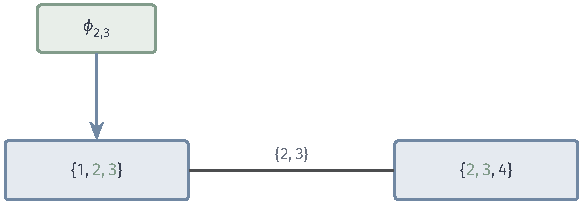
\includegraphics[width=98.651mm]{figures/03-graphs/04-local-functions-and-dynamic-programming/tikz/dp-single-factor-owner/figure.pdf}
  \caption{共享变量不意味着重复计入局部项。两个袋均包含$\phi_{2,3}$的作用域，图中选择左袋作为唯一归属。袋树横边仅表示接口连接，向下的蓝色箭头表示局部项归属，二者含义不同。}
  \label{fig:graph-dp-single-factor-owner}
\end{figure}

\paragraph{消元表示中的归属}
用消元森林表示结构时，归属有一条自然的规则：把$\phi_a$归入$S_a$中最早被消去的变量所对应的袋。第~\ref{sec:graph-dp-clusters-to-decomposition}小节已经说明这个袋包含$S_a$。这条规则恰好对应消元的实际过程：$\phi_a$在它的某个变量第一次被消去时被取出。作用域全在保留集$R$内的局部项（包括作用域为空的常数项）在消元中从不被取出，归入根袋；没有保留集时，常数项可归入任一个根袋。

在四环算例的分解$\{1,2,4\}-\{2,3,4\}$中，$\phi_{1,2}$与$\phi_{1,4}$只能归入$\{1,2,4\}$，$\phi_{2,3}$与$\phi_{3,4}$只能归入$\{2,3,4\}$。按次序$(1,2,3,4)$的消元森林来看，$\phi_{3,4}$本应归入$B_3=\{3,4\}$，这个袋并入$\{2,3,4\}$后归属随之并入。

三元作用域例子的分解中，$\phi_A$只能归入$\{1,2,3\}$，$\phi_B$只能归入$\{2,3,4\}$。

\subsection{选根与求值顺序}
\label{sec:graph-dp-root-order}

给已核验的袋树选根$r$，确定每个非根节点$u$的父节点$p(u)$、子节点集合$\operatorname{ch}(u)$、接口$S_u=B_u\cap B_{p(u)}$与内部变量$I_u=B_u\setminus S_u$（第~\ref{sec:graph-dp-interface-internal}小节）。查询任务使用第~\ref{sec:graph-dp-query-structure}小节保证覆盖保留集$R$的根袋。

求值按袋树的一个后序进行：先处理全部子节点，再处理父节点，最后处理根。每个非根节点只用到子节点交来的表，处理完后把一张以$\bm x_{S_u}$为索引的表交给父节点。后序可以由一次深度优先遍历的完成次序得到，它与根、父节点一样只规定处理次序，在运行中不变。需要恢复配置时，再按前序（后序的逆序，父节点总在子节点之前）走一遍。

原始图不连通时，各分量的袋树之间只有空接口的边相连。沿空接口传递的表只有一项，是一个数：最小成本任务中它是那个分量的最小成本，计数和求和任务中它是那个分量的总数或总和。根把收到的这些数与本分量的结果组合起来，组合方式随任务而定，在各任务中分别说明。

\paragraph{表的存储与对齐}
本地成本、消息和回溯表都是以一组变量为索引的稠密表。为每张表固定变量的排列（例如按编号），各取值按字典序存放，即$(x_{j_1},\ldots,x_{j_k})$像多位数一样以最后一个变量为最低位递增。于是一组取值的位置可以按混合进制直接算出，读取一项按常数时间计；本部分例子中的表都按这种次序列出，例如作用域为$\{2,4\}$的表依次对应$(x_2,x_4)=(0,0),(0,1),(1,0),(1,1)$。

计算时要在袋$B_u$的一组取值$\bm x_{B_u}$上读取$\phi_a(\bm x_{S_a})$或子节点的消息，即从$\bm x_{B_u}$中挑出$S_a$或$S_c$的那几个分量，再算它们在小表中的位置。各变量在$B_u$中的位置事先记下，每次读取就只需几次乘加。接口上的“对齐”指的正是这一步：发送方和接收方按同一组接口变量、同一排列存取消息。

\subsection{消元与袋树的求值对应}
\label{sec:graph-dp-elimination-message-correspondence}

第~\ref{sec:graph-dp-function-message-correspondence}小节在结构上对应了消元簇与袋、剩余作用域与接口。现在在数值上验证这一对应。沿袋树计算时，非根节点$u$先把本地成本与子节点的消息相加，得到
\[
g_u(\bm x_{B_u})=\Phi_u(\bm x_{B_u})+\sum_{c\in\operatorname{ch}(u)}m_{c\to u}(\bm x_{S_c}),
\]
再对内部变量取最小，得到发往父节点的消息
\[
m_{u\to p(u)}(\bm x_{S_u})=\min_{\bm x_{I_u}}g_u(\bm x_{B_u}).
\]
第~\ref{sec:graph-dp-min-cost}节逐项解释这两步。

\begin{theorem}[消元中间函数等于袋消息]
\label{thm:graph-dp-elimination-equals-messages}
设$\pi=(v_1,\ldots,v_k)$是$V\setminus R$的消元次序，袋树由算法~\ref{alg:graph-dp-order-to-decomposition}得到并以消元森林的根（有保留集时为$B_R$）为根，局部项按“作用域中最早被消去的变量”归属，作用域含于$R$的项归入根袋。则按次序消元时，第$i$步取出的函数恰为$\{\phi_a:a\in A_{B_i}\}$与$\{\psi_j:B_j\text{的父袋是}B_i\}$，并且$\psi_i=m_{B_i\to p(B_i)}$。
\end{theorem}

\begin{proof}
消元过程中，当前函数集合里的每个函数，作用域只含尚未消去的变量；它在作用域中第一个变量被消去时被取出，此前一直不动。原始局部项$\phi_a$因此在$S_a$中最早被消去的变量那一步被取出，这正是它的归属。中间函数$\psi_j$的作用域是$S_j$，它在$S_j$中最早被消去的变量那一步被取出，这正是$B_j$的父袋；若$S_j\subseteq R$，它从不被取出，最后留在根袋。这就证明了第一个断言。

再对$i$归纳证明$\psi_i=m_{B_i\to p(B_i)}$。第$i$步取出的函数之和为$\Phi_{B_i}$加上各子袋的$\psi_j$；由归纳假设，后者等于子袋发来的消息，所以这个和就是$g_{B_i}$。$B_i$的内部变量只有$v_i$（第~\ref{sec:graph-dp-function-message-correspondence}小节），所以式~\eqref{eq:graph-dp-elimination-step}的$\psi_i=\min_{x_{v_i}}g_{B_i}$正是消息$m_{B_i\to p(B_i)}$。
\end{proof}

证明只用到“先把取出的函数组合起来，再对一个变量汇总”这一结构，没有用到取最小或相加的具体性质；把它们换成求和与相乘，同样的对应在第~\ref{sec:graph-dp-semiring}节的计数和求和中成立。

\paragraph{合并袋与一次处理多个内部变量}
实际使用的袋树常常把消元森林中相邻的袋合并，例如四环算例把$\{2,3,4\},\{3,4\},\{4\}$并成一个根袋。合并后的袋一次处理多个内部变量：沿袋树的消息是对这些变量同时取最小，而按次序消元则是逐个取最小。由式~\eqref{eq:graph-dp-min-rules}的第一条，对几个变量同时取最小等于逐个取最小，所以合并改变的只是中间表，不改变发往父袋的消息和最终结果。更一般的情形，即任意合法分解、任意满足容纳条件的归属，由第~\ref{sec:graph-dp-min-cost-correctness}小节的不变量统一证明。

\paragraph{例子}
三元作用域例子按次序$(1,4,2,3)$消元，得到的袋树是$\{1,2,3\}\to\{2,3\}\leftarrow\{2,3,4\}$、$\{2,3\}\to\{3\}$，以$\{3\}$为根。各条消息恰好是第~\ref{sec:graph-dp-min-cost-recovery}小节表~\ref{tab:graph-dp-elimination-trace}中的$\psi_1,\psi_4$与消去$x_2$得到的新函数。

第~\ref{sec:graph-dp-tree-messages}小节的树上递推也是这样的特例：对依赖树选定根，以$\{u,p(u)\}$为袋（第~\ref{sec:graph-tree-decomposition}小节宽度为$1$的分解），把$\phi_u$和$\phi_{u,p(u)}$归入这个袋（根的一元项归入任一个含根的袋），接口就是单个变量$p(u)$，袋消息退化为顶点之间的消息。

% 第13章第2节：最小成本（合并本地成本与子消息、消去接口外变量、根袋求值、最优配置的记录与恢复、计算正确性、四环算例与边界检验）。

\section{最小成本}
\label{sec:graph-dp-min-cost}

本节的输入是各变量的有限状态集合、局部成本表（取值于$\mathbb R\cup\{+\infty\}$），以及上一节固定的袋树、根、后序和局部项归属；输出是最小成本$F^\star=\min_{\bm x}F(\bm x)$，并在$F^\star$有限时给出一个达到它的配置，在$F^\star=+\infty$时报告没有可行配置。数值递推、达到值的记录、回溯、正确性与检验在本节一起展开。

\subsection{合并本地成本与子消息}
\label{sec:graph-dp-bag-merge}

处理节点$u$时，它的子节点都已处理完，各自交来一张以接口为索引的消息表$m_{c\to u}(\bm x_{S_c})$，$c\in\operatorname{ch}(u)$。第一步是把本地成本与这些消息按同一个袋配置读取并相加：
\begin{equation}
g_u(\bm x_{B_u})=\Phi_u(\bm x_{B_u})+\sum_{c\in\operatorname{ch}(u)}m_{c\to u}(\bm x_{S_c}).
\label{eq:graph-dp-bag-merge}
\end{equation}
由于$S_c\subseteq B_u$、$S_a\subseteq B_u$（$a\in A_u$），右端每一项都只读取$\bm x_{B_u}$的一部分分量，按第~\ref{sec:graph-dp-root-order}小节的对齐方式取出即可。$g_u$的含义是：袋内变量取定$\bm x_{B_u}$时，$u$本地的成本加上各子节点下方最好能做到的成本。

叶节点没有子消息，求和为空，$g_u=\Phi_u$；没有局部项归入的节点$\Phi_u\equiv0$，$g_u$只由子消息组成。两种空和都取$0$，每项原始成本仍恰好计入一次：它在自己所归的节点计入$\Phi$，此后只以消息的形式向上传递。

在四环算例中，叶节点$\{1,2,4\}$的合并结果是
\[
g(x_1,x_2,x_4)=\phi_{1,2}(x_1,x_2)+\phi_{1,4}(x_1,x_4);
\]
根$\{2,3,4\}$的合并结果是$\phi_{2,3}+\phi_{3,4}$加上叶节点交来的消息。

\subsection{消去接口外变量}
\label{sec:graph-dp-bag-idea}
\label{sec:graph-dp-elimination-idea}

第二步对内部变量取最小。记父节点为$p=p(u)$、接口为$S_u=B_u\cap B_p$，从$u$发往$p$的消息是
\begin{equation}
m_{u\to p}(\bm x_{S_u})=\min_{\bm x_{I_u}}g_u(\bm x_{S_u},\bm x_{I_u}),\qquad I_u=B_u\setminus S_u .
\label{eq:graph-dp-bag-message}
\end{equation}
这与式~\eqref{eq:graph-dp-tree-message}的结构相同，只是被汇总的不再是单个变量，而是袋内全部非接口变量。

可以把每个袋想成一个只看得见袋内变量的计算者。$u$向父节点汇报的是：“若接口取这组值，我这一侧最好能做到多少成本。”父节点不需要知道$u$一侧的其他变量取什么，因为由第~\ref{sec:graph-dp-interface-separation}小节的分隔性质，这些变量不会在父节点一侧再出现，它们只需在$u$一侧选好即可。“$u$一侧最好能做到多少”这一含义在第~\ref{sec:graph-dp-min-cost-correctness}小节证明。

\paragraph{两种退化情形}
接口为空时，消息只有一项，是一个数，但仍须对全部内部配置取最小，不能省去这一步。没有内部变量时（$B_u\subseteq B_p$），式~\eqref{eq:graph-dp-bag-message}中没有可取最小的变量，消息就是$g_u$本身，作为$\bm x_{S_u}=\bm x_{B_u}$的函数原样交给父节点。

\paragraph{数值消元更新}
内部变量只有一个时，式~\eqref{eq:graph-dp-bag-message}就是式~\eqref{eq:graph-dp-elimination-step}的数值消元更新：消元森林中第$i$个袋的内部变量是$v_i$，消息就是$\psi_i$（定理~\ref{thm:graph-dp-elimination-equals-messages}）。

在三元作用域例子中消去$x_1$：只有$\phi_A$含$1$，$S_1=\{2,3\}$。对$(x_2,x_3)=(0,0),(0,1),(1,0),(1,1)$，分别比较$x_1=0,1$两行，得到
\[
\psi_1(x_2,x_3)=\bigl(\min(1,0),\ \min(0,2),\ \min(2,1),\ \min(+\infty,2)\bigr)=(0,\,0,\,1,\,2),
\]
达到最小值的$x_1$依次为$1,0,1,1$。消元后的函数集合是$\{\psi_1,\phi_B\}$。

这一步没有改变剩余变量的最优成本，可以逐项核对。

例如取$(x_2,x_3,x_4)=(1,0,1)$，原问题对$x_1$求最小值为
\[
\begin{aligned}
&\min\bigl(\phi_A(0,1,0)+\phi_B(1,0,1),\ \phi_A(1,1,0)+\phi_B(1,0,1)\bigr)\\
&\qquad=\min(2,1)=1.
\end{aligned}
\]
新集合给出
\[
\psi_1(1,0)+\phi_B(1,0,1)=1+0=1,
\]
两者相同。第~\ref{sec:graph-dp-min-cost-correctness}小节证明这种一致对每个剩余配置、每一步消元都成立。

\subsection{根袋求值}
\label{sec:graph-dp-root-evaluation}

全部非根节点处理完后，根$r$按式~\eqref{eq:graph-dp-bag-merge}合并本地成本与全部子消息，得到$g_r(\bm x_{B_r})$。根的内部变量是整个$B_r$，于是
\begin{equation}
F^\star=\min_{\bm x_{B_r}}g_r(\bm x_{B_r}).
\label{eq:graph-dp-root-min}
\end{equation}
用消元表示时，这对应消去根袋中剩余的变量，剩下的常数就是最小成本。

原始图不连通时，其他分量的根经空接口交来的消息都是标量，即各分量的最小成本；它们作为常数加进$g_r$，所以$F^\star$等于各分量最小成本之和。这与式~\eqref{eq:graph-dp-min-rules}后的第三条规则一致：互不相交的变量组可以分别取最小再相加。

若$F^\star=+\infty$，报告没有可行配置，不做恢复；若$F^\star$有限，进入下一小节的恢复步骤。

\subsection{最优配置的记录与恢复}
\label{sec:graph-dp-min-cost-recovery}
\label{sec:graph-dp-bag-algorithm}
\label{sec:graph-dp-elimination-algorithm}

与链和树上一样，取最小值丢掉了达到者，所以计算消息时要同时记录达到值。对每个接口取值$\bm x_{S_u}$，若$m_{u\to p}(\bm x_{S_u})$有限，记下一个达到最小值的内部取值$b_u(\bm x_{S_u})\in\prod_{i\in I_u}\mathcal X_i$，称为回溯表；并列时按固定规则选取，本部分约定取字典序最小者。若$m_{u\to p}(\bm x_{S_u})=+\infty$，这个接口取值下没有可行的内部取值，不生成记录。根处同样记下$g_r$的一个最小点。

恢复按前序进行：
\begin{itemize}
  \item 根：取$g_r$的最小点（并列时取字典序最小者）作为$\bm x^\star_{B_r}$；
  \item 非根节点：轮到$u$时，它的接口变量都在父袋中，父节点已经处理，所以$\bm x^\star_{S_u}$已经取定；查$b_u(\bm x^\star_{S_u})$，给内部变量$\bm x^\star_{I_u}$赋值。
\end{itemize}
每个变量恰在一个节点作内部变量（引理~\ref{lem:graph-dp-unique-internal}），所以恰被赋值一次，在它出现的所有袋中取同一个值。用消元表示时，按前序恢复就是按消元的逆序回溯：轮到$v_i$时，$S_i$中的变量都比$v_i$晚消去，在逆序中已经取定。

\paragraph{两种表示的算法}
按消元次序直接计算时，每个函数存为一个作用域和一张稠密表，并为每个变量维护一张索引，列出当前作用域含它的函数，消去$x_i$时据此直接取出$\mathcal F_i$，不必扫描全部函数。算法维护当前函数集合（初值为全部局部函数）、已消去的变量集合和各步的回溯表。

\begin{algorithm}[变量消元求最小成本]
\label{alg:graph-dp-variable-elimination}
输入：有限状态集合、局部函数表、一个消元次序。输出：最小成本，以及一个最优配置或“不可行”。
\begin{enumerate}
  \item 按次序取下一个变量$x_i$，由变量索引取出当前全部含$i$的函数$\mathcal F_i$，确定$S_i$。
  \item 对$\bm x_{S_i}$的每个取值，枚举$x_i$的全部状态，按式~\eqref{eq:graph-dp-elimination-step}求$\psi_i$；同时把达到最小值的$x_i$（并列时取编号最小者）记入回溯表$b_i(\bm x_{S_i})$。
  \item 用$\psi_i$替换$\mathcal F_i$，同步更新$S_i$中各变量的索引；重复直到变量全部消去，剩下的常数之和即最小成本。
  \item 若最小成本为$+\infty$，报告不可行；否则按消元的逆序依次令$x_i=b_i(\bm x_{S_i})$。
\end{enumerate}
\end{algorithm}

\begin{algorithm}[树分解上的最小成本动态规划]
\label{alg:graph-dp-bag-dp}
输入：局部函数表，原始图的已核验树分解。输出：最小成本，以及一个最优配置或“不可行”。
\begin{enumerate}
  \item 把每个局部函数归入一个包含其作用域的袋，按式~\eqref{eq:graph-dp-bag-cost}计算各袋本地成本$\Phi_u$。
  \item 选根节点$r$，求出每个节点的父节点、接口、内部变量和一个后序。
  \item 按后序处理每个非根节点$u$：按式~\eqref{eq:graph-dp-bag-merge}合并得$g_u$；对接口$S_u$的每种取值，枚举$I_u$的全部取值，按式~\eqref{eq:graph-dp-bag-message}计算$m_{u\to p(u)}$，并把达到最小值的内部取值记入$b_u$。
  \item 合并得$g_r$，按式~\eqref{eq:graph-dp-root-min}计算最小成本；若为$+\infty$，报告不可行并停止。
  \item 取$g_r$的最小点为根袋变量赋值；按前序处理每个非根节点$u$，查$b_u$为$I_u$赋值。
\end{enumerate}
\end{algorithm}

\paragraph{消元的执行过程}
在三元作用域例子上按次序$(1,4,2,3)$执行算法~\ref{alg:graph-dp-variable-elimination}。下面逐步比较更新前后的函数集合，最后用表~\ref{tab:graph-dp-elimination-trace}汇总数值。

消去$x_1$：如上一小节，$\mathcal F_1=\{\phi_A\}$，$S_1=\{2,3\}$，$\psi_1=(0,0,1,2)$，$b_1=(1,0,1,1)$。函数集合变为$\{\psi_1,\phi_B\}$。
\begin{BookInlineFigure}
  \centering
  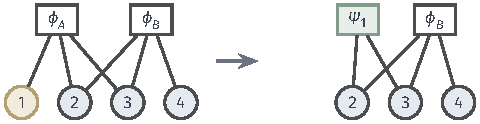
\includegraphics[width=81.284mm]{figures/03-graphs/04-local-functions-and-dynamic-programming/tikz/reading-steps/eliminate-x1.pdf}
  \caption{消去$x_1$：把读取它的$\phi_A$替换为$\psi_1(x_2,x_3)$，$\phi_B$不变。圆点为变量，方块为函数，连线表示读取关系；左侧黄色变量被汇总，右侧绿色方块是新函数。}
  \label{fig:graph-dp-elimination-trace}
\end{BookInlineFigure}

消去$x_4$：只有$\phi_B$含$4$，$S_4=\{2,3\}$。对$(x_2,x_3)$的四种取值比较$x_4=0,1$，得到
  \[
  \psi_4=\bigl(\min(2,1),\ \min(0,+\infty),\ \min(+\infty,0),\ \min(1,2)\bigr)=(1,0,0,1),
  \]
  回溯表$b_4=(1,0,1,0)$。函数集合变为$\{\psi_1,\psi_4\}$。
\begin{BookInlineFigure}
  \centering
  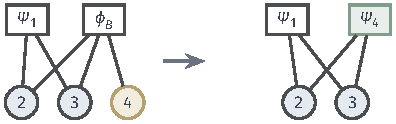
\includegraphics[width=67.035mm]{figures/03-graphs/04-local-functions-and-dynamic-programming/tikz/reading-steps/eliminate-x4.pdf}
  \caption{消去$x_4$：$\phi_B$被$\psi_4(x_2,x_3)$替换。此时两个函数只共享接口变量$x_2,x_3$。}
  \label{fig:graph-dp-elimination-trace-x4}
\end{BookInlineFigure}

消去$x_2$：$\psi_1$和$\psi_4$都含$2$，要先相加再对$x_2$取最小，$S_2=\{3\}$。$x_3=0$时两个候选为
  \[
  \psi_1(0,0)+\psi_4(0,0)=1,\qquad \psi_1(1,0)+\psi_4(1,0)=1,
  \]
  二者并列，按约定取$x_2=0$。$x_3=1$时候选为$0+0=0$与$2+1=3$，取$x_2=0$。新函数记为$\psi_2'=(1,0)$，以区别于第~\ref{sec:graph-dp-fill-in}小节先消$x_2$时的$\psi_2$；$b_2=(0,0)$。
\begin{BookInlineFigure}
  \centering
  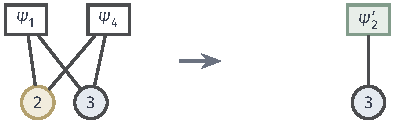
\includegraphics[width=66.784mm]{figures/03-graphs/04-local-functions-and-dynamic-programming/tikz/reading-steps/eliminate-x2.pdf}
  \caption{消去$x_2$：先把同一$(x_2,x_3)$下的$\psi_1$与$\psi_4$相加，再对$x_2$取最小。两项共同被一元函数$\psi_2'(x_3)$替换。}
  \label{fig:graph-dp-elimination-trace-x2}
\end{BookInlineFigure}

消去$x_3$：只剩$\psi_2'$，$S_3=\varnothing$，$\min(1,0)=0$在$x_3=1$处达到，$b_3=1$。函数集合只剩常数$0$，即最小成本。
\begin{BookInlineFigure}
  \centering
  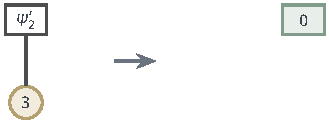
\includegraphics[width=55.785mm]{figures/03-graphs/04-local-functions-and-dynamic-programming/tikz/reading-steps/eliminate-x3.pdf}
  \caption{消去$x_3$：对最后的一元函数$\psi_2'$取最小，得到常数$0$。新函数已无变量，因而右侧没有连线。}
  \label{fig:graph-dp-elimination-trace-x3}
\end{BookInlineFigure}

最小成本有限，按逆序$3,2,4,1$回溯：
\[
\begin{gathered}
x_3=b_3=1,\qquad x_2=b_2(x_3{=}1)=0,\\
x_4=b_4(x_2{=}0,x_3{=}1)=0,\qquad x_1=b_1(x_2{=}0,x_3{=}1)=0.
\end{gathered}
\]

\begin{BookInlineFigure}
  \centering
  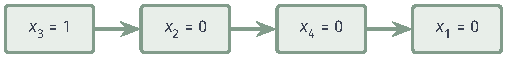
\includegraphics[width=85.785mm]{figures/03-graphs/04-local-functions-and-dynamic-programming/tikz/reading-steps/elimination-recovery.pdf}
  \caption{按消元的逆序查回溯表。先确定$x_3$，再用已知接口值依次读取$b_2,b_4,b_1$，恢复$(x_1,x_2,x_3,x_4)=(0,0,1,0)$。}
  \label{fig:graph-dp-elimination-trace-recovery}
\end{BookInlineFigure}

恢复的配置为$(0,0,1,0)$，代回表~\ref{tab:graph-dp-ternary-tables}得
\[
\phi_A(0,0,1)+\phi_B(0,1,0)=0+0=0,
\]
与枚举结果一致。

\begin{table}[!htb]
  \centering
  \small
  \begin{tabular}{@{}cccccc@{}}
    \toprule
    消去 & 取出$\mathcal F_i$ & $S_i$ & 新函数$\psi_i$ & 回溯表$b_i$ & 消元后的$\mathcal F$\\
    \midrule
    $x_1$ & $\phi_A$ & $\{2,3\}$ & $(0,0,1,2)$ & $(1,0,1,1)$ & $\{\psi_1,\phi_B\}$\\
    $x_4$ & $\phi_B$ & $\{2,3\}$ & $(1,0,0,1)$ & $(1,0,1,0)$ & $\{\psi_1,\psi_4\}$\\
    $x_2$ & $\psi_1,\psi_4$ & $\{3\}$ & $(1,0)$ & $(0,0)$ & $\{\psi_2'\}$\\
    $x_3$ & $\psi_2'$ & $\varnothing$ & $0$ & $1$ & $\{0\}$\\
    \bottomrule
  \end{tabular}
  \caption{按次序$(1,4,2,3)$对三元作用域例子消元。新函数与回溯表的取值按剩余变量的字典序列出：作用域为$\{2,3\}$时依次对应$(x_2,x_3)=(0,0),(0,1),(1,0),(1,1)$，作用域为$\{3\}$时对应$x_3=0,1$。}
  \label{tab:graph-dp-elimination-trace}
\end{table}


\paragraph{袋树上的执行过程}
同一个例子也可以直接在两个袋$B_s=\{1,2,3\}$、$B_t=\{2,3,4\}$上执行算法~\ref{alg:graph-dp-bag-dp}，取$t$为根，后序为$s,t$。本地成本为$\Phi_s=\phi_A$、$\Phi_t=\phi_B$。

$s$是叶节点，没有子消息，内部变量只有$x_1$，所以
\[
m_{s\to t}(x_2,x_3)=\min_{x_1}\phi_A(x_1,x_2,x_3).
\]
图~\ref{fig:graph-dp-bag-message-table}逐行列出了这张四项表：接口取值为$00,01,10,11$时，消息值依次为$0,0,1,2$，达到最小值的$x_1$依次为$1,0,1,1$。它与消去$x_1$得到的$\psi_1$相同。

$x_1$已经被汇总，不再出现在表中；$x_2,x_3$作为接口仍然显式保留，根袋读取这张表时要按同样的$(x_2,x_3)$取值对齐。

根处合并得$g_t=\phi_B+m_{s\to t}$，按$(x_2,x_3,x_4)$的字典序依次为
\[
g_t=(2,\,1,\,0,\,+\infty,\,+\infty,\,1,\,3,\,4),
\]
最小值$0$在$(0,1,0)$处达到。

回溯时根取$(x_2,x_3,x_4)=(0,1,0)$，查叶节点的回溯表得$b_s(0,1)=0$，即$x_1=0$。恢复的配置$(0,0,1,0)$与枚举和消元的结果相同。

\begin{figure}[!htb]
  \centering
  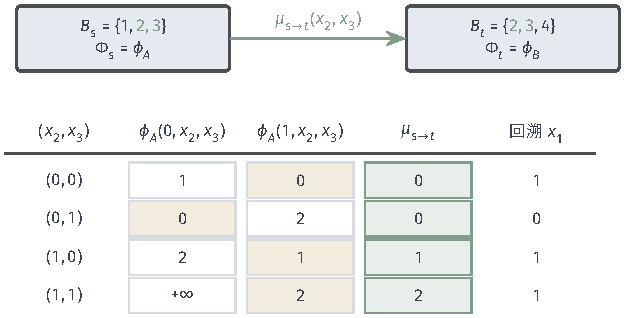
\includegraphics[width=105.650mm]{figures/01-basic-mathematics/04-graphs/tikz/c5-bag-message-table/figure.pdf}
  \caption{两袋之间的消息。左袋$B_s=\{1,2,3\}$只含$\phi_A$，右袋$B_t=\{2,3,4\}$只含$\phi_B$，接口为$\{2,3\}$（绿色）。下方表格对接口的每种取值比较$x_1=0,1$两个候选，取较小者作为消息值，黄色格是被选中的候选；绿色列是消息值，最后一列是回溯表。根袋$B_t$把消息与$\phi_B$相加后对$x_2,x_3,x_4$取最小，得到最优值$0$。}
  \label{fig:graph-dp-bag-message-table}
\end{figure}

\subsection{计算正确性}
\label{sec:graph-dp-min-cost-correctness}
\label{sec:graph-dp-bag-analysis}
\label{sec:graph-dp-elimination-analysis}

\paragraph{消息的不变量}
正确性归结为一个不变量：每条消息等于固定接口后，下方全部局部项之和的最小值。对非根节点$u$，记$D_u$为$u$及其全部后代组成的节点集合，$V_{D_u}=\bigcup_{t\in D_u}B_t$为这些袋中出现的变量，$A_{D_u}=\bigcup_{t\in D_u}A_t$为归入这些节点的局部项。

\begin{theorem}[袋消息的含义]
\label{thm:graph-dp-bag-message}
设$(\mathcal T,\{B_t\}_{t\in T})$是原始图的树分解，以$r$为根，每个局部函数恰好归入一个包含其作用域的袋。则对每个非根节点$u$和每个接口取值$\bm x_{S_u}$，
\[
m_{u\to p(u)}(\bm x_{S_u})=\min_{\bm x_{V_{D_u}\setminus S_u}}\ \sum_{a\in A_{D_u}}\phi_a(\bm x_{S_a}).
\]
进一步，$\min_{\bm x}F(\bm x)=\min_{\bm x_{B_r}}g_r(\bm x_{B_r})$。
\end{theorem}

\begin{proof}
对$|D_u|$归纳，叶节点是起点。设$u$的子节点为$c_1,\ldots,c_k$（叶节点时$k=0$）。$D_u$由$u$和各$D_{c_j}$组成，于是$A_{D_u}$分为$A_u$和各$A_{D_{c_j}}$，每个局部项恰在一处。

先看变量怎样分开。由引理~\ref{lem:graph-dp-interface-separation}应用于袋树边$\{c_j,u\}$，$V_{D_{c_j}}$与$D_{c_j}$以外各袋的公共变量都在$S_{c_j}\subseteq B_u$中。所以集合
\[
I_u,\qquad V_{D_{c_1}}\setminus B_u,\qquad\ldots,\qquad V_{D_{c_k}}\setminus B_u
\]
两两不交：$V_{D_{c_j}}\setminus B_u$中的变量不在$B_u$里，也不在其他子树中。它们的并恰为$V_{D_u}\setminus S_u$。另一方面，$A_{D_{c_j}}$中函数的变量都在$V_{D_{c_j}}$中，其中属于$B_u$的部分又在$S_{c_j}$中。

现在固定$\bm x_{B_u}$。各$A_{D_{c_j}}$中函数之和只依赖$\bm x_{S_{c_j}}$与互不相交的变量组$\bm x_{V_{D_{c_j}}\setminus B_u}$，按式~\eqref{eq:graph-dp-min-rules}后的第三条规则可以分别求最小；由归纳假设，第$j$项的最小值为$m_{c_j\to u}(\bm x_{S_{c_j}})$。归入$u$的局部项与这些变量无关，由第二条规则留在最小化之外。于是固定$\bm x_{B_u}$后的最小值是$g_u(\bm x_{B_u})$。再对$\bm x_{I_u}$求最小值，由第一条规则，就得到式~\eqref{eq:graph-dp-bag-message}。

根处的等式用同样的拆分得到：由顶点覆盖，全部变量是$B_r$与各$V_{D_c}\setminus B_r$（$c\in\operatorname{ch}(r)$）的不交并，全部局部项分为归入$r$的与归入各子树的。
\end{proof}

证明用到了三项条件：运行交集保证接口隔开两侧；顶点覆盖保证根处的汇总涉及全部变量；每个局部函数恰好归入一个容纳它的袋，保证每一项只计一次。少了任何一项，递推得到的数都可能不等于原问题的最小值。

\paragraph{任意消元次序都正确}
按消元次序直接计算时，正确性也可以用一个不变量表述，并且它对任意次序都成立。设已经按某个次序消去了下标集合$Z$中的变量，把剩余变量的一个配置记为$\bm y=\bm x_{V\setminus Z}$。消元过程保持
\begin{equation}
\sum_{f\in\mathcal F}f(\bm y)=\min_{\bm x_Z}F(\bm x_Z,\bm y)\qquad\text{对每个剩余配置}\ \bm y .
\label{eq:graph-dp-elimination-invariant}
\end{equation}

\begin{theorem}[变量消元的正确性]
\label{thm:graph-dp-elimination}
设各变量的状态集合有限，总成本由式~\eqref{eq:graph-dp-local-sum}给出。从$\mathcal F=\{\phi_a:a\in A\}$出发，按任意次序反复执行式~\eqref{eq:graph-dp-elimination-step}的消元操作，则每一步之后不变量~\eqref{eq:graph-dp-elimination-invariant}都成立。特别地，消去全部变量后剩下的常数之和等于$\min_{\bm x}F(\bm x)$；只消去$V\setminus R$中的变量时，剩余函数之和是关于$\bm x_R$的表，在每个$\bm x_R$处等于$\min_{\bm x_{V\setminus R}}F(\bm x)$。
\end{theorem}

\begin{proof}
开始时$Z=\varnothing$，当前函数之和就是$F$，不变量成立。设消去$x_i$之前不变量对$Z$成立。把当前函数分为含$i$的$\mathcal F_i$与其余部分$\mathcal F_{-i}$。固定$Z\cup\{i\}$以外的变量后，$\mathcal F_{-i}$中各函数的值与$x_i$无关，按式~\eqref{eq:graph-dp-min-rules}可以移出对$x_i$的最小化：
\[
\min_{x_i}\Bigl[\sum_{f\in\mathcal F_{-i}}f+\sum_{f\in\mathcal F_i}f\Bigr]
=\sum_{f\in\mathcal F_{-i}}f+\min_{x_i}\sum_{f\in\mathcal F_i}f
=\sum_{f\in\mathcal F_{-i}}f+\psi_i .
\]
右端正是消元后的函数之和。左端由不变量等于$\min_{x_i}\min_{\bm x_Z}F$，再由式~\eqref{eq:graph-dp-min-rules}的第一条等于$\min_{\bm x_{Z\cup\{i\}}}F$。所以不变量对$Z\cup\{i\}$成立。对消元步数归纳即得结论。
\end{proof}

这个定理说明，纯最小化中改变消元次序不改变最小值，但中间表与计算代价可以变化。三元作用域例子按次序$(2,1,3,4)$消元时，第一步得到第~\ref{sec:graph-dp-fill-in}小节的$8$项表$\psi_2$，其后依次得到$(x_3,x_4)$上的$(2,1,0,4)$、$x_4$上的$(0,1)$和常数$0$，逆序回溯同样恢复出$(0,0,1,0)$。两种次序得到相同的最小值，而最大中间表分别有$4$项和$8$项（表~\ref{tab:graph-dp-elimination-orders}）。

\paragraph{恢复的配置达到最小值}
回溯给出一致的配置：每个变量恰被赋值一次，接口变量在子节点中沿用父节点已取的值。再对$|D_u|$归纳可知，给定接口取值$\bm x^\star_{S_u}$且$m_{u\to p(u)}(\bm x^\star_{S_u})$有限时，按回溯表给$V_{D_u}\setminus S_u$赋值后，$A_{D_u}$中局部项之和恰好等于$m_{u\to p(u)}(\bm x^\star_{S_u})$。这是因为$b_u$选的内部取值达到式~\eqref{eq:graph-dp-bag-message}的最小值，使$g_u$等于消息；$g_u$中的每条子消息又由归纳假设被子树中的赋值达到，而且这些子消息有限，回溯表中有相应的记录。

在根处，所选的$\bm x^\star_{B_r}$使$g_r$等于$F^\star$，于是整个配置的成本等于$F^\star$。若$F^\star=+\infty$，任何配置都“达到”它，所以算法报告没有可行配置，而不把回溯结果当作最优解输出。逆序回溯的正确性是同一论证在消元森林上的特例；若只保存$\psi_i$而不保存回溯表，就无法直接恢复配置。

回溯表只恢复一个最优配置。若要列出全部并列最优的配置，需要在每个接口取值下记录全部最优的内部取值，而这类配置的数目本身可能随$n$指数增长。

\subsection{四环算例与边界检验}
\label{sec:graph-dp-four-cycle-min}

\paragraph{四环算例}
在四环算例的分解$\{1,2,4\}-\{2,3,4\}$上执行算法~\ref{alg:graph-dp-bag-dp}，以$\{2,3,4\}$为根。归属与第~\ref{sec:graph-dp-term-assignment}小节相同。

叶节点的接口为$\{2,4\}$，内部变量为$\{1\}$。对接口的每种取值比较$x_1=0,1$两个候选$\phi_{1,2}+\phi_{1,4}$，表~\ref{tab:graph-dp-four-cycle-min-messages}的左半部分列出了结果，消息与第~\ref{sec:graph-dp-four-cycle}小节的$\psi_1$相同。

根处合并
\[
g=\phi_{2,3}(x_2,x_3)+\phi_{3,4}(x_3,x_4)+m(x_2,x_4),
\]
表的右半部分按$(x_2,x_3,x_4)$的字典序列出。最小值$3$在$(0,0,1)$处唯一达到。

回溯时根取$(x_2,x_3,x_4)=(0,0,1)$，查叶节点的回溯表得$b(0,1)=1$，恢复$\bm x^\star=(1,0,0,1)$。这与表~\ref{tab:graph-dp-four-cycle-enumeration}的枚举结果一致；代回四项成本$1+1+1+0=3$，每项恰计一次。

\begin{table}[!htb]
  \centering
  \small
  \begin{tabular}{@{}cccc@{\qquad}cc@{}}
    \toprule
    $(x_2,x_4)$ & 候选 & $m$ & $b$ & $(x_2,x_3,x_4)$ & $g$\\
    \midrule
    $(0,0)$ & $6,\ 4$ & $4$ & $1$ & $(0,0,0)$, $(0,0,1)$ & $5$, $3$\\
    $(0,1)$ & $+\infty,\ 1$ & $1$ & $1$ & $(0,1,0)$, $(0,1,1)$ & $7$, $+\infty$\\
    $(1,0)$ & $3,\ 5$ & $3$ & $0$ & $(1,0,0)$, $(1,0,1)$ & $4$, $4$\\
    $(1,1)$ & $+\infty,\ 2$ & $2$ & $1$ & $(1,1,0)$, $(1,1,1)$ & $4$, $+\infty$\\
    \bottomrule
  \end{tabular}
  \caption{四环算例的最小成本计算。左：叶节点$\{1,2,4\}$对$x_1=0,1$的两个候选、消息值与回溯表。右：根$\{2,3,4\}$的合并值$g=\phi_{2,3}+\phi_{3,4}+m$。}
  \label{tab:graph-dp-four-cycle-min-messages}
\end{table}

改用未合并的消元森林，即按次序$(1,2,3,4)$执行算法~\ref{alg:graph-dp-variable-elimination}，第一步同样得到$\psi_1$。消去$x_2$时取出$\psi_1$与$\phi_{2,3}$，得
\[
\psi_2(x_3,x_4)=(4,2,4,3),
\]
回溯表为$(1,0,1,1)$。

消去$x_3$时取出$\psi_2$与$\phi_{3,4}$。$x_4=0$时两个候选$4+0$与$4+0$并列，按约定取$x_3=0$；$x_4=1$时候选为$2+1$与$3+\infty$。于是
\[
\psi_3(x_4)=(4,3).
\]
最后消去$x_4$得常数$3$。逆序回溯给出$x_4=1$、$x_3=0$、$x_2=0$、$x_1=1$，结果相同，中间表则与合并袋上的计算不同。

\paragraph{并列最优}
把$\phi_{2,3}(1,0)$从$1$改为$0$，其余不变。这时$(0,1,0,0)$、$(1,0,0,1)$、$(1,1,0,1)$三个配置的成本都是$3$。叶节点的消息不变，根处$g$在$(0,0,1)$、$(1,0,0)$、$(1,0,1)$三处取最小值$3$。按字典序规则，根取$(0,0,1)$，恢复的仍是$(1,0,0,1)$；若规则改为取字典序最大者，根取$(1,0,1)$，恢复$(1,1,0,1)$。两者都是最优配置，固定规则只是让输出可以复现；要得到全部最优配置，须保留全部达到值。

\paragraph{不可行}
把四项成本换成约束：$\phi_{1,2},\phi_{2,3},\phi_{3,4}$在两端相等时为$0$、不等时为$+\infty$，$\phi_{1,4}$在两端不等时为$0$、相等时为$+\infty$。每张表单独看都有可行的组合，但沿环要求$x_1=x_2=x_3=x_4$且$x_1\neq x_4$，互相矛盾。

叶节点的消息为
\[
m(x_2,x_4)=(+\infty,0,0,+\infty),
\]
即只有$x_2\neq x_4$时存在可行的$x_1$。根处$\phi_{2,3}+\phi_{3,4}$要求$x_2=x_3=x_4$，此时$m=+\infty$，所以$g$的八项全是$+\infty$，算法报告不可行，不做恢复。$+\infty$按运算约定沿消息传递，不需要特殊处理。

\paragraph{孤立变量与多个分量}
在原问题上再加两个分量：一个没有任何局部项的孤立变量$x_5\in\{0,1,2\}$，以及一条边$\{6,7\}$上的成本$\phi_{6,7}$，其表的行对应$x_6$、列对应$x_7$：
\[
\phi_{6,7}=\begin{bmatrix}2&1\\0&3\end{bmatrix}.
\]
结构上增加袋$\{5\}$和$\{6,7\}$，各用一条空接口的边连到根$\{2,3,4\}$。

袋$\{5\}$没有局部项，$g\equiv0$，对三个状态取最小得标量消息$0$，回溯记录$x_5=0$（字典序最小）。袋$\{6,7\}$的接口也为空，消息是$\min\phi_{6,7}=0$，在$(x_6,x_7)=(1,0)$处达到。

根把这两个标量加进$g$，最小成本为$3+0+0=3$，恢复的配置在原四个变量上不变，并有$x_5=0$、$(x_6,x_7)=(1,0)$。孤立变量虽不影响最小值，仍须出现在某个袋中，才会在恢复时被赋值。

% 第13章第3节：带保留变量的最小成本（条件最小成本表、查询结构与局部项归属、条件最小成本表的计算、条件最优配置的恢复、计算正确性、条件最小成本表的检验）。

\section{带保留变量的最小成本}
\label{sec:graph-dp-retained-min}

有时不需要把全部变量都优化掉，而是想知道：若把某几个变量固定成某组值，其余变量最好能做到多少。比较这几个变量的不同取值时，需要的正是这样一张表。本节指定一组暂不消去的变量，求出它们每种固定取值下的最小成本；输出是一张以这些变量的取值为索引的表。

\subsection{条件最小成本表}
\label{sec:graph-dp-conditional-table}

设保留集为$R\subseteq V$。对每个固定的$\bm x_R$，在其余变量上最小化，得到
\begin{equation}
F_R(\bm x_R)=\min_{\bm x_{V\setminus R}}F(\bm x_R,\bm x_{V\setminus R}).
\label{eq:graph-dp-conditional-table}
\end{equation}
这张表称为$R$上的\term{条件最小成本表}。它有$\prod_{i\in R}|\mathcal X_i|$个表项，保留变量是表的索引，不在这里继续取最小；表项为$+\infty$表示把$R$固定成这组值后没有可行配置。

对整张表再取最小，就回到整体最小成本：
\[
\min_{\bm x_R}F_R(\bm x_R)=F^\star,
\]
这由式~\eqref{eq:graph-dp-min-rules}的第一条得到。

表的两种极端情形是：$R=\varnothing$时表只有一项，就是$F^\star$；$R=V$时不消去任何变量，表就是$F$本身。第~\ref{sec:graph-dp-tree-two-pass}小节的各顶点最小成本表是$R$为单个变量时的特例。

\subsection{查询结构与局部项归属}
\label{sec:graph-dp-query-assignment}

计算使用第~\ref{sec:graph-dp-query-structure}小节的查询结构：在原始图中把$R$补成团，为补边后的图$\mathcal G_R$构建树分解，并选一个包含$R$的袋作根。用消元表示时，就是只消去$V\setminus R$，所有剩余作用域含于$R$的袋连到根袋$B_R=R$（算法~\ref{alg:graph-dp-order-to-decomposition}）。

局部项的归属沿用第~\ref{sec:graph-dp-term-assignment}小节：每项归入一个容纳其作用域的袋。按消元表示，含待消去变量的项归入其中最早消去的变量对应的袋，仅涉及$R$的局部项与常数项归入根袋。

补边由查询决定，是本问题结构输入的一部分。补边后的树宽可能大于原图的树宽，因此计算代价要按实际使用的结构估计，不能直接沿用无保留变量时的最优树宽。

\subsection{条件最小成本表的计算}
\label{sec:graph-dp-conditional-computation}

非根节点的计算与第~\ref{sec:graph-dp-min-cost}节完全相同：按式~\eqref{eq:graph-dp-bag-merge}合并本地成本与子消息，按式~\eqref{eq:graph-dp-bag-message}对内部变量取最小，接口变量保留在消息的索引中。由于根袋包含$R$，$R$中的变量不会是任何非根节点的内部变量（见第~\ref{sec:graph-dp-conditional-correctness}小节），它们若出现在某个非根袋中，必定在该袋的接口里，随消息向上传递。

区别只在根袋。根$r$合并得到$g_r(\bm x_{B_r})$后，只消去$B_r\setminus R$中的变量：
\begin{equation}
F_R(\bm x_R)=\min_{\bm x_{B_r\setminus R}}g_r(\bm x_{B_r}).
\label{eq:graph-dp-conditional-root}
\end{equation}
对每个保留配置$\bm x_R$留下一个最小成本，组成整张表。若$B_r=R$，根处不取最小，$F_R=g_r$。

原始图不连通时，不含$R$的分量经空接口交来标量，即各自的最小成本；它们作为常数加到表的每一项上。用消元表示时，这一计算就是定理~\ref{thm:graph-dp-elimination}的后半部分：只消去$V\setminus R$中的变量后，剩余函数之和就是$F_R$。

\subsection{条件最优配置的恢复}
\label{sec:graph-dp-conditional-recovery}

给定使$F_R(\bm x_R)$有限的保留配置，可以恢复一个条件最优配置，即在$\bm x_R$固定时达到$F_R(\bm x_R)$的配置。做法是在根处对每个$\bm x_R$另记一张回溯表$b_r(\bm x_R)$，记录达到式~\eqref{eq:graph-dp-conditional-root}最小值的$\bm x_{B_r\setminus R}$。

恢复时保持$\bm x_R$不变，从根的回溯表读出根袋中其余变量，再按前序沿袋树查各非根节点的回溯表，与第~\ref{sec:graph-dp-min-cost-recovery}小节相同。表项为$+\infty$时报告这个固定配置不可行，不做恢复；有多个条件最优解时沿用字典序最小的选取规则。

\subsection{计算正确性}
\label{sec:graph-dp-conditional-correctness}

先说明保留变量不会被提前汇总。设$v\in R$。根袋包含$R$，所以$r\in T_v$，$T_v$中离根最近的节点就是$r$；由引理~\ref{lem:graph-dp-unique-internal}，$v$只在根作内部变量。等价地说，含$v$的每个非根袋到根的路径上每个袋都含$v$，所以$v$总在这些袋的接口里。

再逐个固定$\bm x_R$。对固定的$\bm x_R$，记$F^{(\bm x_R)}(\bm x_{V\setminus R})=F(\bm x_R,\bm x_{V\setminus R})$，它仍是局部函数之和：把每个局部函数中$R$的分量代入固定值即可。非根节点的消息在这组$\bm x_R$处的取值，正是对$F^{(\bm x_R)}$执行第~\ref{sec:graph-dp-min-cost}节递推得到的消息，因为$R$中的变量从不在非根节点被取最小，只是作为索引被带着走。由定理~\ref{thm:graph-dp-bag-message}，每条消息等于固定接口后下方局部项之和的最小值；在根处对$B_r\setminus R$取最小，得到$\min F^{(\bm x_R)}=F_R(\bm x_R)$。

条件最优配置的正确性同样沿用第~\ref{sec:graph-dp-min-cost-correctness}小节的论证，只是根处的最小点在$\bm x_R$固定的条件下选取；表项为$+\infty$时对应没有可行解。由定理~\ref{thm:graph-dp-elimination}，仅改变$V\setminus R$中变量的消去次序时，各表项不变，改变的只是中间表和代价。

\subsection{条件最小成本表的检验}
\label{sec:graph-dp-retained-check}

\paragraph{四环上的查询}
在四环算例上取$R=\{1,3\}$。第~\ref{sec:graph-dp-four-cycle-construction}小节已在补边$\{1,3\}$后的图上按次序$(2,4)$构建了查询结构：两个袋$\{1,2,3\}$与$\{1,3,4\}$都连到根袋$\{1,3\}$，接口都是$\{1,3\}$，内部变量分别是$x_2$与$x_4$。按消元规则，$\phi_{1,2},\phi_{2,3}$归入$\{1,2,3\}$，$\phi_{3,4},\phi_{1,4}$归入$\{1,3,4\}$，根袋没有本地成本。

图~\ref{fig:graph-dp-retained-query}展示这个查询专用的结构：$x_2$和$x_4$在两个子袋中分别消去，$x_1,x_3$一直保留到根袋，成为输出表的两个索引。

\begin{figure}[!htb]
  \centering
  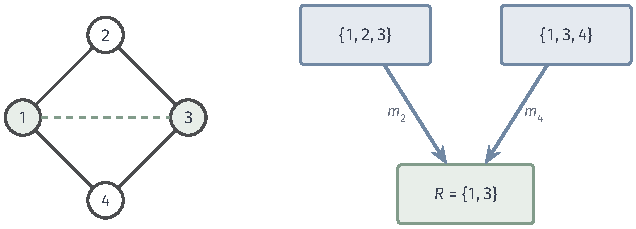
\includegraphics[width=107.500mm]{figures/03-graphs/04-local-functions-and-dynamic-programming/tikz/dp-retained-query/figure.pdf}
  \caption{四环上保留$R=\{1,3\}$的查询结构。左图的绿色虚线是为使保留集成团而补入的结构边，不增加局部成本；右图的两个子袋分别消去$x_2,x_4$，消息在根袋按同一组$(x_1,x_3)$相加。根袋恰为$R$，因此不再取最小。}
  \label{fig:graph-dp-retained-query}
\end{figure}

两个子节点的消息为
\[
\begin{aligned}
m_2(x_1,x_3)&=\min_{x_2}\bigl[\phi_{1,2}(x_1,x_2)+\phi_{2,3}(x_2,x_3)\bigr],\\
m_4(x_1,x_3)&=\min_{x_4}\bigl[\phi_{3,4}(x_3,x_4)+\phi_{1,4}(x_1,x_4)\bigr].
\end{aligned}
\]
根袋就是$R$，不再取最小，$F_R=m_2+m_4$。表~\ref{tab:graph-dp-four-cycle-retained}列出了各候选、回溯表与结果。

\begin{table}[!htb]
  \centering
  \small
  \begin{tabular}{@{}cccccccc@{}}
    \toprule
    $(x_1,x_3)$ & $m_2$的候选 & $m_2$ & $b_2$ & $m_4$的候选 & $m_4$ & $b_4$ & $F_R$及条件最优配置\\
    \midrule
    $(0,0)$ & $4,\ 1$ & $1$ & $1$ & $3,\ +\infty$ & $3$ & $0$ & $4$，$(0,1,0,0)$\\
    $(0,1)$ & $6,\ 1$ & $1$ & $1$ & $3,\ +\infty$ & $3$ & $0$ & $4$，$(0,1,1,0)$\\
    $(1,0)$ & $2,\ 3$ & $2$ & $0$ & $3,\ 1$ & $1$ & $1$ & $3$，$(1,0,0,1)$\\
    $(1,1)$ & $4,\ 3$ & $3$ & $1$ & $3,\ +\infty$ & $3$ & $0$ & $6$，$(1,1,1,0)$\\
    \bottomrule
  \end{tabular}
  \caption{四环算例在$R=\{1,3\}$上的条件最小成本表。“候选”依次对应内部变量取$0,1$；$b_2$、$b_4$是达到最小值的$x_2$、$x_4$；最后一列是由回溯表恢复的条件最优配置。}
  \label{tab:graph-dp-four-cycle-retained}
\end{table}

逐项用表~\ref{tab:graph-dp-four-cycle-enumeration}核对：
\begin{itemize}
  \item $x_1=0,x_3=0$的四个配置成本为$7,+\infty,4,+\infty$，最小$4$在$(0,1,0,0)$；
  \item $x_1=0,x_3=1$的四个为$9,+\infty,4,+\infty$，最小$4$在$(0,1,1,0)$；
  \item $x_1=1,x_3=0$的四个为$5,3,6,4$，最小$3$在$(1,0,0,1)$；
  \item $x_1=1,x_3=1$的四个为$7,+\infty,6,+\infty$，最小$6$在$(1,1,1,0)$。
\end{itemize}
四个表项及条件最优配置都与表中一致。

对整张表取最小，得到
\[
\min(4,4,3,6)=3,
\]
在$(x_1,x_3)=(1,0)$处达到，相应的条件最优配置$(1,0,0,1)$就是第~\ref{sec:graph-dp-four-cycle-min}小节的整体最优配置，两种计算互相印证。

这个查询不能直接用分解$\{1,2,4\}-\{2,3,4\}$回答：那里没有袋同时含$x_1$和$x_3$，$x_1$会在叶节点被取最小。

\paragraph{两个边界}
$R=\varnothing$时不保留变量，查询结构就是原来的结构，表只有一项，计算退化为第~\ref{sec:graph-dp-min-cost}节，四环上为$F^\star=3$。$R=V$时不消去任何变量：补边后的图是完全图，根袋包含全部变量，$F_R=g_r$就是把全部局部项相加的$16$项表，即表~\ref{tab:graph-dp-four-cycle-enumeration}本身。前者不保留任何变量，后者不消去任何变量，一般的查询介于二者之间，输出表的大小与根袋的宽度也随之介于二者之间。

% 第13章第4节：计数和求和（可行配置计数、求和、无保留变量时的汇总、保留变量的累计表、计算正确性、求和与取最小的顺序、四环算例与结果检验）。

\section{计数和求和}
\label{sec:graph-dp-semiring}
\label{sec:graph-dp-counting-sums}

最小成本只关心最好的一个配置。另一类问题要对全部配置汇总：可行配置有多少个，或者按局部权重之积给每个配置一个权重，全部权重加起来是多少。本节先用约束指示函数计算可行配置数，再把指示值推广为非负有限权重。两种计算都把“局部项相加、对变量取最小”换成“局部值相乘、对变量求和”，结构、归属和处理次序都不变；变化在于数值的组合与汇总方式，以及输出的含义。

\subsection{可行配置计数}
\label{sec:graph-dp-feasible-count}

把每个局部函数换成它的可行性指示
\[
\iota_a(\bm x_{S_a})=\begin{cases}1,&\phi_a(\bm x_{S_a})<+\infty,\\0,&\phi_a(\bm x_{S_a})=+\infty.\end{cases}
\]
一个配置可行，当且仅当这些指示全为$1$，即它们的乘积为$1$。于是可行配置数为
\begin{equation}
N=\sum_{\bm x\in\mathcal X}\ \prod_{a\in A}\iota_a(\bm x_{S_a}).
\label{eq:graph-dp-feasible-count}
\end{equation}
输入与最小成本问题相同（只用到哪些组合被禁止），输出是一个非负整数。

在袋树上计算时，节点$u$先把归入它的指示值与子节点交来的计数相乘，
\begin{equation}
h_u(\bm x_{B_u})=\prod_{a\in A_u}\iota_a(\bm x_{S_a})\cdot\prod_{c\in\operatorname{ch}(u)}n_{c\to u}(\bm x_{S_c}),
\label{eq:graph-dp-count-merge}
\end{equation}
再对接口外的状态求和，得到发往父节点的计数消息
\begin{equation}
n_{u\to p(u)}(\bm x_{S_u})=\sum_{\bm x_{I_u}}h_u(\bm x_{S_u},\bm x_{I_u}).
\label{eq:graph-dp-count-message}
\end{equation}
它的含义是：接口取这组值时，$u$下方的变量有多少种取值能使下方全部约束满足。

两种空运算的约定与最小成本不同：空乘积取$1$，求和从$0$开始。没有局部项归入、也没有子节点的袋，$h_u\equiv1$，但求和仍要累计内部变量的全部状态。孤立变量$x_v$单独成袋$\{v\}$时，消息是$\sum_{x_v}1=|\mathcal X_v|$，不能直接把它的计数设为$1$：它不受约束，每个状态都与其余变量的每个可行取值组合成不同的可行配置。

\subsection{求和}
\label{sec:graph-dp-weighted-sum}

把指示值推广为非负有限的局部权重$w_a(\bm x_{S_a})\geq0$，配置的权重定义为各局部权重之积
\[
W(\bm x)=\prod_{a\in A}w_a(\bm x_{S_a}),
\]
要求的是全部配置的权重总和
\begin{equation}
Z=\sum_{\bm x\in\mathcal X}\ \prod_{a\in A}w_a(\bm x_{S_a}).
\label{eq:graph-dp-weighted-sum}
\end{equation}
可行配置计数是取$w_a=\iota_a$的特例。

袋树上的计算与计数相同，只是把指示值换成权重。把本袋权重与子消息的乘积记为
\[
h_u(\bm x_{B_u})=\prod_{a\in A_u}w_a(\bm x_{S_a})\cdot\prod_{c\in\operatorname{ch}(u)}z_{c\to u}(\bm x_{S_c}),
\]
再对接口外状态求和，得到消息
\begin{equation}
z_{u\to p(u)}(\bm x_{S_u})=\sum_{\bm x_{I_u}}h_u(\bm x_{B_u});
\label{eq:graph-dp-sum-message}
\end{equation}
若没有接口外变量，就直接把这个乘积作为消息。

消息表照样以接口为索引，但不再需要回溯表：计数和加权总和是对全部配置的汇总，没有“达到它的配置”。

链上这一递推就是矩阵乘法。把$z_{k-1\to k}$看作行向量，把成对权重看作矩阵，矩阵的元素是$w_{k-1,k}(x_{k-1},x_k)$。于是求和
\[
\sum_{x_{k-1}}z_{k-1\to k}(x_{k-1})\,w_{k-1,k}(x_{k-1},x_k)
\]
正是行向量右乘矩阵。一般袋上对多个变量相乘再求和，则是沿指定轴汇总的张量运算。这些运算可参考\BookChapterRef{chap:linear-operations}{卷二“向量、矩阵与张量的运算”章}。

\subsection{无保留变量时的计数与求和汇总}
\label{sec:graph-dp-total-aggregation}

不保留变量时，根$r$合并得到$h_r$，再对根袋的全部状态求和：
\begin{equation}
Z=\sum_{\bm x_{B_r}}h_r(\bm x_{B_r}),
\label{eq:graph-dp-root-sum}
\end{equation}
输出一个总计数或加权总和。根袋没有变量时（例如只用来连接各分量的空袋），直接取它的合并值。

原始图不连通时，各分量的根经空接口交来标量，即各分量的总计数或总和；空接口意味着结果是单表项标量，但发出它的节点仍须对自己袋中的状态求和。这些标量作为因子乘进根的合并值，所以非连通分量的结果相乘。这与有限集合的乘法原理一致：各分量的取值互相独立地组合。

\paragraph{三元作用域例子}
表~\ref{tab:graph-dp-weights}给出三元作用域例子的权重表，权重恰在禁止的组合处为$0$。在分解$\{1,2,3\}-\{2,3,4\}$上，表~\ref{tab:graph-dp-three-aggregations}对接口的每种取值并列三种任务的左袋消息和右袋汇总值，最后一行是根处的结果：最小成本为$0$，可行配置有$10$个，权重总和为$19$。逐一枚举$16$个配置可以核对这三个数，其中最小成本和可行配置数已在第~\ref{sec:graph-dp-problem}小节的枚举中得到。

\begin{table}[!htb]
  \centering
  \caption{三元作用域例子的非负局部权重。第一列的三位二进制串对$w_A$表示$(x_1,x_2,x_3)$，对$w_B$表示$(x_2,x_3,x_4)$；权重为$0$的位置恰是表~\ref{tab:graph-dp-ternary-tables}中成本为$+\infty$的位置。}
  \label{tab:graph-dp-weights}
  \begin{tabular}{ccccccccc}
    \toprule
    取值 & $000$ & $001$ & $010$ & $011$ & $100$ & $101$ & $110$ & $111$\\
    \midrule
    $w_A$ & $1$ & $2$ & $1$ & $0$ & $2$ & $1$ & $1$ & $1$\\
    $w_B$ & $1$ & $1$ & $2$ & $0$ & $0$ & $2$ & $1$ & $2$\\
    \bottomrule
  \end{tabular}
\end{table}

\begin{table}[!htb]
  \centering
  \caption{三种任务在同一接口上的消息。最小成本使用$\min$与$+$，可行计数与加权总和使用$\sum$与$\times$。“左”列是从$\{1,2,3\}$发出的消息，对$x_1$汇总；“右”列是根袋$\{2,3,4\}$对$x_4$的汇总；根处对每个接口取值组合两列（最小成本相加，其余相乘），再对接口汇总（最小成本取最小，其余求和）。}
  \label{tab:graph-dp-three-aggregations}
  \begin{tabular}{ccccccc}
    \toprule
    & \multicolumn{2}{c}{最小成本} & \multicolumn{2}{c}{可行计数} & \multicolumn{2}{c}{加权总和}\\
    \cmidrule(lr){2-3}\cmidrule(lr){4-5}\cmidrule(lr){6-7}
    $(x_2,x_3)$ & 左 & 右 & 左 & 右 & 左 & 右\\
    \midrule
    $(0,0)$ & $0$ & $1$ & $2$ & $2$ & $3$ & $2$\\
    $(0,1)$ & $0$ & $0$ & $2$ & $1$ & $3$ & $2$\\
    $(1,0)$ & $1$ & $0$ & $2$ & $1$ & $2$ & $2$\\
    $(1,1)$ & $2$ & $1$ & $1$ & $2$ & $1$ & $3$\\
    \midrule
    根处 & \multicolumn{2}{c}{$\min(1,0,1,3)=0$} & \multicolumn{2}{c}{$4+2+2+2=10$} & \multicolumn{2}{c}{$6+6+4+3=19$}\\
    \bottomrule
  \end{tabular}
\end{table}

以接口取$(1,1)$的一行为例：$x_1=0$的一行被禁止，左袋的最小成本消息为$\min(+\infty,2)=2$，计数消息为$0+1=1$，加权消息为$0+1=1$。三种任务的计算量与表大小相同，但输出含义不同：最小成本是一个配置的值，可以回溯出达到它的配置；计数和加权总和是对全部配置的汇总。

\subsection{保留变量的累计表}
\label{sec:graph-dp-retained-aggregation}

给定保留集$R$，使用根袋覆盖$R$的查询结构（第~\ref{sec:graph-dp-query-assignment}小节），非根节点照常计算，根处只对$B_r\setminus R$求和：
\begin{equation}
Z_R(\bm x_R)=\sum_{\bm x_{B_r\setminus R}}h_r(\bm x_{B_r}).
\label{eq:graph-dp-retained-sum}
\end{equation}
结果以$\bm x_R$为索引，逐项表示把$R$固定成这组值时的可行配置数（指示权重）或权重总和。再对所有$\bm x_R$求和，才得到第~\ref{sec:graph-dp-total-aggregation}小节的总量$Z$。

与条件最小成本表相比，累计表的每一项不是一个配置的值，而是一组配置的累计；它也不需要回溯表。不含$R$的分量交来的标量作为因子乘到表的每一项上。

\subsection{计算正确性}
\label{sec:graph-dp-sum-correctness}

\paragraph{求和的三条规则}
最小成本递推所用的三条最小值规则，在求和与相乘下有完全对应的形式。设$y,z$在有限集合中取值，$h,g$取非负有限值，$c$与$y$无关，则
\[
\sum_{y,z}h(y,z)=\sum_z\sum_y h(y,z),\qquad \sum_y c\,g(y)=c\sum_y g(y),
\]
并且对取值于互不相交变量组$y_1,\ldots,y_k$的函数，
\[
\sum_{y_1,\ldots,y_k}\prod_j g_j(y_j)=\prod_j\sum_{y_j}g_j(y_j).
\]
第一条是有限求和的重排；第二条是乘法对加法的分配律；第三条由分配律展开乘积得到，展开后的每一项恰对应各$y_j$的一组取值。

\paragraph{消息的含义}
仿照定理~\ref{thm:graph-dp-bag-message}，记号同前，求和任务的消息满足
\[
z_{u\to p(u)}(\bm x_{S_u})=\sum_{\bm x_{V_{D_u}\setminus S_u}}\ \prod_{a\in A_{D_u}}w_a(\bm x_{S_a}),
\]
并且$Z=\sum_{\bm x_{B_r}}h_r(\bm x_{B_r})$。证明逐字沿用那里的拆分：变量集合$I_u$与各$V_{D_{c_j}}\setminus B_u$两两不交，并恰好组成$V_{D_u}\setminus S_u$；固定$\bm x_{B_u}$后，各子树的乘积只依赖互不相交的变量组，由第三条规则分别求和，由归纳假设得到各子消息；归入$u$的权重由第二条规则提到求和号外；最后由第一条规则对$\bm x_{I_u}$求和。

这一论证同时说明每个配置恰被累计一次。下方变量的每一组取值，唯一地分解为内部变量的一组取值和各子树中变量的一组取值；分配律展开后，每组取值恰好贡献一个乘积项$\prod_{a\in A_{D_u}}w_a$。取指示权重时，这个乘积是$1$或$0$，消息就是可行取值的个数，根处给出可行配置数。

逐项固定保留变量，同样的论证给出累计表~\eqref{eq:graph-dp-retained-sum}的正确性，全表求和得到总量。固定输入、保留集和输出要求后，仅改变待求和变量的消去次序不改变结果，因为有限求和可以任意重排；定理~\ref{thm:graph-dp-elimination-equals-messages}的对应关系也照样成立。

\paragraph{共同的代数结构}
三种任务共用同一套递推，是因为它们的运算满足同样的代数规则。每种任务都用到两种运算，分工不同：一种把同一配置的各局部项组合成这个配置的值（相加或相乘），另一种把不同取值的结果汇总成一个数（取最小或全部加起来）。消息之所以能在局部提前汇总，靠的是“先组合再汇总”与“先汇总再组合”结果相同，例如$a+\min(b,c)=\min(a+b,a+c)$、$a(b+c)=ab+ac$：与被汇总变量无关的项$a$可以留到汇总之后再组合。

把这些规则抽象出来。设集合$\mathcal S$上有两种运算：$\oplus$用于跨不同取值的汇总，$\otimes$用于在一个配置内组合各局部项。若两种运算都满足结合律和交换律，各有单位元$\bar0$与$\bar1$，满足$\bar0\otimes a=\bar0$，并且$\otimes$对$\oplus$满足分配律
\[
a\otimes(b\oplus c)=(a\otimes b)\oplus(a\otimes c),
\]
就称$(\mathcal S,\allowbreak\oplus,\allowbreak\otimes,\allowbreak\bar0,\allowbreak\bar1)$为交换\term{半环}（semiring）。

最小成本对应$(\mathbb R\cup\{+\infty\},\allowbreak\min,\allowbreak+,\allowbreak+\infty,\allowbreak0)$，此时分配律就是$a+\min(b,c)=\min(a+b,a+c)$；计数对应自然数上的$(+,\times,0,1)$；加权求和对应非负实数上的$(+,\times,0,1)$；只判断是否存在可行配置时，还可以用布尔值上的“或”与“且”。

把变量消元和袋消息中的$\min$换成$\oplus$、$+$换成$\otimes$，前面的正确性证明逐字成立，因为证明只用到了结合律、交换律和分配律。半环不要求减法或除法。

\subsection{求和与取最小的顺序}
\label{sec:graph-dp-mixed-order}

上面的换序结论只针对同一种汇总：纯最小化中可以任意交换取最小的次序，纯求和中可以任意交换求和的次序。把本节的求和与第~\ref{sec:graph-dp-min-cost}节的取最小放在一起，情况就不同了。

取一张两行两列的成本表$h(y,z)$，两行分别为$(0,1)$与$(1,0)$，即$h(0,0)=h(1,1)=0$、$h(0,1)=h(1,0)=1$。每行先对$z$求和得$1$与$1$，再对两行取最小，得到
\[
\min_y\sum_z h(y,z)=\min(1,1)=1 .
\]
反过来先对每一列在两行之间取最小，两列都得到$0$，再求和，得到
\[
\sum_z\min_y h(y,z)=0+0=0 .
\]
前者要求所有$z$共用同一个$y$，后者允许$y$随$z$改变，所以两种顺序回答的是不同的问题。

\paragraph{混合汇总}
不同变量混合使用求和与取最小（或取最大）时，须按所求结果确定运算顺序，不能直接沿用纯求和或纯最小化的换序结论。例如对表$h(x,y)$，$h(0,0)=h(1,1)=4$、$h(0,1)=h(1,0)=0$，有
\[
\max_x\sum_y h(x,y)=4,\qquad \sum_y\max_x h(x,y)=8 .
\]
这类混合问题只能按限定的次序消元：被外层汇总的变量必须最后处理，消元次序因而受到约束，所需的中间表可能比单一汇总时大。把非负权重归一化为概率还要求总和为正且有限；这些概率解释、边缘化查询以及带环图上的近似消息方法，都留到后续的概率推断内容。

\subsection{四环算例与结果检验}
\label{sec:graph-dp-four-cycle-sums}

\paragraph{约束指示表与权重表}
四环算例的约束指示表由表~\ref{tab:graph-dp-four-cycle-costs}读出：只有$\iota_{3,4}(1,1)=0$与$\iota_{1,4}(0,1)=0$，其余指示值都是$1$。另取一组非负权重，在被禁止的组合处为$0$，其余取$1$或$2$，见表~\ref{tab:graph-dp-four-cycle-weights}；这些权重是教学示例，与成本表的具体数值无关。

\begin{table}[!htb]
  \centering
  \caption{四环算例的非负局部权重。行列约定与表~\ref{tab:graph-dp-four-cycle-costs}相同；权重为$0$的位置恰是成本为$+\infty$的位置。}
  \label{tab:graph-dp-four-cycle-weights}
  \begin{tabular}{cccc}
    \toprule
    $w_{1,2}(x_1,x_2)$ & $w_{2,3}(x_2,x_3)$ & $w_{3,4}(x_3,x_4)$ & $w_{1,4}(x_1,x_4)$\\
    \midrule
    $\begin{bmatrix}1&2\\2&1\end{bmatrix}$ &
    $\begin{bmatrix}2&1\\1&1\end{bmatrix}$ &
    $\begin{bmatrix}1&2\\1&0\end{bmatrix}$ &
    $\begin{bmatrix}1&0\\1&2\end{bmatrix}$\\
    \bottomrule
  \end{tabular}
\end{table}

\paragraph{总量}
在分解$\{1,2,4\}-\{2,3,4\}$上以$\{2,3,4\}$为根。叶节点对$x_1$求和：计数消息为
\[
n(x_2,x_4)=\sum_{x_1}\iota_{1,2}\,\iota_{1,4}=(2,\ 1,\ 2,\ 1),
\]
加权消息为
\[
\begin{aligned}
z(x_2,x_4)&=\sum_{x_1}w_{1,2}\,w_{1,4}\\
&=(1\cdot1+2\cdot1,\ 1\cdot0+2\cdot2,\ 2\cdot1+1\cdot1,\ 2\cdot0+1\cdot2)\\
&=(3,4,3,2),
\end{aligned}
\]
取值按$(x_2,x_4)$的字典序排列。

根处把消息与$\phi_{2,3},\phi_{3,4}$对应的指示值或权重相乘，按$(x_2,x_3,x_4)$的字典序，计数的合并值为
\[
(2,1,2,0,2,1,2,0),
\]
求和得$N=10$。加权的合并值为
\[
(6,16,3,0,3,4,3,0),
\]
求和得$Z=35$。

用表~\ref{tab:graph-dp-four-cycle-enumeration}核对：可行配置恰有$10$个。逐个计算可行配置的权重，按字典序依次为$2,1,2,2,4,16,2,1,4,1$，总和为$35$。例如最优配置$(1,0,0,1)$的权重为
\[
w_{1,2}(1,0)\,w_{2,3}(0,0)\,w_{3,4}(0,1)\,w_{1,4}(1,1)=2\cdot2\cdot2\cdot2=16.
\]

\paragraph{保留变量的累计表}
在$R=\{1,3\}$的查询结构上，两个子节点分别对$x_2$与$x_4$求和，根袋$\{1,3\}$把两条消息相乘，不再求和。按$(x_1,x_3)$的字典序，计数消息为$(2,2,2,2)$与$(1,1,2,1)$，累计表为
\[
N_R=(2,\ 2,\ 4,\ 2);
\]
加权消息为$(4,3,5,3)$与$(1,1,5,1)$，累计表为
\[
Z_R=(4,\ 3,\ 25,\ 3).
\]
全表求和分别为
\[
2+2+4+2=10=N,\qquad 4+3+25+3=35=Z.
\]

下面逐项核对。例如$x_1=1,x_3=0$时，可行配置为
\[
 (1,0,0,0),\qquad (1,0,0,1),\qquad (1,1,0,0),\qquad (1,1,0,1),
\]
共$4$个，权重之和为$4+16+1+4=25$。

\paragraph{结果的解释与边界}
计数为零表示没有可行配置：第~\ref{sec:graph-dp-four-cycle-min}小节的不可行约束变体中，叶节点的计数消息为$(0,1,1,0)$，根处要求$x_2=x_3=x_4$时这条消息为$0$，于是$N=0$，与最小成本为$+\infty$一致。

一般的加权和为零却不直接表示不可行：权重可以在可行的组合上取$0$，例如把$w_{1,2}$全部改为$0$，则$Z=0$，而可行配置仍有$10$个。

第~\ref{sec:graph-dp-four-cycle-min}小节加入孤立变量$x_5\in\{0,1,2\}$和边$\{6,7\}$后，两个新分量经空接口交来标量。袋$\{5\}$没有局部项，$h\equiv1$，计数消息为$3$。若$\phi_{6,7}$的四项都有限，袋$\{6,7\}$的计数消息为$4$；若再给它权重表
\[
w_{6,7}=\begin{bmatrix}1&1\\2&1\end{bmatrix},
\]
加权消息为$5$。根把这些标量乘进合并值，得
\[
N=10\cdot3\cdot4=120,\qquad Z=35\cdot3\cdot5=525.
\]若错把孤立变量的计数设为$1$，结果会少乘一个因子$3$。

% 第13章第5节：计算代价（状态表的规模、时间代价、存储代价、时间与存储的取舍）。

\section{计算代价}
\label{sec:graph-dp-computation-cost}

前几节的计算都给出精确结果，但所需的时间和存储可能很大。本节把已构建的袋和接口换算成实际的状态组合数，分别分析求值的时间、存储及二者的取舍。结构的构造方法见第~\ref{sec:graph-tree-decomposition-construction}节；这里给出的资源指标可以用来比较不同的构造结果，构造与核验本身的成本也一并计入任务的总成本。

\subsection{状态表的规模}
\label{sec:graph-dp-table-size}

先固定规模变量：变量个数$n$，局部项个数$|A|$，袋树节点数$N$，第$i$个变量的状态数$|\mathcal X_i|$，以及$q=\max_i|\mathcal X_i|$。对一组变量$U$，记它上面的配置数为
\[
|\mathcal X_U|=\prod_{i\in U}|\mathcal X_i| .
\]
计算中出现三类表：袋$u$上的合并表有$|\mathcal X_{B_u}|$项，接口消息和回溯表各有$|\mathcal X_{S_u}|$项（回溯表的每一项存$|I_u|$个变量的取值），保留变量的输出表有$|\mathcal X_R|$项。

在每个变量至多$q$个状态、分解宽度为$w$时，每个袋至多$w+1$个变量，袋表至多$q^{w+1}$项。但这只是上界：接口与输出仍按实际变量计算，状态数不同的变量对乘积的贡献也不同。比较两个候选结构时，应固定同一任务（同一保留集、同一输出要求），并使用实际的乘积，而不是只比较宽度。例如两个结构宽度都是$2$，一个的最大袋由三个二值变量组成（$8$项），另一个含一个十状态变量（至少$40$项），实际规模相差数倍。

图~\ref{fig:graph-dp-table-size}把这个差别落实为表项：两侧都只有三个变量，但十状态变量需要十组而不是两组配置。同为宽度$2$，并不意味着同样的读表和存储代价。

\begin{figure}[!htb]
  \centering
  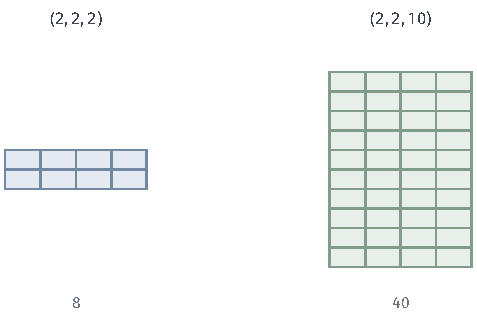
\includegraphics[width=80.617mm]{figures/03-graphs/04-local-functions-and-dynamic-programming/tikz/dp-table-size/figure.pdf}
  \caption{相同袋宽度下的实际表规模。括号给出三个变量各自的状态数，每格对应一种联合取值。左表为$2\times2\times2=8$项，右表为$2\times2\times10=40$项；四列枚举前两个二值变量，行枚举第三个变量。}
  \label{fig:graph-dp-table-size}
\end{figure}

宽度出现在指数上，这是精确计算的主要限制。$q=10$、$w=10$时一张袋表就有$10^{11}$项；若查询要求保留很多变量的联合表，输出本身也可能大得不可承受，这时任何精确方法都必须至少写出整张表。

四环算例中，分解$\{1,2,4\}-\{2,3,4\}$的两个袋各有$8$项，接口消息和回溯表各有$4$项；$R=\{1,3\}$的查询结构有两个$8$项的袋、一个$4$项的根袋，输出表$4$项。按次序$(1,2,3,4)$不合并时，四个消元簇的配置数为$8,8,4,2$。

\subsection{时间代价}
\label{sec:graph-dp-time-cost}

约定表查询、加法、乘法和比较各计一次基本运算。处理节点$u$时，要对$\bm x_{B_u}$的每种取值读取归入$u$的每个局部项一次、读取每条子消息一次，把它们组合起来，再参与一次取最小或求和，所以工作量约为
\[
|\mathcal X_{B_u}|\,\bigl(|A_u|+|\operatorname{ch}(u)|+1\bigr).
\]
对全部节点求和，利用袋树中$\sum_u|\operatorname{ch}(u)|=N-1$，求值时间为
\[
\sum_{u}|\mathcal X_{B_u}|\,\bigl(|A_u|+|\operatorname{ch}(u)|+1\bigr)=O\bigl((|A|+N)\,q^{w+1}\bigr).
\]
可见单个袋表的上界$q^{w+1}$还要乘以袋数和每项的工作量，才给出总时间。

按消元次序计算时，消去$x_i$要对$\{i\}\cup S_i$的至多$q^{|S_i|+1}$种取值各读取$\mathcal F_i$中每个函数一次，时间约为
\[
|\mathcal F_i|\,q^{|S_i|+1}.
\]
每个函数恰好在它的某个变量被消去时被取出一次，原有函数$|A|$个，新函数至多$n$个，所以各步的$|\mathcal F_i|$之和不超过$|A|+n$；按变量维护索引的开销也与函数个数成正比。若诱导宽度为$w$，总时间为
\[
O\bigl((|A|+n)\,q^{w+1}\bigr),
\]
而枚举为$|A|\,q^n$。

除向上的求值外，还要计入结果输出与配置恢复。条件最小成本表或累计表的输出要写出$|\mathcal X_R|$项。恢复一个配置时每个节点只查一次回溯表，共$O\bigl(\sum_u|B_u|\bigr)$次读写，与求值相比可以忽略。若还需要每个袋上各取值的最小总成本，就像第~\ref{sec:graph-dp-tree-two-pass}小节那样再按前序发送一遍反向消息，时间约加倍。

结构构造与核验的时间单独计算，再加入任务的总时间：模拟消元为$O\bigl(n+m+\sum_t d_t^2\bigr)$（第~\ref{sec:graph-dp-clusters-to-decomposition}小节），检验为袋大小的多项式（第~\ref{sec:graph-dp-construction-check}小节）。同一结构用于多组数值时，这部分只付一次。

计数中的整数加乘在上面各计一次基本运算。若要考虑位复杂度，还须按数值的位数分析：可行配置数至多为$\prod_i|\mathcal X_i|\leq q^n$，需要约$n\log_2q$位，大规模问题中一次加乘的实际代价随位数增长；加权求和若用浮点数，还要另行分析舍入误差。

\subsection{存储代价}
\label{sec:graph-dp-memory-cost}

存储要分清对象，并按计算过程中同时保留的对象计算峰值，不能把累计生成的表项总量或单个接口的规模直接当作峰值。计算中要存放的对象有四类：
\begin{itemize}
  \item 接口消息：每张$|\mathcal X_{S_u}|$项，从生成起保留到父节点用完为止；
  \item 临时袋表：处理节点$u$时的合并表，若整张存放有$|\mathcal X_{B_u}|$项；
  \item 达到值记录：每个非根节点一张回溯表，$|\mathcal X_{S_u}|$项，每项存$|I_u|$个取值，要保留到恢复结束；
  \item 输出表：保留变量查询的$|\mathcal X_R|$项。
\end{itemize}

临时袋表不必整张存放。对接口的每个取值，可以逐个枚举内部变量的取值，现场计算$g_u$的一项并立即并入当前的最小值（或累加和），算完一个接口取值就写出消息的一项。这样处理节点$u$时只需$O(|B_u|)$的工作空间，而不是$|\mathcal X_{B_u}|$；代价是对局部项和子消息的读取顺序不再连续，常数因子可能变大。

消息的保留时间取决于后序。只求最优值而不恢复配置时，子节点的消息在父节点处理完后即可释放，所以任一时刻保留的只是“已处理完、父节点尚未处理”的那些节点的消息。链状袋树上同时只有一条消息；一个根下挂很多叶节点时，处理根之前全部叶节点的消息同时存在。峰值是这些同时存在的消息之和，加上当前节点的工作空间，而不是全部消息的总和。

图~\ref{fig:graph-dp-message-frontier}对比了两种后序计算的中间时刻。只需最优值、并在父节点使用后释放子消息时，链上只留下最近生成的一条消息；星形结构在处理根之前则须同时保存各叶节点的消息。

\begin{figure}[!htb]
  \centering
  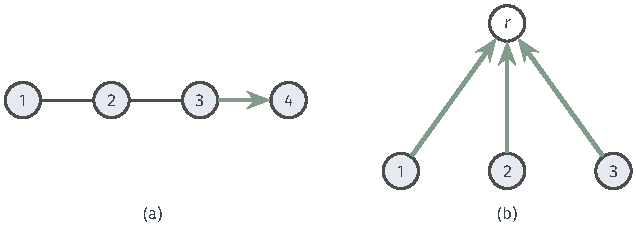
\includegraphics[width=107.500mm]{figures/03-graphs/04-local-functions-and-dynamic-programming/tikz/dp-message-frontier/figure.pdf}
  \caption{同时存活的消息决定峰值存储。圆点表示袋，绿色箭头表示已经生成、仍待父袋读取的消息。(a)链上袋$1,2$的消息已被后继使用并释放，仅袋$3$的消息仍在；(b)根$r$尚未处理，三个叶袋的消息同时存在。此处比较消息存储，不包含回溯表或输出表。}
  \label{fig:graph-dp-message-frontier}
\end{figure}

需要恢复配置时，回溯表要保留到前序回溯走完，存储为$\sum_u|\mathcal X_{S_u}|\cdot|I_u|$量级，这时可以释放的只有消息。

四环算例中，最小成本计算的峰值是一条$4$项消息加根处的工作空间；恢复配置还要保留一张$4$项的回溯表。$R=\{1,3\}$的查询中，处理根之前两条$4$项消息同时存在，输出表另有$4$项。

\subsection{时间与存储的取舍}
\label{sec:graph-dp-time-memory-tradeoff}

固定同一结构和输出要求，可以在三种做法之间取舍：缓存中间结果、在最后一次使用后释放、或者按需重算。

最直接的是全部缓存：保留所有消息和回溯表，向上一遍后既能恢复配置，也能再发一遍反向消息得到每个袋的表，时间最少，存储最多。只需最优值时，在最后一次使用后立即释放消息，存储降到上一小节的峰值，时间不变。

回溯表也可以不存。若保留各条子消息，恢复时对每个节点$u$在已知接口取值下重新枚举$\bm x_{I_u}$、重算$g_u$并取最小点，就能得到与回溯表相同的选择（并列规则保持一致即可）；额外时间是每个节点$|\mathcal X_{I_u}|$量级的重算，存储从回溯表换成消息。若连消息也释放了，恢复时就要重新计算子树的消息，时间可能成倍增加。总之，释放后仍要用到的信息只能重算，或者从另存的记录中读回。

是否恢复配置、是否保存整张保留变量表，都会改变记录的保留时机。只要整体最优值时，回溯表根本不必生成；只要条件最小成本表而不要条件最优配置时，根处的回溯表可以省去。

只查询少数几个$\bm x_R$而不是整张表时，可以对每个查询值把$\bm x_R$固定后按第~\ref{sec:graph-dp-min-cost}节计算一次，用查询次数乘以单次时间换取不必存放$|\mathcal X_R|$项的输出表。哪种做法更合适，取决于结构的实际规模和输出要求，应在固定任务后按上面的资源指标比较。

\FloatBarrier
\section{本章小结}
\label{sec:dp-computation-chapter-summary}

本章在已核验的结构上完成数值计算。所有任务共用同一套组织：每个局部项恰好归入一个容纳其作用域的袋，按后序由叶到根处理，每个节点合并本地的局部项与子节点交来的表，对内部变量汇总，把以接口为索引的结果交给父节点。按消元次序计算与沿消元森林计算得到同样的中间函数；合并袋、调整归属或改变同类汇总的次序会改变中间表，不改变最终结果。

最小成本问题同时求值和恢复最优配置：合并用加法，汇总取最小，取最小时记下达到值，根选定最优状态后沿前序查回溯表，等价于按消元的逆序回溯；最小值为$+\infty$时报告不可行，并列最优按固定规则选取。带保留变量时，查询结构使根袋覆盖保留集，保留变量从不在非根节点被汇总，根处只对其余变量取最小，输出各固定配置下的最小成本，并可恢复相应的条件最优解。计数和求和把加法换成乘法、取最小换成求和，消息表示下方的可行取值数或权重总和，非连通分量的结果相乘，孤立变量贡献其状态数；它们不需要回溯表。

正确性都来自同一个不变量：消息等于固定接口后下方全部局部项的最优值或累计值。它依赖三项条件：运行交集使接口隔开两侧，顶点覆盖使根处涉及全部变量，唯一归属使每项只计一次；再加上组合与汇总运算的结合律、交换律和分配律。这些规则只保证同一种汇总可以换序，求和与取最小混用时不能交换，四项小表就给出$1$与$0$两个不同结果。

实际代价由袋、接口、各变量的状态数、输出要求与存储安排共同决定。宽度给出袋表$q^{w+1}$的上界，比较结构时应使用实际的状态数之积；求值时间约为各袋配置数乘以逐项工作量之和，结构构造与核验另计；存储按同时保留的消息、回溯表和输出计算峰值，可以用释放和重算换取存储。四环算例在全部任务上与枚举逐项一致。

至此，本部分从局部函数出发，经链和树上的接口递推、一般图上的结构构建，完成了有限状态配置问题的精确计算。


